\newgeometry{
  top=14mm,
  bottom=11mm,
  right=10mm,
  left=22mm,
}

\begin{landscape}

%\setlength{\headsep}{5.6mm} 
%\setlength{\topmargin}{-27mm}
\setlength{\footskip}{15.5pt}
%\setlength{\textwidth}{305mm}

\color{uniblue}{\section[(справочное) Перечень сигналов ФСУ, предназначенных \newline для конфигурирования устройства <<ЮНИТ-М300-Т2>>]{(справочное)\\Перечень сигналов ФСУ, предназначенных для конфигурирования устройства <<ЮНИТ-М300-Т2>>}\label{app:signals}}
\color{black}

\begin{enumerate}[label=\ref{app:signals}.\arabic*] % Без глобального влияния
  \item Перечень сигналов самодиагностики, доступных для конфигурирования, приведен в документации ЮТКБ.656122.609 РЭ <<Устройство защиты и автоматики серии <<ЮНИТ-М300>>. Руководство по эксплуатации общее>>.
  \item Условные обозначения, применяемые в таблице перечня сигналов:
  \begin{itemize}
    \item[$\text{(--)}$] { - сигнал не имеет возможности конфигурации;}
    \item[$\text{(+)}$] { - сигнал имеет возможность конфигурации;}
    \item[$\text{(*)}$] { - конфигурация сигнала предустановлена по умолчанию в сервисном ПО <<ЮНИТ-СЕРВИС>> и не может быть изменена.}
  \end{itemize}
\end{enumerate}

\small % сделаем шрифт в таблице поменьше
% В таблице ниже убрал правую и левую горизонтальные линии чтобы не сливались и жирно видно - также в настройках geometry прищлось поле right =8mm а не 5 mm 
% так как строки ниже колонтитулов спускались
\begin{longtable}{
>{\centering\arraybackslash}m{6.0cm}
|>{\centering\arraybackslash}m{3.45cm}
|>{\centering\arraybackslash}m{2cm}
|>{\centering\arraybackslash}m{2cm}
|>{\centering\arraybackslash}m{2cm}
|>{\centering\arraybackslash}m{2cm}
|>{\centering\arraybackslash}m{2cm}
|>{\centering\arraybackslash}m{2cm}
|>{\centering\arraybackslash}m{2.107cm}
}

%\caption{Перечень сигналов ФСУ, предназначенных для конфигурирования устройств ЮНИТ-М300\vspace{-0.5\baselineskip}}\label{appA:tbl1}\\ % выравнивает надпись посередине таблицы
\caption{Перечень сигналов ФСУ, предназначенных для конфигурирования устройства\hfill\vspace{-0.5\baselineskip}}\label{appA:tbl1}\\

\hline
\rowcolor{gray!30}
Полное наименование сигнала & Наименование сигнала на ФСУ & Дискретные входы & Выходные реле & Светодиоды & Функционал. клавиши & Регистратор событий & Аварийный осциллограф & Пуск авар. осциллографа \\ 
\hline
\endfirsthead
%\caption{\emph{Продолжение\vspace{-0.5\baselineskip}}} \\ % Отступ обозначения таблицы от таблицы и выравнивание надписи слева
\caption*{\hspace{3pt}\emph{Продолжение таблицы \ref{appA:tbl1}\hfill\vspace{-0.5\baselineskip}}} \\ % сделано по ГОСТ 2.105 п.6.8.7
\hline
\rowcolor{gray!30}
Полное наименование сигнала & Наименование сигнала на ФСУ & Дискретные входы & Выходные реле & Светодиоды & Функционал. клавиши & Регистратор событий & Аварийный осциллограф & Пуск авар. осциллографа \\ 
\hline
\endhead

\hline
\endfoot

\hline
\endlastfoot

%===t2
\rowcolor{gray!15}
\multicolumn{9}{c}{Общие сигналы ФС} \\
\hline
\raggedright MMS. Контроль команды включить выключатель из АСУ & \centering MMS. Конт. вкл В АСУ & \centering 3 & \centering  & \centering  & \centering  & \centering  & \centering  & \centering \arraybackslash  \\ \hline
\raggedright Действующее значение 1 гармоники тока Ia стороны ВН трансформатора & \centering Ia ВН (1 гарм) & \centering 132 & \centering  & \centering  & \centering  & \centering  & \centering  & \centering \arraybackslash  \\ \hline
\raggedright MMS. Контроль команды отключить выключатель из АСУ & \centering MMS. Конт. откл В АСУ & \centering 3 & \centering  & \centering  & \centering  & \centering  & \centering  & \centering \arraybackslash  \\ \hline
\raggedright Действующее значение 1 гармоники тока Ib стороны ВН трансформатора & \centering Ib ВН (1 гарм) & \centering 132 & \centering  & \centering  & \centering  & \centering  & \centering  & \centering \arraybackslash  \\ \hline
\raggedright Индикация исправности SYSPhyHealth & \centering Инд. испр. SYSPhyHealth & \centering 129 & \centering  & \centering  & \centering  & \centering  & \centering  & \centering \arraybackslash  \\ \hline
\raggedright Действующее значение 1 гармоники тока Ic стороны ВН трансформатора & \centering Ic ВН (1 гарм) & \centering 132 & \centering  & \centering  & \centering  & \centering  & \centering  & \centering \arraybackslash  \\ \hline
\raggedright Индикация исправности Health & \centering Инд. испр. Health & \centering 129 & \centering  & \centering  & \centering  & \centering  & \centering  & \centering \arraybackslash  \\ \hline
\raggedright Действующее значение 1 гармоники тока Iab стороны ВН трансформатора & \centering Iab ВН (1 гарм) & \centering 132 & \centering  & \centering  & \centering  & \centering  & \centering  & \centering \arraybackslash  \\ \hline
\raggedright Текущее поведение SYS & \centering Текущее поведение SYS & \centering 129 & \centering  & \centering  & \centering  & \centering  & \centering  & \centering \arraybackslash  \\ \hline
\raggedright Действующее значение 1 гармоники тока Ibc стороны ВН трансформатора & \centering Ibc ВН (1 гарм) & \centering 132 & \centering  & \centering  & \centering  & \centering  & \centering  & \centering \arraybackslash  \\ \hline
\raggedright Текущий режим работы SYS & \centering Текущий режим SYS & \centering 129 & \centering  & \centering  & \centering  & \centering  & \centering  & \centering \arraybackslash  \\ \hline
\raggedright Действующее значение 1 гармоники тока Ica стороны ВН трансформатора & \centering Ica ВН (1 гарм) & \centering 132 & \centering  & \centering  & \centering  & \centering  & \centering  & \centering \arraybackslash  \\ \hline
\raggedright Действующее значение 2 гармоники тока Ia стороны ВН трансформатора & \centering Ia ВН (2 гарм) & \centering 132 & \centering  & \centering  & \centering  & \centering  & \centering  & \centering \arraybackslash  \\ \hline
\raggedright Действующее значение 2 гармоники тока Ib стороны ВН трансформатора & \centering Ib ВН (2 гарм) & \centering 132 & \centering  & \centering  & \centering  & \centering  & \centering  & \centering \arraybackslash  \\ \hline
\raggedright Действующее значение 2 гармоники тока Ic стороны ВН трансформатора & \centering Ic ВН (2 гарм) & \centering 132 & \centering  & \centering  & \centering  & \centering  & \centering  & \centering \arraybackslash  \\ \hline
\raggedright Действующее значение тока Ia за половину периода стороны ВН трансформатора & \centering Ia ВН (СКЗбыстр) & \centering 132 & \centering  & \centering  & \centering  & \centering  & \centering  & \centering \arraybackslash  \\ \hline
\raggedright Действующее значение тока Ib за половину периода стороны ВН трансформатора & \centering Ib ВН (СКЗбыстр) & \centering 132 & \centering  & \centering  & \centering  & \centering  & \centering  & \centering \arraybackslash  \\ \hline
\raggedright Действующее значение тока Ic за половину периода стороны ВН трансформатора & \centering Ic ВН (СКЗбыстр) & \centering 132 & \centering  & \centering  & \centering  & \centering  & \centering  & \centering \arraybackslash  \\ \hline
\raggedright Действующее значение 1 гармоники тока прямой последовательности стороны ВН трансформатора & \centering I1 ВН (1 гарм) & \centering 132 & \centering  & \centering  & \centering  & \centering  & \centering  & \centering \arraybackslash  \\ \hline
\raggedright Действующее значение 1 гармоники тока обратной последовательности стороны ВН трансформатора & \centering I2 ВН (1 гарм) & \centering 132 & \centering  & \centering  & \centering  & \centering  & \centering  & \centering \arraybackslash  \\ \hline
\raggedright Действующее значение 1 гармоники напряжения прямой последовательности стороны НН1 трансформатора & \centering U1 НН1 (1 гарм) & \centering 132 & \centering  & \centering  & \centering  & \centering  & \centering  & \centering \arraybackslash  \\ \hline
\raggedright Действующее значение 1 гармоники напряжения обратной последовательности стороны НН1 трансформатора & \centering U2 НН1 (1 гарм) & \centering 132 & \centering  & \centering  & \centering  & \centering  & \centering  & \centering \arraybackslash  \\ \hline
\raggedright Действующее значение 1 гармоники напряжения Ua стороны НН1 трансформатора & \centering Ua НН1 (1 гарм) & \centering 132 & \centering  & \centering  & \centering  & \centering  & \centering  & \centering \arraybackslash  \\ \hline
\raggedright Угол вектора 1 гармоники напряжения Ua стороны НН1 трансформатора & \centering Угол Ua НН1 (1 гарм) & \centering 132 & \centering  & \centering  & \centering  & \centering  & \centering  & \centering \arraybackslash  \\ \hline
\raggedright Действующее значение 1 гармоники напряжения Ub стороны НН1 трансформатора & \centering Ub НН1 (1 гарм) & \centering 132 & \centering  & \centering  & \centering  & \centering  & \centering  & \centering \arraybackslash  \\ \hline
\raggedright Угол вектора 1 гармоники напряжения Ub стороны НН1 трансформатора & \centering Угол Ub НН1 (1 гарм) & \centering 132 & \centering  & \centering  & \centering  & \centering  & \centering  & \centering \arraybackslash  \\ \hline
\raggedright Действующее значение 1 гармоники напряжения Uc стороны НН1 трансформатора & \centering Uc НН1 (1 гарм) & \centering 132 & \centering  & \centering  & \centering  & \centering  & \centering  & \centering \arraybackslash  \\ \hline
\raggedright Угол вектора 1 гармоники напряжения Uc стороны НН1 трансформатора & \centering Угол Uc НН1 (1 гарм) & \centering 132 & \centering  & \centering  & \centering  & \centering  & \centering  & \centering \arraybackslash  \\ \hline
\raggedright Действующее значение 1 гармоники напряжения Uab стороны НН1 трансформатора & \centering Uab НН1 (1 гарм) & \centering 132 & \centering  & \centering  & \centering  & \centering  & \centering  & \centering \arraybackslash  \\ \hline
\raggedright Действующее значение 1 гармоники напряжения Ubc стороны НН1 трансформатора & \centering Ubc НН1 (1 гарм) & \centering 132 & \centering  & \centering  & \centering  & \centering  & \centering  & \centering \arraybackslash  \\ \hline
\raggedright Действующее значение 1 гармоники напряжения Uca стороны НН1 трансформатора & \centering Uca НН1 (1 гарм) & \centering 132 & \centering  & \centering  & \centering  & \centering  & \centering  & \centering \arraybackslash  \\ \hline
\raggedright Действующее значение 1 гармоники напряжения прямой последовательности стороны НН2 трансформатора & \centering U1 НН2 (1 гарм) & \centering 132 & \centering  & \centering  & \centering  & \centering  & \centering  & \centering \arraybackslash  \\ \hline
\raggedright Действующее значение 1 гармоники напряжения обратной последовательности стороны НН2 трансформатора & \centering U2 НН2 (1 гарм) & \centering 132 & \centering  & \centering  & \centering  & \centering  & \centering  & \centering \arraybackslash  \\ \hline
\raggedright Действующее значение 1 гармоники напряжения Ua стороны НН2 трансформатора & \centering Ua НН2 (1 гарм) & \centering 132 & \centering  & \centering  & \centering  & \centering  & \centering  & \centering \arraybackslash  \\ \hline
\raggedright Угол вектора 1 гармоники напряжения Ua стороны НН2 трансформатора & \centering Угол Ua НН2 (1 гарм) & \centering 132 & \centering  & \centering  & \centering  & \centering  & \centering  & \centering \arraybackslash  \\ \hline
\raggedright Действующее значение 1 гармоники напряжения Ub стороны НН2 трансформатора & \centering Ub НН2 (1 гарм) & \centering 132 & \centering  & \centering  & \centering  & \centering  & \centering  & \centering \arraybackslash  \\ \hline
\raggedright Угол вектора 1 гармоники напряжения Ub стороны НН2 трансформатора & \centering Угол Ub НН2 (1 гарм) & \centering 132 & \centering  & \centering  & \centering  & \centering  & \centering  & \centering \arraybackslash  \\ \hline
\raggedright Действующее значение 1 гармоники напряжения Uc стороны НН2 трансформатора & \centering Uc НН2 (1 гарм) & \centering 132 & \centering  & \centering  & \centering  & \centering  & \centering  & \centering \arraybackslash  \\ \hline
\raggedright Угол вектора 1 гармоники напряжения Uc стороны НН2 трансформатора & \centering Угол Uc НН2 (1 гарм) & \centering 132 & \centering  & \centering  & \centering  & \centering  & \centering  & \centering \arraybackslash  \\ \hline
\raggedright Действующее значение 1 гармоники напряжения Uab стороны НН2 трансформатора & \centering Uab НН2 (1 гарм) & \centering 132 & \centering  & \centering  & \centering  & \centering  & \centering  & \centering \arraybackslash  \\ \hline
\raggedright Действующее значение 1 гармоники напряжения Ubc стороны НН2 трансформатора & \centering Ubc НН2 (1 гарм) & \centering 132 & \centering  & \centering  & \centering  & \centering  & \centering  & \centering \arraybackslash  \\ \hline
\raggedright Действующее значение 1 гармоники напряжения Uca стороны НН2 трансформатора & \centering Uca НН2 (1 гарм) & \centering 132 & \centering  & \centering  & \centering  & \centering  & \centering  & \centering \arraybackslash  \\ \hline
\raggedright СВ НН1 включен & \centering СВ НН1 включен & \centering 3 & \centering  & \centering  & \centering  & \centering  & \centering  & \centering \arraybackslash  \\ \hline
\raggedright В НН1 включен & \centering В НН1 включен & \centering 3 & \centering  & \centering  & \centering  & \centering  & \centering  & \centering \arraybackslash  \\ \hline
\raggedright Срабатывание внешнего КПОН1 & \centering КПОН1 внеш. & \centering 3 & \centering  & \centering  & \centering  & \centering  & \centering  & \centering \arraybackslash  \\ \hline
\raggedright Блокировка ЛЗТ1 & \centering Блокировка ЛЗТ1 & \centering 3 & \centering  & \centering  & \centering  & \centering  & \centering  & \centering \arraybackslash  \\ \hline
\raggedright Срабатывание внешнего БНН1 & \centering Сраб БНН1 внеш & \centering 3 & \centering  & \centering  & \centering  & \centering  & \centering  & \centering \arraybackslash  \\ \hline
\raggedright СВ НН2 включен & \centering СВ НН2 включен & \centering 3 & \centering  & \centering  & \centering  & \centering  & \centering  & \centering \arraybackslash  \\ \hline
\raggedright В НН2 включен & \centering В НН2 включен & \centering 3 & \centering  & \centering  & \centering  & \centering  & \centering  & \centering \arraybackslash  \\ \hline
\raggedright Срабатывание внешнего КПОН2 & \centering КПОН2 внеш. & \centering 3 & \centering  & \centering  & \centering  & \centering  & \centering  & \centering \arraybackslash  \\ \hline
\raggedright Блокировка ЛЗТ2 & \centering Блокировка ЛЗТ2 & \centering 3 & \centering  & \centering  & \centering  & \centering  & \centering  & \centering \arraybackslash  \\ \hline
\raggedright Срабатывание внешнего БНН2 & \centering Сраб БНН2 внеш & \centering 3 & \centering  & \centering  & \centering  & \centering  & \centering  & \centering \arraybackslash  \\ \hline
\raggedright Внешний пуск ЛЗТ & \centering Внеш. пуск ЛЗТ & \centering 3 & \centering  & \centering  & \centering  & \centering  & \centering  & \centering \arraybackslash  \\ \hline
\raggedright Срабатывание сигнального контакта газового реле & \centering Сигн.конт.газ.реле & \centering 3 & \centering  & \centering  & \centering  & \centering  & \centering  & \centering \arraybackslash  \\ \hline
\raggedright Срабатывание устройства контроля изоляции ГЗсигн & \centering Сраб. КИ ГЗсигн & \centering 3 & \centering  & \centering  & \centering  & \centering  & \centering  & \centering \arraybackslash  \\ \hline
\raggedright Срабатывание отключающего контакта газового реле & \centering Откл.конт.газ.реле & \centering 3 & \centering  & \centering  & \centering  & \centering  & \centering  & \centering \arraybackslash  \\ \hline
\raggedright Срабатывание устройства контроля изоляции ГЗоткл & \centering Сраб. КИ ГЗоткл & \centering 3 & \centering  & \centering  & \centering  & \centering  & \centering  & \centering \arraybackslash  \\ \hline
\raggedright Срабатывание контакта струйного реле РПН & \centering Конт.струйн.реле & \centering 3 & \centering  & \centering  & \centering  & \centering  & \centering  & \centering \arraybackslash  \\ \hline
\raggedright Срабатывание устройства контроля изоляция ГЗ РПН & \centering Сраб. КИ ГЗ РПН & \centering 3 & \centering  & \centering  & \centering  & \centering  & \centering  & \centering \arraybackslash  \\ \hline
\raggedright Внешнее отключение от ЗДЗ НН1 & \centering Внеш.откл. от ЗДЗ1 & \centering 3 & \centering  & \centering  & \centering  & \centering  & \centering  & \centering \arraybackslash  \\ \hline
\raggedright Внешнее отключение от ЗДЗ НН2 & \centering Внеш.откл. от ЗДЗ2 & \centering 3 & \centering  & \centering  & \centering  & \centering  & \centering  & \centering \arraybackslash  \\ \hline
\raggedright Внешнее отключение от УРОВ НН1 & \centering Внеш.откл. от УРОВ1 & \centering 3 & \centering  & \centering  & \centering  & \centering  & \centering  & \centering \arraybackslash  \\ \hline
\raggedright Внешнее отключение от УРОВ НН2 & \centering Внеш.откл. от УРОВ2 & \centering 3 & \centering  & \centering  & \centering  & \centering  & \centering  & \centering \arraybackslash  \\ \hline
\raggedright Неисправность опер. тока цепей ЗДЗ НН1 & \centering ОТ цепей ЗДЗ НН1 & \centering 3 & \centering  & \centering  & \centering  & \centering  & \centering  & \centering \arraybackslash  \\ \hline
\raggedright Неисправность опер. тока цепей ЗДЗ НН2 & \centering ОТ цепей ЗДЗ НН2 & \centering 3 & \centering  & \centering  & \centering  & \centering  & \centering  & \centering \arraybackslash  \\ \hline
\raggedright Неисправность опер. тока цепей УРОВ НН1 & \centering ОТ цепей УРОВ НН1 & \centering 3 & \centering  & \centering  & \centering  & \centering  & \centering  & \centering \arraybackslash  \\ \hline
\raggedright Неисправность опер. тока цепей УРОВ НН2 & \centering ОТ цепей УРОВ НН2 & \centering 3 & \centering  & \centering  & \centering  & \centering  & \centering  & \centering \arraybackslash  \\ \hline
\raggedright Неисправность опер. тока ИЭУ ТН1 & \centering ОТ ИЭУ ТН1 & \centering 3 & \centering  & \centering  & \centering  & \centering  & \centering  & \centering \arraybackslash  \\ \hline
\raggedright Неисправность опер. тока ИЭУ ТН2 & \centering ОТ ИЭУ ТН2 & \centering 3 & \centering  & \centering  & \centering  & \centering  & \centering  & \centering \arraybackslash  \\ \hline
\raggedright Контроль цепи ЭМВ & \centering Контроль цепи ЭМВ & \centering 3 & \centering  & \centering  & \centering  & \centering  & \centering  & \centering \arraybackslash  \\ \hline
\raggedright Контроль цепи ЭМО1 & \centering Контроль цепи ЭМО1 & \centering 3 & \centering  & \centering  & \centering  & \centering  & \centering  & \centering \arraybackslash  \\ \hline
\raggedright Контроль цепи ЭМО2 & \centering Контроль цепи ЭМО2 & \centering 3 & \centering  & \centering  & \centering  & \centering  & \centering  & \centering \arraybackslash  \\ \hline
\raggedright Пуск УРОВ внешний & \centering Пуск УРОВ внешний & \centering 3 & \centering  & \centering  & \centering  & \centering  & \centering  & \centering \arraybackslash  \\ \hline
\raggedright Контроль оперативного тока ЭМО1, ЭМВ & \centering ОТ цепей ЭМО1,ЭМВ & \centering 3 & \centering  & \centering  & \centering  & \centering  & \centering  & \centering \arraybackslash  \\ \hline
\raggedright Контроль оперативного тока ЭМО2 & \centering ОТ цепей ЭМО2 & \centering 3 & \centering  & \centering  & \centering  & \centering  & \centering  & \centering \arraybackslash  \\ \hline
\raggedright Аварийный уровень изоляции В & \centering Авар.уров.изоляц. В & \centering 3 & \centering  & \centering  & \centering  & \centering  & \centering  & \centering \arraybackslash  \\ \hline
\raggedright Низкий уровень изоляции В & \centering Низ.уров.изоляц. В & \centering 3 & \centering  & \centering  & \centering  & \centering  & \centering  & \centering \arraybackslash  \\ \hline
\raggedright Пружина не заведена & \centering Пружина не заведена & \centering 3 & \centering  & \centering  & \centering  & \centering  & \centering  & \centering \arraybackslash  \\ \hline
\raggedright Работа ЭМВ & \centering Работа ЭМВ & \centering 3 & \centering  & \centering  & \centering  & \centering  & \centering  & \centering \arraybackslash  \\ \hline
\raggedright Работа ЭМО1 & \centering Работа ЭМО1 & \centering 3 & \centering  & \centering  & \centering  & \centering  & \centering  & \centering \arraybackslash  \\ \hline
\raggedright Работа ЭМО2 & \centering Работа ЭМО2 & \centering 3 & \centering  & \centering  & \centering  & \centering  & \centering  & \centering \arraybackslash  \\ \hline
\raggedright Отключение от кнопки & \centering Откл. от кнопки & \centering 3 & \centering  & \centering  & \centering  & \centering  & \centering  & \centering \arraybackslash  \\ \hline
\raggedright Внешняя блокировка управления В & \centering Внеш. блок. упр. В & \centering 3 & \centering  & \centering  & \centering  & \centering  & \centering  & \centering \arraybackslash  \\ \hline
\raggedright Ключ М/Д привода В & \centering Ключ М/Д привода В & \centering 3 & \centering  & \centering  & \centering  & \centering  & \centering  & \centering \arraybackslash  \\ \hline
\raggedright Отключить В от пульта управления & \centering Отключить В от ПУ & \centering 3 & \centering  & \centering  & \centering  & \centering  & \centering  & \centering \arraybackslash  \\ \hline
\raggedright Отключить В от телеуправления & \centering Отключить В от ТУ & \centering 3 & \centering  & \centering  & \centering  & \centering  & \centering  & \centering \arraybackslash  \\ \hline
\raggedright Включить В от пульта управления & \centering Включить В от ПУ & \centering 3 & \centering  & \centering  & \centering  & \centering  & \centering  & \centering \arraybackslash  \\ \hline
\raggedright Включить В от телеуправления & \centering Включить В от ТУ & \centering 3 & \centering  & \centering  & \centering  & \centering  & \centering  & \centering \arraybackslash  \\ \hline
\raggedright Выключатель отключен (блок контакт) & \centering В отключен (б/к) & \centering 3 & \centering  & \centering  & \centering  & \centering  & \centering  & \centering \arraybackslash  \\ \hline
\raggedright Выключатель включен (блок контакт) & \centering В включен (б/к) & \centering 3 & \centering  & \centering  & \centering  & \centering  & \centering  & \centering \arraybackslash  \\ \hline
\raggedright Неисправность опер. тока цепей ГЗ & \centering ОТ цепей ГЗ & \centering 3 & \centering  & \centering  & \centering  & \centering  & \centering  & \centering \arraybackslash  \\ \hline
\raggedright Неисправность опер. тока цепей сигнализации выключателя & \centering ОТ цепей сигн. В & \centering 3 & \centering  & \centering  & \centering  & \centering  & \centering  & \centering \arraybackslash  \\ \hline
\raggedright Положение двери шкафа & \centering Дверь шкафа & \centering 3 & \centering  & \centering  & \centering  & \centering  & \centering  & \centering \arraybackslash  \\ \hline
\raggedright Положение переключателя SA1 цепей управления & \centering Положение SA1 & \centering 3 & \centering  & \centering  & \centering  & \centering  & \centering  & \centering \arraybackslash  \\ \hline
\raggedright Положение переключателя SA2 цепей управления & \centering Положение SA2 & \centering 3 & \centering  & \centering  & \centering  & \centering  & \centering  & \centering \arraybackslash  \\ \hline
\raggedright Положение переключателя SA3 цепей управления & \centering Положение SA3 & \centering 3 & \centering  & \centering  & \centering  & \centering  & \centering  & \centering \arraybackslash  \\ \hline
\raggedright Положение переключателя SA4 цепей управления & \centering Положение SA4 & \centering 3 & \centering  & \centering  & \centering  & \centering  & \centering  & \centering \arraybackslash  \\ \hline
\raggedright Положение переключателя SA5 цепей управления & \centering Положение SA5 & \centering 3 & \centering  & \centering  & \centering  & \centering  & \centering  & \centering \arraybackslash  \\ \hline
\raggedright Положение переключателя SA6 цепей управления & \centering Положение SA6 & \centering 3 & \centering  & \centering  & \centering  & \centering  & \centering  & \centering \arraybackslash  \\ \hline
\raggedright Положение испытательного блока SG1 & \centering Положение SG1 & \centering 3 & \centering  & \centering  & \centering  & \centering  & \centering  & \centering \arraybackslash  \\ \hline
\raggedright Положение испытательного блока SG2 & \centering Положение SG2 & \centering 3 & \centering  & \centering  & \centering  & \centering  & \centering  & \centering \arraybackslash  \\ \hline
\raggedright Положение испытательного блока SG3 & \centering Положение SG3 & \centering 3 & \centering  & \centering  & \centering  & \centering  & \centering  & \centering \arraybackslash  \\ \hline
\raggedright Сигнал внешний 1 & \centering Сигнал внешний 1 & \centering 3 & \centering  & \centering  & \centering  & \centering  & \centering  & \centering \arraybackslash  \\ \hline
\raggedright Сигнал внешний 2 & \centering Сигнал внешний 2 & \centering 3 & \centering  & \centering  & \centering  & \centering  & \centering  & \centering \arraybackslash  \\ \hline
\raggedright Сигнал внешний 3 & \centering Сигнал внешний 3 & \centering 3 & \centering  & \centering  & \centering  & \centering  & \centering  & \centering \arraybackslash  \\ \hline
\raggedright Сигнал внешний 4 & \centering Сигнал внешний 4 & \centering 3 & \centering  & \centering  & \centering  & \centering  & \centering  & \centering \arraybackslash  \\ \hline
\raggedright Оперативно отключить В & \centering Опер. отключить В & \centering 3 & \centering  & \centering  & \centering  & \centering  & \centering  & \centering \arraybackslash  \\ \hline
\raggedright Оперативно включить В & \centering Опер. включить В & \centering 3 & \centering  & \centering  & \centering  & \centering  & \centering  & \centering \arraybackslash  \\ \hline
\raggedright GOOSE 1. СВ НН1 включен & \centering GOOSE1. СВ НН1 включен & \centering 3 & \centering  & \centering  & \centering  & \centering  & \centering  & \centering \arraybackslash  \\ \hline
\raggedright GOOSE 2. СВ НН1 включен & \centering GOOSE2. СВ НН1 включен & \centering 3 & \centering  & \centering  & \centering  & \centering  & \centering  & \centering \arraybackslash  \\ \hline
\raggedright Качество GOOSE 1. СВ НН1 включен & \centering q1. СВ НН1 включен & \centering 129 & \centering  & \centering  & \centering  & \centering  & \centering  & \centering \arraybackslash  \\ \hline
\raggedright Качество GOOSE 2. СВ НН1 включен & \centering q2. СВ НН1 включен & \centering 129 & \centering  & \centering  & \centering  & \centering  & \centering  & \centering \arraybackslash  \\ \hline
\raggedright GOOSE 1. В НН1 включен & \centering GOOSE1. В НН1 включен & \centering 3 & \centering  & \centering  & \centering  & \centering  & \centering  & \centering \arraybackslash  \\ \hline
\raggedright GOOSE 2. В НН1 включен & \centering GOOSE2. В НН1 включен & \centering 3 & \centering  & \centering  & \centering  & \centering  & \centering  & \centering \arraybackslash  \\ \hline
\raggedright Качество GOOSE 1. В НН1 включен & \centering q1. В НН1 включен & \centering 129 & \centering  & \centering  & \centering  & \centering  & \centering  & \centering \arraybackslash  \\ \hline
\raggedright Качество GOOSE 2. В НН1 включен & \centering q2. В НН1 включен & \centering 129 & \centering  & \centering  & \centering  & \centering  & \centering  & \centering \arraybackslash  \\ \hline
\raggedright GOOSE 1. Срабатывание внешнего КПОН1 & \centering GOOSE1. КПОН1 внеш. & \centering 3 & \centering  & \centering  & \centering  & \centering  & \centering  & \centering \arraybackslash  \\ \hline
\raggedright Качество GOOSE 1. Срабатывание внешнего КПОН1 & \centering q1. КПОН1 внеш. & \centering 129 & \centering  & \centering  & \centering  & \centering  & \centering  & \centering \arraybackslash  \\ \hline
\raggedright GOOSE 1. Блокировка ЛЗТ1 & \centering GOOSE1. Блокировка ЛЗТ1 & \centering 3 & \centering  & \centering  & \centering  & \centering  & \centering  & \centering \arraybackslash  \\ \hline
\raggedright Качество GOOSE 1. Блокировка ЛЗТ1 & \centering q1. Блокировка ЛЗТ1 & \centering 129 & \centering  & \centering  & \centering  & \centering  & \centering  & \centering \arraybackslash  \\ \hline
\raggedright GOOSE 1. Срабатывание внешнего БНН1 & \centering GOOSE1. Сраб БНН1 внеш & \centering 3 & \centering  & \centering  & \centering  & \centering  & \centering  & \centering \arraybackslash  \\ \hline
\raggedright Качество GOOSE 1. Срабатывание внешнего БНН1 & \centering q1. Сраб БНН1 внеш & \centering 129 & \centering  & \centering  & \centering  & \centering  & \centering  & \centering \arraybackslash  \\ \hline
\raggedright GOOSE 1. СВ НН2 включен & \centering GOOSE1. СВ НН2 включен & \centering 3 & \centering  & \centering  & \centering  & \centering  & \centering  & \centering \arraybackslash  \\ \hline
\raggedright GOOSE 2. СВ НН2 включен & \centering GOOSE2. СВ НН2 включен & \centering 3 & \centering  & \centering  & \centering  & \centering  & \centering  & \centering \arraybackslash  \\ \hline
\raggedright Качество GOOSE 1. СВ НН2 включен & \centering q1. СВ НН2 включен & \centering 129 & \centering  & \centering  & \centering  & \centering  & \centering  & \centering \arraybackslash  \\ \hline
\raggedright Качество GOOSE 2. СВ НН2 включен & \centering q2. СВ НН2 включен & \centering 129 & \centering  & \centering  & \centering  & \centering  & \centering  & \centering \arraybackslash  \\ \hline
\raggedright GOOSE 1. В НН2 включен & \centering GOOSE1. В НН2 включен & \centering 3 & \centering  & \centering  & \centering  & \centering  & \centering  & \centering \arraybackslash  \\ \hline
\raggedright GOOSE 2. В НН2 включен & \centering GOOSE2. В НН2 включен & \centering 3 & \centering  & \centering  & \centering  & \centering  & \centering  & \centering \arraybackslash  \\ \hline
\raggedright Качество GOOSE 1. В НН2 включен & \centering q1. В НН2 включен & \centering 129 & \centering  & \centering  & \centering  & \centering  & \centering  & \centering \arraybackslash  \\ \hline
\raggedright Качество GOOSE 2. В НН2 включен & \centering q2. В НН2 включен & \centering 129 & \centering  & \centering  & \centering  & \centering  & \centering  & \centering \arraybackslash  \\ \hline
\raggedright GOOSE 1. Срабатывание внешнего КПОН2 & \centering GOOSE1. КПОН2 внеш. & \centering 3 & \centering  & \centering  & \centering  & \centering  & \centering  & \centering \arraybackslash  \\ \hline
\raggedright Качество GOOSE 1. Срабатывание внешнего КПОН2 & \centering q1. КПОН2 внеш. & \centering 129 & \centering  & \centering  & \centering  & \centering  & \centering  & \centering \arraybackslash  \\ \hline
\raggedright GOOSE 1. Блокировка ЛЗТ2 & \centering GOOSE1. Блокировка ЛЗТ2 & \centering 3 & \centering  & \centering  & \centering  & \centering  & \centering  & \centering \arraybackslash  \\ \hline
\raggedright Качество GOOSE 1. Блокировка ЛЗТ2 & \centering q1. Блокировка ЛЗТ2 & \centering 129 & \centering  & \centering  & \centering  & \centering  & \centering  & \centering \arraybackslash  \\ \hline
\raggedright GOOSE 1. Срабатывание внешнего БНН2 & \centering GOOSE1. Сраб БНН2 внеш & \centering 3 & \centering  & \centering  & \centering  & \centering  & \centering  & \centering \arraybackslash  \\ \hline
\raggedright Качество GOOSE 1. Срабатывание внешнего БНН2 & \centering q1. Сраб БНН2 внеш & \centering 129 & \centering  & \centering  & \centering  & \centering  & \centering  & \centering \arraybackslash  \\ \hline
\raggedright GOOSE 1. Внешний пуск ЛЗТ & \centering GOOSE1. Внеш. пуск ЛЗТ & \centering 3 & \centering  & \centering  & \centering  & \centering  & \centering  & \centering \arraybackslash  \\ \hline
\raggedright GOOSE 2. Внешний пуск ЛЗТ & \centering GOOSE2. Внеш. пуск ЛЗТ & \centering 3 & \centering  & \centering  & \centering  & \centering  & \centering  & \centering \arraybackslash  \\ \hline
\raggedright Качество GOOSE 1. Внешний пуск ЛЗТ & \centering q1. Внеш. пуск ЛЗТ & \centering 129 & \centering  & \centering  & \centering  & \centering  & \centering  & \centering \arraybackslash  \\ \hline
\raggedright Качество GOOSE 2. Внешний пуск ЛЗТ & \centering q2. Внеш. пуск ЛЗТ & \centering 129 & \centering  & \centering  & \centering  & \centering  & \centering  & \centering \arraybackslash  \\ \hline
\raggedright GOOSE 1. Срабатывание сигнального контакта газового реле & \centering GOOSE1. Сигн.конт.газ.реле & \centering 3 & \centering  & \centering  & \centering  & \centering  & \centering  & \centering \arraybackslash  \\ \hline
\raggedright GOOSE 2. Срабатывание сигнального контакта газового реле & \centering GOOSE2. Сигн.конт.газ.реле & \centering 3 & \centering  & \centering  & \centering  & \centering  & \centering  & \centering \arraybackslash  \\ \hline
\raggedright Качество GOOSE 1. Срабатывание сигнального контакта газового реле & \centering q1. Сигн.конт.газ.реле & \centering 129 & \centering  & \centering  & \centering  & \centering  & \centering  & \centering \arraybackslash  \\ \hline
\raggedright Качество GOOSE 2. Срабатывание сигнального контакта газового реле & \centering q2. Сигн.конт.газ.реле & \centering 129 & \centering  & \centering  & \centering  & \centering  & \centering  & \centering \arraybackslash  \\ \hline
\raggedright GOOSE 1. Срабатывание устройства контроля изоляции ГЗсигн & \centering GOOSE1. Сраб. КИ ГЗсигн & \centering 3 & \centering  & \centering  & \centering  & \centering  & \centering  & \centering \arraybackslash  \\ \hline
\raggedright GOOSE 2. Срабатывание устройства контроля изоляции ГЗсигн & \centering GOOSE2. Сраб. КИ ГЗсигн & \centering 3 & \centering  & \centering  & \centering  & \centering  & \centering  & \centering \arraybackslash  \\ \hline
\raggedright Качество GOOSE 1. Срабатывание устройства контроля изоляции ГЗсигн & \centering q1. Сраб. КИ ГЗсигн & \centering 129 & \centering  & \centering  & \centering  & \centering  & \centering  & \centering \arraybackslash  \\ \hline
\raggedright Качество GOOSE 2. Срабатывание устройства контроля изоляции ГЗсигн & \centering q2. Сраб. КИ ГЗсигн & \centering 129 & \centering  & \centering  & \centering  & \centering  & \centering  & \centering \arraybackslash  \\ \hline
\raggedright GOOSE 1. Срабатывание отключающего контакта газового реле & \centering GOOSE1. Откл.конт.газ.реле & \centering 3 & \centering  & \centering  & \centering  & \centering  & \centering  & \centering \arraybackslash  \\ \hline
\raggedright GOOSE 2. Срабатывание отключающего контакта газового реле & \centering GOOSE2. Откл.конт.газ.реле & \centering 3 & \centering  & \centering  & \centering  & \centering  & \centering  & \centering \arraybackslash  \\ \hline
\raggedright Качество GOOSE 1. Срабатывание отключающего контакта газового реле & \centering q1. Откл.конт.газ.реле & \centering 129 & \centering  & \centering  & \centering  & \centering  & \centering  & \centering \arraybackslash  \\ \hline
\raggedright Качество GOOSE 2. Срабатывание отключающего контакта газового реле & \centering q2. Откл.конт.газ.реле & \centering 129 & \centering  & \centering  & \centering  & \centering  & \centering  & \centering \arraybackslash  \\ \hline
\raggedright GOOSE 1. Срабатывание устройства контроля изоляции ГЗоткл & \centering GOOSE1. Сраб. КИ ГЗоткл & \centering 3 & \centering  & \centering  & \centering  & \centering  & \centering  & \centering \arraybackslash  \\ \hline
\raggedright GOOSE 2. Срабатывание устройства контроля изоляции ГЗоткл & \centering GOOSE2. Сраб. КИ ГЗоткл & \centering 3 & \centering  & \centering  & \centering  & \centering  & \centering  & \centering \arraybackslash  \\ \hline
\raggedright Качество GOOSE 1. Срабатывание устройства контроля изоляции ГЗоткл & \centering q1. Сраб. КИ ГЗоткл & \centering 129 & \centering  & \centering  & \centering  & \centering  & \centering  & \centering \arraybackslash  \\ \hline
\raggedright Качество GOOSE 2. Срабатывание устройства контроля изоляции ГЗоткл & \centering q2. Сраб. КИ ГЗоткл & \centering 129 & \centering  & \centering  & \centering  & \centering  & \centering  & \centering \arraybackslash  \\ \hline
\raggedright GOOSE 1. Срабатывание контакта струйного реле РПН & \centering GOOSE1. Конт.струйн.реле & \centering 3 & \centering  & \centering  & \centering  & \centering  & \centering  & \centering \arraybackslash  \\ \hline
\raggedright GOOSE 2. Срабатывание контакта струйного реле РПН & \centering GOOSE2. Конт.струйн.реле & \centering 3 & \centering  & \centering  & \centering  & \centering  & \centering  & \centering \arraybackslash  \\ \hline
\raggedright Качество GOOSE 1.Срабатывание контакта струйного реле РПН & \centering q1. Конт.струйн.реле & \centering 129 & \centering  & \centering  & \centering  & \centering  & \centering  & \centering \arraybackslash  \\ \hline
\raggedright Качество GOOSE 2. Срабатывание контакта струйного реле РПН & \centering q2. Конт.струйн.реле & \centering 129 & \centering  & \centering  & \centering  & \centering  & \centering  & \centering \arraybackslash  \\ \hline
\raggedright GOOSE 1. Срабатывание устройства контроля изоляция ГЗ РПН & \centering GOOSE1. Сраб. КИ ГЗ РПН & \centering 3 & \centering  & \centering  & \centering  & \centering  & \centering  & \centering \arraybackslash  \\ \hline
\raggedright GOOSE 2. Срабатывание устройства контроля изоляция ГЗ РПН & \centering GOOSE2. Сраб. КИ ГЗ РПН & \centering 3 & \centering  & \centering  & \centering  & \centering  & \centering  & \centering \arraybackslash  \\ \hline
\raggedright Качество GOOSE 1. Срабатывание устройства контроля изоляция ГЗ РПН & \centering q1. Сраб. КИ ГЗ РПН & \centering 129 & \centering  & \centering  & \centering  & \centering  & \centering  & \centering \arraybackslash  \\ \hline
\raggedright Качество GOOSE 2. Срабатывание устройства контроля изоляция ГЗ РПН & \centering q2. Сраб. КИ ГЗ РПН & \centering 129 & \centering  & \centering  & \centering  & \centering  & \centering  & \centering \arraybackslash  \\ \hline
\raggedright GOOSE 1. Внешнее отключение от ЗДЗ НН1 & \centering GOOSE1.Внеш.откл. от ЗДЗ1 & \centering 3 & \centering  & \centering  & \centering  & \centering  & \centering  & \centering \arraybackslash  \\ \hline
\raggedright Качество GOOSE 1. Внешнее отключение от ЗДЗ НН1 & \centering q1. Внеш.откл. от ЗДЗ1. & \centering 129 & \centering  & \centering  & \centering  & \centering  & \centering  & \centering \arraybackslash  \\ \hline
\raggedright GOOSE 1. Внешнее отключение от ЗДЗ НН2 & \centering GOOSE1.Внеш.откл. от ЗДЗ2 & \centering 3 & \centering  & \centering  & \centering  & \centering  & \centering  & \centering \arraybackslash  \\ \hline
\raggedright Качество GOOSE 1. Внешнее отключение от ЗДЗ НН2 & \centering q1. Внеш.откл. от ЗДЗ2 & \centering 129 & \centering  & \centering  & \centering  & \centering  & \centering  & \centering \arraybackslash  \\ \hline
\raggedright GOOSE 1. Внешнее отключение от УРОВ НН1 & \centering GOOSE1. Внеш.откл. от УРОВ1 & \centering 3 & \centering  & \centering  & \centering  & \centering  & \centering  & \centering \arraybackslash  \\ \hline
\raggedright Качество GOOSE 1. Внешнее отключение от УРОВ НН1 & \centering q1. Внеш.откл. от УРОВ1 & \centering 129 & \centering  & \centering  & \centering  & \centering  & \centering  & \centering \arraybackslash  \\ \hline
\raggedright GOOSE 1. Внешнее отключение от УРОВ НН2 & \centering GOOSE1.Внеш.откл. от УРОВ2 & \centering 3 & \centering  & \centering  & \centering  & \centering  & \centering  & \centering \arraybackslash  \\ \hline
\raggedright Качество GOOSE 1. Внешнее отключение от УРОВ НН2 & \centering q1. Внеш.откл. от УРОВ2 & \centering 129 & \centering  & \centering  & \centering  & \centering  & \centering  & \centering \arraybackslash  \\ \hline
\raggedright GOOSE 1. Контроль цепи ЭМВ & \centering GOOSE1. Контроль цепи ЭМВ & \centering 3 & \centering  & \centering  & \centering  & \centering  & \centering  & \centering \arraybackslash  \\ \hline
\raggedright GOOSE 2. Контроль цепи ЭМВ & \centering GOOSE2. Контроль цепи ЭМВ & \centering 3 & \centering  & \centering  & \centering  & \centering  & \centering  & \centering \arraybackslash  \\ \hline
\raggedright Качество GOOSE 1. Контроль цепи ЭМВ & \centering q1. Контроль цепи ЭМВ & \centering 129 & \centering  & \centering  & \centering  & \centering  & \centering  & \centering \arraybackslash  \\ \hline
\raggedright Качество GOOSE 2. Контроль цепи ЭМВ & \centering q2. Контроль цепи ЭМВ & \centering 129 & \centering  & \centering  & \centering  & \centering  & \centering  & \centering \arraybackslash  \\ \hline
\raggedright GOOSE 1. Контроль цепи ЭМО1 & \centering GOOSE1. Контроль цепи ЭМО1 & \centering 3 & \centering  & \centering  & \centering  & \centering  & \centering  & \centering \arraybackslash  \\ \hline
\raggedright GOOSE 2. Контроль цепи ЭМО1 & \centering GOOSE2. Контроль цепи ЭМО1 & \centering 3 & \centering  & \centering  & \centering  & \centering  & \centering  & \centering \arraybackslash  \\ \hline
\raggedright Качество GOOSE 1. Контроль цепи ЭМО1 & \centering q1. Контроль цепи ЭМО1 & \centering 129 & \centering  & \centering  & \centering  & \centering  & \centering  & \centering \arraybackslash  \\ \hline
\raggedright Качество GOOSE 2. Контроль цепи ЭМО1 & \centering q2. Контроль цепи ЭМО1 & \centering 129 & \centering  & \centering  & \centering  & \centering  & \centering  & \centering \arraybackslash  \\ \hline
\raggedright GOOSE 1. Контроль цепи ЭМО2 & \centering GOOSE1. Контроль цепи ЭМО2 & \centering 3 & \centering  & \centering  & \centering  & \centering  & \centering  & \centering \arraybackslash  \\ \hline
\raggedright GOOSE 2. Контроль цепи ЭМО2 & \centering GOOSE2. Контроль цепи ЭМО2 & \centering 3 & \centering  & \centering  & \centering  & \centering  & \centering  & \centering \arraybackslash  \\ \hline
\raggedright Качество GOOSE 1. Контроль цепи ЭМО2 & \centering q1. Контроль цепи ЭМО2 & \centering 129 & \centering  & \centering  & \centering  & \centering  & \centering  & \centering \arraybackslash  \\ \hline
\raggedright Качество GOOSE 2. Контроль цепи ЭМО2 & \centering q2. Контроль цепи ЭМО2 & \centering 129 & \centering  & \centering  & \centering  & \centering  & \centering  & \centering \arraybackslash  \\ \hline
\raggedright GOOSE 1. Пуск УРОВ внешний & \centering GOOSE1. Пуск УРОВ внешний & \centering 3 & \centering  & \centering  & \centering  & \centering  & \centering  & \centering \arraybackslash  \\ \hline
\raggedright GOOSE 2. Пуск УРОВ внешний & \centering GOOSE2. Пуск УРОВ внешний & \centering 3 & \centering  & \centering  & \centering  & \centering  & \centering  & \centering \arraybackslash  \\ \hline
\raggedright Качество GOOSE 1. Пуск УРОВ внешний & \centering q1. Пуск УРОВ внешний & \centering 129 & \centering  & \centering  & \centering  & \centering  & \centering  & \centering \arraybackslash  \\ \hline
\raggedright Качество GOOSE 2. Пуск УРОВ внешний & \centering q2. Пуск УРОВ внешний & \centering 129 & \centering  & \centering  & \centering  & \centering  & \centering  & \centering \arraybackslash  \\ \hline
\raggedright GOOSE 1. Аварийный уровень изоляции В & \centering GOOSE1. Авар.уров.изоляц. В & \centering 3 & \centering  & \centering  & \centering  & \centering  & \centering  & \centering \arraybackslash  \\ \hline
\raggedright GOOSE 2. Аварийный уровень изоляции В & \centering GOOSE2. Авар.уров.изоляц. В & \centering 3 & \centering  & \centering  & \centering  & \centering  & \centering  & \centering \arraybackslash  \\ \hline
\raggedright Качество GOOSE 1. Аварийный уровень изоляции В & \centering q1. Авар.уров.изоляц. В & \centering 129 & \centering  & \centering  & \centering  & \centering  & \centering  & \centering \arraybackslash  \\ \hline
\raggedright Качество GOOSE 2. Аварийный уровень изоляции В & \centering q2. Авар.уров.изоляц. В & \centering 129 & \centering  & \centering  & \centering  & \centering  & \centering  & \centering \arraybackslash  \\ \hline
\raggedright GOOSE 1. Низкий уровень изоляции В & \centering GOOSE1. Низ.уров.изоляц. В & \centering 3 & \centering  & \centering  & \centering  & \centering  & \centering  & \centering \arraybackslash  \\ \hline
\raggedright GOOSE 2. Низкий уровень изоляции В & \centering GOOSE2. Низ.уров.изоляц. В & \centering 3 & \centering  & \centering  & \centering  & \centering  & \centering  & \centering \arraybackslash  \\ \hline
\raggedright Качество GOOSE 1. Низкий уровень изоляции В & \centering q1. Низ.уров.изоляц. В & \centering 129 & \centering  & \centering  & \centering  & \centering  & \centering  & \centering \arraybackslash  \\ \hline
\raggedright Качество GOOSE 2. Низкий уровень изоляции В & \centering q2. Низ.уров.изоляц. В & \centering 129 & \centering  & \centering  & \centering  & \centering  & \centering  & \centering \arraybackslash  \\ \hline
\raggedright GOOSE 1. Пружина не заведена & \centering GOOSE1. Пружина не заведена & \centering 3 & \centering  & \centering  & \centering  & \centering  & \centering  & \centering \arraybackslash  \\ \hline
\raggedright GOOSE 2. Пружина не заведена & \centering GOOSE2. Пружина не заведена & \centering 3 & \centering  & \centering  & \centering  & \centering  & \centering  & \centering \arraybackslash  \\ \hline
\raggedright Качество GOOSE 1. Пружина не заведена & \centering q1. Пружина не заведена & \centering 129 & \centering  & \centering  & \centering  & \centering  & \centering  & \centering \arraybackslash  \\ \hline
\raggedright Качество GOOSE 2. Пружина не заведена & \centering q2. Пружина не заведена & \centering 129 & \centering  & \centering  & \centering  & \centering  & \centering  & \centering \arraybackslash  \\ \hline
\raggedright GOOSE 1. Работа ЭМВ & \centering GOOSE1. Работа ЭМВ & \centering 3 & \centering  & \centering  & \centering  & \centering  & \centering  & \centering \arraybackslash  \\ \hline
\raggedright GOOSE 2. Работа ЭМВ & \centering GOOSE2. Работа ЭМВ & \centering 3 & \centering  & \centering  & \centering  & \centering  & \centering  & \centering \arraybackslash  \\ \hline
\raggedright Качество GOOSE 1. Работа ЭМВ & \centering q1. Работа ЭМВ & \centering 129 & \centering  & \centering  & \centering  & \centering  & \centering  & \centering \arraybackslash  \\ \hline
\raggedright Качество GOOSE 2. Работа ЭМВ & \centering q2. Работа ЭМВ & \centering 129 & \centering  & \centering  & \centering  & \centering  & \centering  & \centering \arraybackslash  \\ \hline
\raggedright GOOSE 1. Работа ЭМО1 & \centering GOOSE1. Работа ЭМО1 & \centering 3 & \centering  & \centering  & \centering  & \centering  & \centering  & \centering \arraybackslash  \\ \hline
\raggedright GOOSE 2. Работа ЭМО1 & \centering GOOSE2. Работа ЭМО1 & \centering 3 & \centering  & \centering  & \centering  & \centering  & \centering  & \centering \arraybackslash  \\ \hline
\raggedright Качество GOOSE 1. Работа ЭМО1 & \centering q1. Работа ЭМО1 & \centering 129 & \centering  & \centering  & \centering  & \centering  & \centering  & \centering \arraybackslash  \\ \hline
\raggedright Качество GOOSE 2. Работа ЭМО1 & \centering q2. Работа ЭМО1 & \centering 129 & \centering  & \centering  & \centering  & \centering  & \centering  & \centering \arraybackslash  \\ \hline
\raggedright GOOSE 1. Работа ЭМО2 & \centering GOOSE1. Работа ЭМО2 & \centering 3 & \centering  & \centering  & \centering  & \centering  & \centering  & \centering \arraybackslash  \\ \hline
\raggedright GOOSE 2. Работа ЭМО2 & \centering GOOSE2. Работа ЭМО2 & \centering 3 & \centering  & \centering  & \centering  & \centering  & \centering  & \centering \arraybackslash  \\ \hline
\raggedright Качество GOOSE 1. Работа ЭМО2 & \centering q1. Работа ЭМО2 & \centering 129 & \centering  & \centering  & \centering  & \centering  & \centering  & \centering \arraybackslash  \\ \hline
\raggedright Качество GOOSE 2. Работа ЭМО2 & \centering q2. Работа ЭМО2 & \centering 129 & \centering  & \centering  & \centering  & \centering  & \centering  & \centering \arraybackslash  \\ \hline
\raggedright GOOSE 1. Отключение от кнопки & \centering GOOSE1. Откл. от кнопки & \centering 3 & \centering  & \centering  & \centering  & \centering  & \centering  & \centering \arraybackslash  \\ \hline
\raggedright GOOSE 2. Отключение от кнопки & \centering GOOSE2. Откл. от кнопки & \centering 3 & \centering  & \centering  & \centering  & \centering  & \centering  & \centering \arraybackslash  \\ \hline
\raggedright Качество GOOSE 1. Отключение от кнопки & \centering q1. Откл. от кнопки & \centering 129 & \centering  & \centering  & \centering  & \centering  & \centering  & \centering \arraybackslash  \\ \hline
\raggedright Качество GOOSE 2. Отключение от кнопки & \centering q2. Откл. от кнопки & \centering 129 & \centering  & \centering  & \centering  & \centering  & \centering  & \centering \arraybackslash  \\ \hline
\raggedright GOOSE 1. Внешняя блокировка управления В & \centering GOOSE1. Внеш. блок. упр. В & \centering 3 & \centering  & \centering  & \centering  & \centering  & \centering  & \centering \arraybackslash  \\ \hline
\raggedright GOOSE 2. Внешняя блокировка управления В & \centering GOOSE2. Внеш. блок. упр. В & \centering 3 & \centering  & \centering  & \centering  & \centering  & \centering  & \centering \arraybackslash  \\ \hline
\raggedright Качество GOOSE 1. Внешняя блокировка управления В & \centering q1. Внеш. блок. упр. В & \centering 129 & \centering  & \centering  & \centering  & \centering  & \centering  & \centering \arraybackslash  \\ \hline
\raggedright Качество GOOSE 2. Внешняя блокировка управления В & \centering q2. Внеш. блок. упр. В & \centering 129 & \centering  & \centering  & \centering  & \centering  & \centering  & \centering \arraybackslash  \\ \hline
\raggedright GOOSE 1. Ключ М/Д привода В & \centering GOOSE 1. Ключ М/Д привода В & \centering 3 & \centering  & \centering  & \centering  & \centering  & \centering  & \centering \arraybackslash  \\ \hline
\raggedright GOOSE 2. Ключ М/Д привода В & \centering GOOSE 2. Ключ М/Д привода В & \centering 3 & \centering  & \centering  & \centering  & \centering  & \centering  & \centering \arraybackslash  \\ \hline
\raggedright Качество GOOSE 1. Ключ М/Д привода В & \centering q1. Ключ М/Д привода В & \centering 129 & \centering  & \centering  & \centering  & \centering  & \centering  & \centering \arraybackslash  \\ \hline
\raggedright Качество GOOSE 2. Ключ М/Д привода В & \centering q2. Ключ М/Д привода В & \centering 129 & \centering  & \centering  & \centering  & \centering  & \centering  & \centering \arraybackslash  \\ \hline
\raggedright GOOSE 1. Выключатель (блок контакт) & \centering GOOSE 1. В (б/к) & \centering 130 & \centering  & \centering  & \centering  & \centering  & \centering  & \centering \arraybackslash  \\ \hline
\raggedright GOOSE 2. Выключатель (блок контакт) & \centering GOOSE 2. В (б/к) & \centering 130 & \centering  & \centering  & \centering  & \centering  & \centering  & \centering \arraybackslash  \\ \hline
\raggedright Качество GOOSE 1. Выключатель (блок контакт) & \centering q1. В (б/к) & \centering 129 & \centering  & \centering  & \centering  & \centering  & \centering  & \centering \arraybackslash  \\ \hline
\raggedright Качество GOOSE 2. Выключатель (блок контакт) & \centering q2. В (б/к) & \centering 129 & \centering  & \centering  & \centering  & \centering  & \centering  & \centering \arraybackslash  \\ \hline
\raggedright GOOSE 1. Сигнал внешний 1 & \centering GOOSE1. Сигнал внешний 1 & \centering 3 & \centering  & \centering  & \centering  & \centering  & \centering  & \centering \arraybackslash  \\ \hline
\raggedright Качество GOOSE 1. Сигнал внешний 1 & \centering q1. Сигнал внешний 1 & \centering 129 & \centering  & \centering  & \centering  & \centering  & \centering  & \centering \arraybackslash  \\ \hline
\raggedright GOOSE 1. Сигнал внешний 2 & \centering GOOSE1. Сигнал внешний 2 & \centering 3 & \centering  & \centering  & \centering  & \centering  & \centering  & \centering \arraybackslash  \\ \hline
\raggedright Качество GOOSE 1. Сигнал внешний 2 & \centering q1. Сигнал внешний 2 & \centering 129 & \centering  & \centering  & \centering  & \centering  & \centering  & \centering \arraybackslash  \\ \hline
\raggedright GOOSE 1. Сигнал внешний 3 & \centering GOOSE1. Сигнал внешний 3 & \centering 3 & \centering  & \centering  & \centering  & \centering  & \centering  & \centering \arraybackslash  \\ \hline
\raggedright Качество GOOSE 1. Сигнал внешний 3 & \centering q1. Сигнал внешний 3 & \centering 129 & \centering  & \centering  & \centering  & \centering  & \centering  & \centering \arraybackslash  \\ \hline
\raggedright GOOSE 1. Сигнал внешний 4 & \centering GOOSE1. Сигнал внешний 4 & \centering 3 & \centering  & \centering  & \centering  & \centering  & \centering  & \centering \arraybackslash  \\ \hline
\raggedright Качество GOOSE 1. Сигнал внешний 4 & \centering q1. Сигнал внешний 4 & \centering 129 & \centering  & \centering  & \centering  & \centering  & \centering  & \centering \arraybackslash  \\ \hline
\raggedright GOOSE 1. Оперативно отключить В & \centering GOOSE1. Опер. отключить В & \centering 3 & \centering  & \centering  & \centering  & \centering  & \centering  & \centering \arraybackslash  \\ \hline
\raggedright GOOSE 2. Оперативно отключить В & \centering GOOSE2. Опер. отключить В & \centering 3 & \centering  & \centering  & \centering  & \centering  & \centering  & \centering \arraybackslash  \\ \hline
\raggedright Качество GOOSE 1. Оперативно отключить В & \centering q1. Опер. отключить В & \centering 129 & \centering  & \centering  & \centering  & \centering  & \centering  & \centering \arraybackslash  \\ \hline
\raggedright Качество GOOSE 2. Оперативно отключить В & \centering q2. Опер. отключить В & \centering 129 & \centering  & \centering  & \centering  & \centering  & \centering  & \centering \arraybackslash  \\ \hline
\raggedright GOOSE 1. Оперативно включить В & \centering GOOSE1. Опер. включить В & \centering 3 & \centering  & \centering  & \centering  & \centering  & \centering  & \centering \arraybackslash  \\ \hline
\raggedright GOOSE 2. Оперативно включить В & \centering GOOSE2. Опер. включить В & \centering 3 & \centering  & \centering  & \centering  & \centering  & \centering  & \centering \arraybackslash  \\ \hline
\raggedright Качество GOOSE 1. Оперативно включить В & \centering q1. Опер. включить В & \centering 129 & \centering  & \centering  & \centering  & \centering  & \centering  & \centering \arraybackslash  \\ \hline
\raggedright Качество GOOSE 2. Оперативно включить В & \centering q2. Опер. включить В & \centering 129 & \centering  & \centering  & \centering  & \centering  & \centering  & \centering \arraybackslash  \\ \hline
\raggedright Отключить В с ИЧМ & \centering Откл. В ИЧМ & \centering 3 & \centering  & \centering  & \centering  & \centering  & \centering  & \centering \arraybackslash  \\ \hline
\raggedright Включить В с ИЧМ & \centering Вкл. В ИЧМ & \centering 3 & \centering  & \centering  & \centering  & \centering  & \centering  & \centering \arraybackslash  \\ \hline
\raggedright MMS. Команда отключить выключатель из АСУ & \centering MMS. Откл. В АСУ & \centering 3 & \centering  & \centering  & \centering  & \centering  & \centering  & \centering \arraybackslash  \\ \hline
\raggedright MMS. Команда включить выключатель из АСУ & \centering MMS. Вкл. В АСУ & \centering 3 & \centering  & \centering  & \centering  & \centering  & \centering  & \centering \arraybackslash  \\ \hline
\raggedright Сброс счетчика операций В & \centering Сброс счет.опер.В & \centering 3 & \centering  & \centering  & \centering  & \centering  & \centering  & \centering \arraybackslash  \\ \hline
\raggedright Сброс & \centering Сброс & \centering 3 & \centering  & \centering  & \centering  & \centering  & \centering  & \centering \arraybackslash  \\ \hline
\raggedright Внутренняя неисправность & \centering IRF & \centering 3 & \centering  & \centering  & \centering  & \centering  & \centering  & \centering \arraybackslash  \\ \hline
\raggedright Режим Test & \centering Test & \centering 130 & \centering  & \centering  & \centering  & \centering  & \centering  & \centering \arraybackslash  \\ \hline
\raggedright Test/blocked & \centering Test/blocked & \centering 3 & \centering  & \centering  & \centering  & \centering  & \centering  & \centering \arraybackslash  \\ \hline
\raggedright Поведение местного управления & \centering Повед. местн. упр. & \centering 3 & \centering  & \centering  & \centering  & \centering  & \centering  & \centering \arraybackslash  \\ \hline
\raggedright Положение ключа режима управления & \centering Ключ упр. & \centering 3 & \centering  & \centering  & \centering  & \centering  & \centering  & \centering \arraybackslash  \\ \hline
\raggedright Право на переключение на уровне станции & \centering Перекл. ур. станц. & \centering 3 & \centering  & \centering  & \centering  & \centering  & \centering  & \centering \arraybackslash  \\ \hline
\raggedright Установка режима работы & \centering Режим & \centering 129 & \centering  & \centering  & \centering  & \centering  & \centering  & \centering \arraybackslash  \\ \hline
\raggedright Критическая неисправность & \centering Неисправность & \centering 3 & \centering  & \centering  & \centering  & \centering  & \centering  & \centering \arraybackslash  \\ \hline
\raggedright Некритическая ошибка & \centering Ошибка & \centering 3 & \centering  & \centering  & \centering  & \centering  & \centering  & \centering \arraybackslash  \\ \hline
\raggedright Оперативный вывод терминала от ФК & \centering ФК: Вывод терминала & \centering 3 & \centering  & \centering  & \centering  & \centering  & \centering  & \centering \arraybackslash  \\ \hline
\raggedright Оперативный вывод терминала от ИЧМ & \centering ИЧМ: Вывод терминала & \centering 3 & \centering  & \centering  & \centering  & \centering  & \centering  & \centering \arraybackslash  \\ \hline
\raggedright Оперативный вывод терминала от ДВ & \centering ДВ: Вывод терминала & \centering 3 & \centering  & \centering  & \centering  & \centering  & \centering  & \centering \arraybackslash  \\ \hline
\raggedright MMS. Режим работы МТЗ & \centering MMS. Режим МТЗ & \centering 129 & \centering  & \centering  & \centering  & \centering  & \centering  & \centering \arraybackslash  \\ \hline
\raggedright Бит тест MMS. Режим работы МТЗ & \centering MMS\_t. Режим МТЗ & \centering 3 & \centering  & \centering  & \centering  & \centering  & \centering  & \centering \arraybackslash  \\ \hline
\raggedright Оперативный вывод МТЗ от ФК & \centering ФК: ОВ МТЗ & \centering 3 & \centering  & \centering  & \centering  & \centering  & \centering  & \centering \arraybackslash  \\ \hline
\raggedright Оперативный вывод МТЗ от ИЧМ & \centering ИЧМ: ОВ МТЗ & \centering 3 & \centering  & \centering  & \centering  & \centering  & \centering  & \centering \arraybackslash  \\ \hline
\raggedright Оперативный вывод МТЗ от ДВ & \centering ДВ: ОВ МТЗ & \centering 3 & \centering  & \centering  & \centering  & \centering  & \centering  & \centering \arraybackslash  \\ \hline
\raggedright MMS. Режим работы 1 ступени МТЗ & \centering MMS. Режим МТЗ 1 ст & \centering 129 & \centering  & \centering  & \centering  & \centering  & \centering  & \centering \arraybackslash  \\ \hline
\raggedright Бит тест MMS. Режим работы 1 ступени МТЗ & \centering MMS\_t. Режим МТЗ 1 ст & \centering 3 & \centering  & \centering  & \centering  & \centering  & \centering  & \centering \arraybackslash  \\ \hline
\raggedright Оперативный вывод 1 ступени МТЗ от ФК & \centering ФК: ОВ МТЗ 1 ст & \centering 3 & \centering  & \centering  & \centering  & \centering  & \centering  & \centering \arraybackslash  \\ \hline
\raggedright Оперативный вывод 1 ступени МТЗ от ИЧМ & \centering ИЧМ: ОВ МТЗ 1 ст & \centering 3 & \centering  & \centering  & \centering  & \centering  & \centering  & \centering \arraybackslash  \\ \hline
\raggedright Оперативный вывод 1 ступени МТЗ от ДВ & \centering ДВ: ОВ МТЗ 1 ст & \centering 3 & \centering  & \centering  & \centering  & \centering  & \centering  & \centering \arraybackslash  \\ \hline
\raggedright MMS. Режим работы 2 ступени МТЗ & \centering MMS. Режим МТЗ 2 ст & \centering 129 & \centering  & \centering  & \centering  & \centering  & \centering  & \centering \arraybackslash  \\ \hline
\raggedright Бит тест MMS. Режим работы 2 ступени МТЗ & \centering MMS\_t. Режим МТЗ 2 ст & \centering 3 & \centering  & \centering  & \centering  & \centering  & \centering  & \centering \arraybackslash  \\ \hline
\raggedright Оперативный вывод 2 ступени МТЗ от ФК & \centering ФК: ОВ МТЗ 2 ст & \centering 3 & \centering  & \centering  & \centering  & \centering  & \centering  & \centering \arraybackslash  \\ \hline
\raggedright Оперативный вывод 2 ступени МТЗ от ИЧМ & \centering ИЧМ: ОВ МТЗ 2 ст & \centering 3 & \centering  & \centering  & \centering  & \centering  & \centering  & \centering \arraybackslash  \\ \hline
\raggedright Оперативный вывод 2 ступени МТЗ от ДВ & \centering ДВ: ОВ МТЗ 2 ст & \centering 3 & \centering  & \centering  & \centering  & \centering  & \centering  & \centering \arraybackslash  \\ \hline
\raggedright MMS. Режим работы 3 ступени МТЗ & \centering MMS. Режим МТЗ 3 ст & \centering 129 & \centering  & \centering  & \centering  & \centering  & \centering  & \centering \arraybackslash  \\ \hline
\raggedright Бит тест MMS. Режим работы 3 ступени МТЗ & \centering MMS\_t. Режим МТЗ 3 ст & \centering 3 & \centering  & \centering  & \centering  & \centering  & \centering  & \centering \arraybackslash  \\ \hline
\raggedright Оперативный вывод 3 ступени МТЗ от ФК & \centering ФК: ОВ МТЗ 3 ст & \centering 3 & \centering  & \centering  & \centering  & \centering  & \centering  & \centering \arraybackslash  \\ \hline
\raggedright Оперативный вывод 3 ступени МТЗ от ИЧМ & \centering ИЧМ: ОВ МТЗ 3 ст & \centering 3 & \centering  & \centering  & \centering  & \centering  & \centering  & \centering \arraybackslash  \\ \hline
\raggedright Оперативный вывод 3 ступени МТЗ от ДВ & \centering ДВ: ОВ МТЗ 3 ст & \centering 3 & \centering  & \centering  & \centering  & \centering  & \centering  & \centering \arraybackslash  \\ \hline
\raggedright MMS. Режим работы МТЗ 1 ступени на сигнал & \centering MMS. Режим МТЗ 1 ст на сигн & \centering 129 & \centering  & \centering  & \centering  & \centering  & \centering  & \centering \arraybackslash  \\ \hline
\raggedright Бит тест MMS. Режим работы МТЗ 1 ступени на сигнал & \centering MMS\_t. Режим МТЗ 1 ст на сигн & \centering 3 & \centering  & \centering  & \centering  & \centering  & \centering  & \centering \arraybackslash  \\ \hline
\raggedright Перевод МТЗ 1 ступени на сигнал от ФК & \centering ФК: МТЗ 1 ст на сигн & \centering 3 & \centering  & \centering  & \centering  & \centering  & \centering  & \centering \arraybackslash  \\ \hline
\raggedright Перевод МТЗ 1 ступени на сигнал от ИЧМ & \centering ИЧМ: МТЗ 1 ст на сигн & \centering 3 & \centering  & \centering  & \centering  & \centering  & \centering  & \centering \arraybackslash  \\ \hline
\raggedright Перевод МТЗ 1 ступени на сигнал от ДВ & \centering ДВ: МТЗ 1 ст на сигн & \centering 3 & \centering  & \centering  & \centering  & \centering  & \centering  & \centering \arraybackslash  \\ \hline
\raggedright MMS. Режим работы МТЗ 2 ступени на сигнал & \centering MMS. Режим МТЗ 2 ст на сигн & \centering 129 & \centering  & \centering  & \centering  & \centering  & \centering  & \centering \arraybackslash  \\ \hline
\raggedright Бит тест MMS. Режим работы МТЗ 2 ступени на сигнал & \centering MMS\_t. Режим МТЗ 2 ст на сигн & \centering 3 & \centering  & \centering  & \centering  & \centering  & \centering  & \centering \arraybackslash  \\ \hline
\raggedright Перевод МТЗ 2 ступени на сигнал от ФК & \centering ФК: МТЗ 2 ст на сигн & \centering 3 & \centering  & \centering  & \centering  & \centering  & \centering  & \centering \arraybackslash  \\ \hline
\raggedright Перевод МТЗ 2 ступени на сигнал от ИЧМ & \centering ИЧМ: МТЗ 2 ст на сигн & \centering 3 & \centering  & \centering  & \centering  & \centering  & \centering  & \centering \arraybackslash  \\ \hline
\raggedright Перевод МТЗ 2 ступени на сигнал от ДВ & \centering ДВ: МТЗ 2 ст на сигн & \centering 3 & \centering  & \centering  & \centering  & \centering  & \centering  & \centering \arraybackslash  \\ \hline
\raggedright MMS. Режим работы МТЗ 3 ступени на сигнал & \centering MMS. Режим МТЗ 3 ст на сигн & \centering 129 & \centering  & \centering  & \centering  & \centering  & \centering  & \centering \arraybackslash  \\ \hline
\raggedright Бит тест MMS. Режим работы МТЗ 3 ступени на сигнал & \centering MMS\_t. Режим МТЗ 3 ст на сигн & \centering 3 & \centering  & \centering  & \centering  & \centering  & \centering  & \centering \arraybackslash  \\ \hline
\raggedright Перевод МТЗ 3 ступени на сигнал от ФК & \centering ФК: МТЗ 3 ст на сигн & \centering 3 & \centering  & \centering  & \centering  & \centering  & \centering  & \centering \arraybackslash  \\ \hline
\raggedright Перевод МТЗ 3 ступени на сигнал от ИЧМ & \centering ИЧМ: МТЗ 3 ст на сигн & \centering 3 & \centering  & \centering  & \centering  & \centering  & \centering  & \centering \arraybackslash  \\ \hline
\raggedright Перевод МТЗ 3 ступени на сигнал от ДВ & \centering ДВ: МТЗ 3 ст на сигн & \centering 3 & \centering  & \centering  & \centering  & \centering  & \centering  & \centering \arraybackslash  \\ \hline
\raggedright MMS. Режим работы ТО & \centering MMS. Режим ТО & \centering 129 & \centering  & \centering  & \centering  & \centering  & \centering  & \centering \arraybackslash  \\ \hline
\raggedright Бит тест MMS. Режим работы ТО & \centering MMS\_t. Режим ТО & \centering 3 & \centering  & \centering  & \centering  & \centering  & \centering  & \centering \arraybackslash  \\ \hline
\raggedright Оперативный вывод ТО от ФК & \centering ФК: ОВ ТО & \centering 3 & \centering  & \centering  & \centering  & \centering  & \centering  & \centering \arraybackslash  \\ \hline
\raggedright Оперативный вывод ТО от ИЧМ & \centering ИЧМ: ОВ ТО & \centering 3 & \centering  & \centering  & \centering  & \centering  & \centering  & \centering \arraybackslash  \\ \hline
\raggedright Оперативный вывод ТО от ДВ & \centering ДВ: ОВ ТО & \centering 3 & \centering  & \centering  & \centering  & \centering  & \centering  & \centering \arraybackslash  \\ \hline
\raggedright MMS. Режим работы ТО на сигнал & \centering MMS. Режим ТО на сигн & \centering 129 & \centering  & \centering  & \centering  & \centering  & \centering  & \centering \arraybackslash  \\ \hline
\raggedright Бит тест MMS. Режим работы ТО на сигнал & \centering MMS\_t. Режим ТО на сигн & \centering 3 & \centering  & \centering  & \centering  & \centering  & \centering  & \centering \arraybackslash  \\ \hline
\raggedright Перевод ТО на сигнал от ФК & \centering ФК: ТО на сигн & \centering 3 & \centering  & \centering  & \centering  & \centering  & \centering  & \centering \arraybackslash  \\ \hline
\raggedright Перевод ТО на сигнал от ИЧМ & \centering ИЧМ: ТО на сигн & \centering 3 & \centering  & \centering  & \centering  & \centering  & \centering  & \centering \arraybackslash  \\ \hline
\raggedright Перевод ТО на сигнал от ДВ & \centering ДВ: ТО на сигн & \centering 3 & \centering  & \centering  & \centering  & \centering  & \centering  & \centering \arraybackslash  \\ \hline
\raggedright MMS. Режим работы ЛЗТ & \centering MMS. Режим ЛЗТ & \centering 129 & \centering  & \centering  & \centering  & \centering  & \centering  & \centering \arraybackslash  \\ \hline
\raggedright Бит тест MMS. Режим работы ЛЗТ & \centering MMS\_t. Режим ЛЗТ & \centering 3 & \centering  & \centering  & \centering  & \centering  & \centering  & \centering \arraybackslash  \\ \hline
\raggedright Оперативный вывод ЛЗТ от ФК & \centering ФК: ОВ ЛЗТ & \centering 3 & \centering  & \centering  & \centering  & \centering  & \centering  & \centering \arraybackslash  \\ \hline
\raggedright Оперативный вывод ЛЗТ от ИЧМ & \centering ИЧМ: ОВ ЛЗТ & \centering 3 & \centering  & \centering  & \centering  & \centering  & \centering  & \centering \arraybackslash  \\ \hline
\raggedright Оперативный вывод ЛЗТ от ДВ & \centering ДВ: ОВ ЛЗТ & \centering 3 & \centering  & \centering  & \centering  & \centering  & \centering  & \centering \arraybackslash  \\ \hline
\raggedright MMS. Режим работы ЗП & \centering MMS. Режим ЗП & \centering 129 & \centering  & \centering  & \centering  & \centering  & \centering  & \centering \arraybackslash  \\ \hline
\raggedright Бит тест MMS. Режим работы ЗП & \centering MMS\_t. Режим ЗП & \centering 3 & \centering  & \centering  & \centering  & \centering  & \centering  & \centering \arraybackslash  \\ \hline
\raggedright Оперативный вывод ЗП от ФК & \centering ФК: ОВ ЗП & \centering 3 & \centering  & \centering  & \centering  & \centering  & \centering  & \centering \arraybackslash  \\ \hline
\raggedright Оперативный вывод ЗП от ИЧМ & \centering ИЧМ: ОВ ЗП & \centering 3 & \centering  & \centering  & \centering  & \centering  & \centering  & \centering \arraybackslash  \\ \hline
\raggedright Оперативный вывод ЗП от ДВ & \centering ДВ: ОВ ЗП & \centering 3 & \centering  & \centering  & \centering  & \centering  & \centering  & \centering \arraybackslash  \\ \hline
\raggedright MMS. Режим работы ЗП на отключение & \centering MMS. Режим ЗП на откл & \centering 129 & \centering  & \centering  & \centering  & \centering  & \centering  & \centering \arraybackslash  \\ \hline
\raggedright Бит тест MMS. Режим работы ЗП на отключение & \centering MMS\_t. Режим ЗП на откл & \centering 3 & \centering  & \centering  & \centering  & \centering  & \centering  & \centering \arraybackslash  \\ \hline
\raggedright Перевод ЗП на отключение от ФК & \centering ФК: ЗП на откл & \centering 3 & \centering  & \centering  & \centering  & \centering  & \centering  & \centering \arraybackslash  \\ \hline
\raggedright Перевод ЗП на отключение от ИЧМ & \centering ИЧМ: ЗП на откл & \centering 3 & \centering  & \centering  & \centering  & \centering  & \centering  & \centering \arraybackslash  \\ \hline
\raggedright Перевод ЗП на отключение от ДВ & \centering ДВ: ЗП на откл & \centering 3 & \centering  & \centering  & \centering  & \centering  & \centering  & \centering \arraybackslash  \\ \hline
\raggedright MMS. Режим работы ЗОП & \centering MMS. Режим ЗОП & \centering 129 & \centering  & \centering  & \centering  & \centering  & \centering  & \centering \arraybackslash  \\ \hline
\raggedright Бит тест MMS. Режим работы ЗОП & \centering MMS\_t. Режим ЗОП & \centering 3 & \centering  & \centering  & \centering  & \centering  & \centering  & \centering \arraybackslash  \\ \hline
\raggedright Оперативный вывод ЗОП от ФК & \centering ФК: ОВ ЗОП & \centering 3 & \centering  & \centering  & \centering  & \centering  & \centering  & \centering \arraybackslash  \\ \hline
\raggedright Оперативный вывод ЗОП от ИЧМ & \centering ИЧМ: ОВ ЗОП & \centering 3 & \centering  & \centering  & \centering  & \centering  & \centering  & \centering \arraybackslash  \\ \hline
\raggedright Оперативный вывод ЗОП от ДВ & \centering ДВ: ОВ ЗОП & \centering 3 & \centering  & \centering  & \centering  & \centering  & \centering  & \centering \arraybackslash  \\ \hline
\raggedright MMS. Режим работы ЗОП на сигнал & \centering MMS. Режим ЗОП на сигн & \centering 129 & \centering  & \centering  & \centering  & \centering  & \centering  & \centering \arraybackslash  \\ \hline
\raggedright Бит тест MMS. Режим работы ЗОП на сигнал & \centering MMS\_t. Режим ЗОП на сигн & \centering 3 & \centering  & \centering  & \centering  & \centering  & \centering  & \centering \arraybackslash  \\ \hline
\raggedright Перевод ЗОП на сигнал от ФК & \centering ФК: ЗОП на сигн & \centering 3 & \centering  & \centering  & \centering  & \centering  & \centering  & \centering \arraybackslash  \\ \hline
\raggedright Перевод ЗОП на сигнал от ИЧМ & \centering ИЧМ: ЗОП на сигн & \centering 3 & \centering  & \centering  & \centering  & \centering  & \centering  & \centering \arraybackslash  \\ \hline
\raggedright Перевод ЗОП на сигнал от ДВ & \centering ДВ: ЗОП на сигн & \centering 3 & \centering  & \centering  & \centering  & \centering  & \centering  & \centering \arraybackslash  \\ \hline
\raggedright MMS. Режим работы ТК ЗДЗ & \centering MMS. Режим ТК ЗДЗ & \centering 129 & \centering  & \centering  & \centering  & \centering  & \centering  & \centering \arraybackslash  \\ \hline
\raggedright Бит тест MMS. Режим работы ТК ЗДЗ & \centering MMS\_t. Режим ТК ЗДЗ & \centering 3 & \centering  & \centering  & \centering  & \centering  & \centering  & \centering \arraybackslash  \\ \hline
\raggedright Оперативный вывод ТК ЗДЗ от ФК & \centering ФК: ОВ ТК ЗДЗ & \centering 3 & \centering  & \centering  & \centering  & \centering  & \centering  & \centering \arraybackslash  \\ \hline
\raggedright Оперативный вывод ТК ЗДЗ от ИЧМ & \centering ИЧМ: ОВ ТК ЗДЗ & \centering 3 & \centering  & \centering  & \centering  & \centering  & \centering  & \centering \arraybackslash  \\ \hline
\raggedright Оперативный вывод ТК ЗДЗ от ДВ & \centering ДВ: ОВ ТК ЗДЗ & \centering 3 & \centering  & \centering  & \centering  & \centering  & \centering  & \centering \arraybackslash  \\ \hline
\raggedright MMS. Режим работы ТО РПН & \centering MMS. Режим ТО РПН & \centering 129 & \centering  & \centering  & \centering  & \centering  & \centering  & \centering \arraybackslash  \\ \hline
\raggedright Бит тест MMS. Режим работы ТО РПН & \centering MMS\_t. Режим ТО РПН & \centering 3 & \centering  & \centering  & \centering  & \centering  & \centering  & \centering \arraybackslash  \\ \hline
\raggedright Оперативный вывод ТО РПН от ФК & \centering ФК: ОВ ТО РПН & \centering 3 & \centering  & \centering  & \centering  & \centering  & \centering  & \centering \arraybackslash  \\ \hline
\raggedright Оперативный вывод ТО РПН от ИЧМ & \centering ИЧМ: ОВ ТО РПН & \centering 3 & \centering  & \centering  & \centering  & \centering  & \centering  & \centering \arraybackslash  \\ \hline
\raggedright Оперативный вывод ТО РПН от ДВ & \centering ДВ: ОВ ТО РПН & \centering 3 & \centering  & \centering  & \centering  & \centering  & \centering  & \centering \arraybackslash  \\ \hline
\raggedright MMS. Режим работы КЦН НН1 & \centering MMS. Режим КЦН НН1 & \centering 129 & \centering  & \centering  & \centering  & \centering  & \centering  & \centering \arraybackslash  \\ \hline
\raggedright Бит тест MMS. Режим работы КЦН НН1 & \centering MMS\_t. Режим КЦН НН1 & \centering 3 & \centering  & \centering  & \centering  & \centering  & \centering  & \centering \arraybackslash  \\ \hline
\raggedright Оперативный вывод КЦН НН1 от ФК & \centering ФК: ОВ КЦН НН1 & \centering 3 & \centering  & \centering  & \centering  & \centering  & \centering  & \centering \arraybackslash  \\ \hline
\raggedright Оперативный вывод КЦН НН1 от ИЧМ & \centering ИЧМ: ОВ КЦН НН1 & \centering 3 & \centering  & \centering  & \centering  & \centering  & \centering  & \centering \arraybackslash  \\ \hline
\raggedright Оперативный вывод КЦН НН1 от ДВ & \centering ДВ: ОВ КЦН НН1 & \centering 3 & \centering  & \centering  & \centering  & \centering  & \centering  & \centering \arraybackslash  \\ \hline
\raggedright MMS. Режим работы КЦН НН2 & \centering MMS. Режим КЦН НН2 & \centering 129 & \centering  & \centering  & \centering  & \centering  & \centering  & \centering \arraybackslash  \\ \hline
\raggedright Бит тест MMS. Режим работы КЦН НН2 & \centering MMS\_t. Режим КЦН НН2 & \centering 3 & \centering  & \centering  & \centering  & \centering  & \centering  & \centering \arraybackslash  \\ \hline
\raggedright Оперативный вывод КЦН НН2 от ФК & \centering ФК: ОВ КЦН НН2 & \centering 3 & \centering  & \centering  & \centering  & \centering  & \centering  & \centering \arraybackslash  \\ \hline
\raggedright Оперативный вывод КЦН НН2 от ИЧМ & \centering ИЧМ: ОВ КЦН НН2 & \centering 3 & \centering  & \centering  & \centering  & \centering  & \centering  & \centering \arraybackslash  \\ \hline
\raggedright Оперативный вывод КЦН НН2 от ДВ & \centering ДВ: ОВ КЦН НН2 & \centering 3 & \centering  & \centering  & \centering  & \centering  & \centering  & \centering \arraybackslash  \\ \hline
\raggedright MMS. Режим работы ЛО ГЗсигн & \centering MMS. Режим ЛО ГЗсигн & \centering 129 & \centering  & \centering  & \centering  & \centering  & \centering  & \centering \arraybackslash  \\ \hline
\raggedright Бит тест MMS. Режим работы ЛО ГЗсигн & \centering MMS\_t. Режим ЛО ГЗсигн & \centering 3 & \centering  & \centering  & \centering  & \centering  & \centering  & \centering \arraybackslash  \\ \hline
\raggedright Оперативный вывод ЛО ГЗсигн от ФК & \centering ФК: ОВ ЛО ГЗсигн & \centering 3 & \centering  & \centering  & \centering  & \centering  & \centering  & \centering \arraybackslash  \\ \hline
\raggedright Оперативный вывод ЛО ГЗсигн от ИЧМ & \centering ИЧМ: ОВ ЛО Гзсигн & \centering 3 & \centering  & \centering  & \centering  & \centering  & \centering  & \centering \arraybackslash  \\ \hline
\raggedright Оперативный вывод ЛО ГЗсигн от ДВ & \centering ДВ: ОВ ЛО Гзсигн & \centering 3 & \centering  & \centering  & \centering  & \centering  & \centering  & \centering \arraybackslash  \\ \hline
\raggedright MMS. Режим работы ЛО ГЗсигн на отключение & \centering MMS. Режим ЛО ГЗсигн на откл & \centering 129 & \centering  & \centering  & \centering  & \centering  & \centering  & \centering \arraybackslash  \\ \hline
\raggedright Бит тест MMS. Режим работы ЛО ГЗсигн на отключение & \centering MMS\_t. Режим ЛО ГЗсигн на откл & \centering 3 & \centering  & \centering  & \centering  & \centering  & \centering  & \centering \arraybackslash  \\ \hline
\raggedright Перевод ЛО ГЗсигн на отключение от ФК & \centering ФК: ЛО ГЗсигн на откл & \centering 3 & \centering  & \centering  & \centering  & \centering  & \centering  & \centering \arraybackslash  \\ \hline
\raggedright Перевод ЛО ГЗсигн на отключение от ИЧМ & \centering ИЧМ: ЛО ГЗсигн на откл & \centering 3 & \centering  & \centering  & \centering  & \centering  & \centering  & \centering \arraybackslash  \\ \hline
\raggedright Перевод ЛО ГЗсигн на отключение от ДВ & \centering ДВ: ЛО ГЗсигн на откл & \centering 3 & \centering  & \centering  & \centering  & \centering  & \centering  & \centering \arraybackslash  \\ \hline
\raggedright MMS. Режим работы ЛО ГЗоткл & \centering MMS. Режим ЛО ГЗоткл & \centering 129 & \centering  & \centering  & \centering  & \centering  & \centering  & \centering \arraybackslash  \\ \hline
\raggedright Бит тест MMS. Режим работы ЛО ГЗоткл & \centering MMS\_t. Режим ЛО ГЗоткл & \centering 3 & \centering  & \centering  & \centering  & \centering  & \centering  & \centering \arraybackslash  \\ \hline
\raggedright Оперативный вывод ЛО ГЗоткл от ФК & \centering ФК: ОВ ЛО ГЗоткл & \centering 3 & \centering  & \centering  & \centering  & \centering  & \centering  & \centering \arraybackslash  \\ \hline
\raggedright Оперативный вывод ЛО ГЗоткл от ИЧМ & \centering ИЧМ: ОВ ЛО Гзоткл & \centering 3 & \centering  & \centering  & \centering  & \centering  & \centering  & \centering \arraybackslash  \\ \hline
\raggedright Оперативный вывод ЛО ГЗоткл от ДВ & \centering ДВ: ОВ ЛО Гзоткл & \centering 3 & \centering  & \centering  & \centering  & \centering  & \centering  & \centering \arraybackslash  \\ \hline
\raggedright MMS. Режим работы ЛО ГЗоткл на сигнал & \centering MMS. Режим ЛО ГЗоткл на сигн & \centering 129 & \centering  & \centering  & \centering  & \centering  & \centering  & \centering \arraybackslash  \\ \hline
\raggedright Бит тест MMS. Режим работы ЛО ГЗоткл на сигнал & \centering MMS\_t. Режим ЛО ГЗоткл на сигн & \centering 3 & \centering  & \centering  & \centering  & \centering  & \centering  & \centering \arraybackslash  \\ \hline
\raggedright Перевод ЛО ГЗоткл на сигнал от ФК & \centering ФК: ЛО ГЗоткл на сигн & \centering 3 & \centering  & \centering  & \centering  & \centering  & \centering  & \centering \arraybackslash  \\ \hline
\raggedright Перевод ЛО ГЗоткл на сигнал от ИЧМ & \centering ИЧМ: ЛО ГЗоткл на сигн & \centering 3 & \centering  & \centering  & \centering  & \centering  & \centering  & \centering \arraybackslash  \\ \hline
\raggedright Перевод ЛО ГЗоткл на сигнал от ДВ & \centering ДВ: ЛО ГЗоткл на сигн & \centering 3 & \centering  & \centering  & \centering  & \centering  & \centering  & \centering \arraybackslash  \\ \hline
\raggedright MMS. Режим работы ЛО ГЗ РПН & \centering MMS. Режим ЛО ГЗ РПН & \centering 129 & \centering  & \centering  & \centering  & \centering  & \centering  & \centering \arraybackslash  \\ \hline
\raggedright Бит тест MMS. Режим работы ЛО ГЗ РПН & \centering MMS\_t. Режим ЛО ГЗ РПН & \centering 3 & \centering  & \centering  & \centering  & \centering  & \centering  & \centering \arraybackslash  \\ \hline
\raggedright Оперативный вывод ЛО ГЗ РПН от ФК & \centering ФК: ОВ ЛО ГЗ РПН & \centering 3 & \centering  & \centering  & \centering  & \centering  & \centering  & \centering \arraybackslash  \\ \hline
\raggedright Оперативный вывод ЛО ГЗ РПН от ИЧМ & \centering ИЧМ: ОВ ЛО ГЗ РПН & \centering 3 & \centering  & \centering  & \centering  & \centering  & \centering  & \centering \arraybackslash  \\ \hline
\raggedright Оперативный вывод ЛО ГЗ РПН от ДВ & \centering ДВ: ОВ ЛО ГЗ РПН & \centering 3 & \centering  & \centering  & \centering  & \centering  & \centering  & \centering \arraybackslash  \\ \hline
\raggedright MMS. Режим работы ЛО ГЗ РПН на сигнал & \centering MMS. Режим ЛО ГЗ РПН на сигн & \centering 129 & \centering  & \centering  & \centering  & \centering  & \centering  & \centering \arraybackslash  \\ \hline
\raggedright Бит тест MMS. Режим работы ЛО ГЗ РПН на сигнал & \centering MMS\_t. Режим ЛО ГЗ РПН на сигн & \centering 3 & \centering  & \centering  & \centering  & \centering  & \centering  & \centering \arraybackslash  \\ \hline
\raggedright Перевод ЛО ГЗ РПН на сигнал от ФК & \centering ФК: ЛО ГЗ РПН на сигн & \centering 3 & \centering  & \centering  & \centering  & \centering  & \centering  & \centering \arraybackslash  \\ \hline
\raggedright Перевод ЛО ГЗ РПН на сигнал от ИЧМ & \centering ИЧМ: ЛО ГЗ РПН на сигн & \centering 3 & \centering  & \centering  & \centering  & \centering  & \centering  & \centering \arraybackslash  \\ \hline
\raggedright Перевод ЛО ГЗ РПН на сигнал от ДВ & \centering ДВ: ЛО ГЗ РПН на сигн & \centering 3 & \centering  & \centering  & \centering  & \centering  & \centering  & \centering \arraybackslash  \\ \hline
\raggedright MMS. Режим работы ЛО Т & \centering MMS. Режим ЛО Т & \centering 129 & \centering  & \centering  & \centering  & \centering  & \centering  & \centering \arraybackslash  \\ \hline
\raggedright Бит тест MMS. Режим работы ЛО Т & \centering MMS\_t. Режим ЛО Т & \centering 3 & \centering  & \centering  & \centering  & \centering  & \centering  & \centering \arraybackslash  \\ \hline
\raggedright Оперативный вывод ЛО Т от ФК & \centering ФК: ОВ ЛО Т & \centering 3 & \centering  & \centering  & \centering  & \centering  & \centering  & \centering \arraybackslash  \\ \hline
\raggedright Оперативный вывод ЛО Т от ИЧМ & \centering ИЧМ: ОВ ЛО Т & \centering 3 & \centering  & \centering  & \centering  & \centering  & \centering  & \centering \arraybackslash  \\ \hline
\raggedright Оперативный вывод ЛО Т от ДВ & \centering ДВ: ОВ ЛО Т & \centering 3 & \centering  & \centering  & \centering  & \centering  & \centering  & \centering \arraybackslash  \\ \hline
\raggedright MMS. Режим работы ЛО Т / ЛО & \centering MMS. Режим ЛО Т / ЛО & \centering 129 & \centering  & \centering  & \centering  & \centering  & \centering  & \centering \arraybackslash  \\ \hline
\raggedright Бит тест MMS. Режим работы ЛО Т / ЛО & \centering MMS\_t. Режим ЛО Т / ЛО & \centering 3 & \centering  & \centering  & \centering  & \centering  & \centering  & \centering \arraybackslash  \\ \hline
\raggedright Оперативный вывод ЛО Т / ЛО от ФК & \centering ФК: ОВ ЛО Т / ЛО & \centering 3 & \centering  & \centering  & \centering  & \centering  & \centering  & \centering \arraybackslash  \\ \hline
\raggedright Оперативный вывод ЛО Т / ЛО от ИЧМ & \centering ИЧМ: ОВ ЛО Т / ЛО & \centering 3 & \centering  & \centering  & \centering  & \centering  & \centering  & \centering \arraybackslash  \\ \hline
\raggedright Оперативный вывод ЛО Т / ЛО от ДВ & \centering ДВ: ОВ ЛО Т / ЛО & \centering 3 & \centering  & \centering  & \centering  & \centering  & \centering  & \centering \arraybackslash  \\ \hline
\raggedright MMS. Режим работы ЛО Т / ЗАПВ & \centering MMS. Режим ЛО Т / ЗАПВ & \centering 129 & \centering  & \centering  & \centering  & \centering  & \centering  & \centering \arraybackslash  \\ \hline
\raggedright Бит тест MMS. Режим работы ЛО Т / ЗАПВ & \centering MMS\_t. Режим ЛО Т / ЗАПВ & \centering 3 & \centering  & \centering  & \centering  & \centering  & \centering  & \centering \arraybackslash  \\ \hline
\raggedright Оперативный вывод ОВ ЛО Т / ЗАПВ от ФК & \centering ФК: ОВ ЛО Т / ЗАПВ & \centering 3 & \centering  & \centering  & \centering  & \centering  & \centering  & \centering \arraybackslash  \\ \hline
\raggedright Оперативный вывод ОВ ЛО Т / ЗАПВ от ИЧМ & \centering ИЧМ: ОВ ЛО Т / ЗАПВ & \centering 3 & \centering  & \centering  & \centering  & \centering  & \centering  & \centering \arraybackslash  \\ \hline
\raggedright Оперативный вывод ОВ ЛО Т / ЗАПВ от ДВ & \centering ДВ: ОВ ЛО Т / ЗАПВ & \centering 3 & \centering  & \centering  & \centering  & \centering  & \centering  & \centering \arraybackslash  \\ \hline
\raggedright MMS. Режим работы ЛО Т / ЗАВР & \centering MMS. Режим ЛО Т / ЗАВР & \centering 129 & \centering  & \centering  & \centering  & \centering  & \centering  & \centering \arraybackslash  \\ \hline
\raggedright Бит тест MMS. Режим работы ЛО Т / ЗАВР & \centering MMS\_t. Режим ЛО Т / ЗАВР & \centering 3 & \centering  & \centering  & \centering  & \centering  & \centering  & \centering \arraybackslash  \\ \hline
\raggedright Оперативный вывод ЛО Т / ЗАВР от ФК & \centering ФК: ОВ ЛО Т / ЗАВР & \centering 3 & \centering  & \centering  & \centering  & \centering  & \centering  & \centering \arraybackslash  \\ \hline
\raggedright Оперативный вывод ЛО Т / ЗАВР от ИЧМ & \centering ИЧМ: ОВ ЛО Т / ЗАВР & \centering 3 & \centering  & \centering  & \centering  & \centering  & \centering  & \centering \arraybackslash  \\ \hline
\raggedright Оперативный вывод ЛО Т / ЗАВР от ДВ & \centering ДВ: ОВ ЛО Т / ЗАВР & \centering 3 & \centering  & \centering  & \centering  & \centering  & \centering  & \centering \arraybackslash  \\ \hline
\raggedright MMS. Режим работы ЛО ВН & \centering MMS. Режим ЛО ВН & \centering 129 & \centering  & \centering  & \centering  & \centering  & \centering  & \centering \arraybackslash  \\ \hline
\raggedright Бит тест MMS. Режим работы ЛО ВН & \centering MMS\_t. Режим ЛО ВН & \centering 3 & \centering  & \centering  & \centering  & \centering  & \centering  & \centering \arraybackslash  \\ \hline
\raggedright Оперативный вывод ЛО ВН от ФК & \centering ФК: ОВ ЛО ВН & \centering 3 & \centering  & \centering  & \centering  & \centering  & \centering  & \centering \arraybackslash  \\ \hline
\raggedright Оперативный вывод ЛО ВН от ИЧМ & \centering ИЧМ: ОВ ЛО ВН & \centering 3 & \centering  & \centering  & \centering  & \centering  & \centering  & \centering \arraybackslash  \\ \hline
\raggedright Оперативный вывод ЛО ВН от ДВ & \centering ДВ: ОВ ЛО ВН & \centering 3 & \centering  & \centering  & \centering  & \centering  & \centering  & \centering \arraybackslash  \\ \hline
\raggedright MMS. Режим работы ЛО НН1 & \centering MMS. Режим ЛО НН1 & \centering 129 & \centering  & \centering  & \centering  & \centering  & \centering  & \centering \arraybackslash  \\ \hline
\raggedright Бит тест MMS. Режим работы ЛО НН1 & \centering MMS\_t. Режим ЛО НН1 & \centering 3 & \centering  & \centering  & \centering  & \centering  & \centering  & \centering \arraybackslash  \\ \hline
\raggedright Оперативный вывод ЛО НН1 от ФК & \centering ФК: ОВ ЛО НН1 & \centering 3 & \centering  & \centering  & \centering  & \centering  & \centering  & \centering \arraybackslash  \\ \hline
\raggedright Оперативный вывод ЛО НН1 от ИЧМ & \centering ИЧМ: ОВ ЛО НН1 & \centering 3 & \centering  & \centering  & \centering  & \centering  & \centering  & \centering \arraybackslash  \\ \hline
\raggedright Оперативный вывод ЛО НН1 от ДВ & \centering ДВ: ОВ ЛО НН1 & \centering 3 & \centering  & \centering  & \centering  & \centering  & \centering  & \centering \arraybackslash  \\ \hline
\raggedright MMS. Режим работы ЛО НН1 / ЛО & \centering MMS. Режим ЛО НН1 / ЛО & \centering 129 & \centering  & \centering  & \centering  & \centering  & \centering  & \centering \arraybackslash  \\ \hline
\raggedright Бит тест MMS. Режим работы ЛО НН1 / ЛО & \centering MMS\_t. Режим ЛО НН1 / ЛО & \centering 3 & \centering  & \centering  & \centering  & \centering  & \centering  & \centering \arraybackslash  \\ \hline
\raggedright Оперативный вывод ЛО НН1 / ЛО от ФК & \centering ФК: ОВ ЛО НН1 / ЛО & \centering 3 & \centering  & \centering  & \centering  & \centering  & \centering  & \centering \arraybackslash  \\ \hline
\raggedright Оперативный вывод ЛО НН1 / ЛО от ИЧМ & \centering ИЧМ: ОВ ЛО НН1 / ЛО & \centering 3 & \centering  & \centering  & \centering  & \centering  & \centering  & \centering \arraybackslash  \\ \hline
\raggedright Оперативный вывод ЛО НН1 / ЛО от ДВ & \centering ДВ: ОВ ЛО НН1 / ЛО & \centering 3 & \centering  & \centering  & \centering  & \centering  & \centering  & \centering \arraybackslash  \\ \hline
\raggedright MMS. Режим работы ЛО НН1 / ЗАПВ & \centering MMS. Режим ЛО НН1 / ЗАПВ & \centering 129 & \centering  & \centering  & \centering  & \centering  & \centering  & \centering \arraybackslash  \\ \hline
\raggedright Бит тест MMS. Режим работы ЛО НН1 / ЗАПВ & \centering MMS\_t. Режим ЛО НН1 / ЗАПВ & \centering 3 & \centering  & \centering  & \centering  & \centering  & \centering  & \centering \arraybackslash  \\ \hline
\raggedright Оперативный вывод ОВ ЛО НН1 / ЗАПВ от ФК & \centering ФК: ОВ ЛО НН1 / ЗАПВ & \centering 3 & \centering  & \centering  & \centering  & \centering  & \centering  & \centering \arraybackslash  \\ \hline
\raggedright Оперативный вывод ОВ ЛО НН1 / ЗАПВ от ИЧМ & \centering ИЧМ: ОВ ЛО НН1 / ЗАПВ & \centering 3 & \centering  & \centering  & \centering  & \centering  & \centering  & \centering \arraybackslash  \\ \hline
\raggedright Оперативный вывод ОВ ЛО НН1 / ЗАПВ от ДВ & \centering ДВ: ОВ ЛО НН1 / ЗАПВ & \centering 3 & \centering  & \centering  & \centering  & \centering  & \centering  & \centering \arraybackslash  \\ \hline
\raggedright MMS. Режим работы ЛО НН1 / ЗАВР & \centering MMS. Режим ЛО НН1 / ЗАВР & \centering 129 & \centering  & \centering  & \centering  & \centering  & \centering  & \centering \arraybackslash  \\ \hline
\raggedright Бит тест MMS. Режим работы ЛО НН1 / ЗАВР & \centering MMS\_t. Режим ЛО НН1 / ЗАВР & \centering 3 & \centering  & \centering  & \centering  & \centering  & \centering  & \centering \arraybackslash  \\ \hline
\raggedright Оперативный вывод ЛО НН1 / ЗАВР от ФК & \centering ФК: ОВ ЛО НН1 / ЗАВР & \centering 3 & \centering  & \centering  & \centering  & \centering  & \centering  & \centering \arraybackslash  \\ \hline
\raggedright Оперативный вывод ЛО НН1 / ЗАВР от ИЧМ & \centering ИЧМ: ОВ ЛО НН1 / ЗАВР & \centering 3 & \centering  & \centering  & \centering  & \centering  & \centering  & \centering \arraybackslash  \\ \hline
\raggedright Оперативный вывод ЛО НН1 / ЗАВР от ДВ & \centering ДВ: ОВ ЛО НН1 / ЗАВР & \centering 3 & \centering  & \centering  & \centering  & \centering  & \centering  & \centering \arraybackslash  \\ \hline
\raggedright MMS. Режим работы ЛО НН2 & \centering MMS. Режим ЛО НН2 & \centering 129 & \centering  & \centering  & \centering  & \centering  & \centering  & \centering \arraybackslash  \\ \hline
\raggedright Бит тест MMS. Режим работы ЛО НН2 & \centering MMS\_t. Режим ЛО НН2 & \centering 3 & \centering  & \centering  & \centering  & \centering  & \centering  & \centering \arraybackslash  \\ \hline
\raggedright Оперативный вывод ЛО НН2 от ФК & \centering ФК: ОВ ЛО НН2 & \centering 3 & \centering  & \centering  & \centering  & \centering  & \centering  & \centering \arraybackslash  \\ \hline
\raggedright Оперативный вывод ЛО НН2 от ИЧМ & \centering ИЧМ: ОВ ЛО НН2 & \centering 3 & \centering  & \centering  & \centering  & \centering  & \centering  & \centering \arraybackslash  \\ \hline
\raggedright Оперативный вывод ЛО НН2 от ДВ & \centering ДВ: ОВ ЛО НН2 & \centering 3 & \centering  & \centering  & \centering  & \centering  & \centering  & \centering \arraybackslash  \\ \hline
\raggedright MMS. Режим работы ЛО НН2 / ЛО & \centering MMS. Режим ЛО НН2 / ЛО & \centering 129 & \centering  & \centering  & \centering  & \centering  & \centering  & \centering \arraybackslash  \\ \hline
\raggedright Бит тест MMS. Режим работы ЛО НН2 / ЛО & \centering MMS\_t. Режим ЛО НН2 / ЛО & \centering 3 & \centering  & \centering  & \centering  & \centering  & \centering  & \centering \arraybackslash  \\ \hline
\raggedright Оперативный вывод ЛО НН2 / ЛО от ФК & \centering ФК: ОВ ЛО НН2 / ЛО & \centering 3 & \centering  & \centering  & \centering  & \centering  & \centering  & \centering \arraybackslash  \\ \hline
\raggedright Оперативный вывод ЛО НН2 / ЛО от ИЧМ & \centering ИЧМ: ОВ ЛО НН2 / ЛО & \centering 3 & \centering  & \centering  & \centering  & \centering  & \centering  & \centering \arraybackslash  \\ \hline
\raggedright Оперативный вывод ЛО НН2 / ЛО от ДВ & \centering ДВ: ОВ ЛО НН2 / ЛО & \centering 3 & \centering  & \centering  & \centering  & \centering  & \centering  & \centering \arraybackslash  \\ \hline
\raggedright MMS. Режим работы ЛО НН2 / ЗАПВ & \centering MMS. Режим ЛО НН2 / ЗАПВ & \centering 129 & \centering  & \centering  & \centering  & \centering  & \centering  & \centering \arraybackslash  \\ \hline
\raggedright Бит тест MMS. Режим работы ЛО НН2 / ЗАПВ & \centering MMS\_t. Режим ЛО НН2 / ЗАПВ & \centering 3 & \centering  & \centering  & \centering  & \centering  & \centering  & \centering \arraybackslash  \\ \hline
\raggedright Оперативный вывод ОВ ЛО НН2 / ЗАПВ от ФК & \centering ФК: ОВ ЛО НН2 / ЗАПВ & \centering 3 & \centering  & \centering  & \centering  & \centering  & \centering  & \centering \arraybackslash  \\ \hline
\raggedright Оперативный вывод ОВ ЛО НН2 / ЗАПВ от ИЧМ & \centering ИЧМ: ОВ ЛО НН2 / ЗАПВ & \centering 3 & \centering  & \centering  & \centering  & \centering  & \centering  & \centering \arraybackslash  \\ \hline
\raggedright Оперативный вывод ОВ ЛО НН2 / ЗАПВ от ДВ & \centering ДВ: ОВ ЛО НН2 / ЗАПВ & \centering 3 & \centering  & \centering  & \centering  & \centering  & \centering  & \centering \arraybackslash  \\ \hline
\raggedright MMS. Режим работы ЛО НН2 / ЗАВР & \centering MMS. Режим ЛО НН2 / ЗАВР & \centering 129 & \centering  & \centering  & \centering  & \centering  & \centering  & \centering \arraybackslash  \\ \hline
\raggedright Бит тест MMS. Режим работы ЛО НН2 / ЗАВР & \centering MMS\_t. Режим ЛО НН2 / ЗАВР & \centering 3 & \centering  & \centering  & \centering  & \centering  & \centering  & \centering \arraybackslash  \\ \hline
\raggedright Оперативный вывод ЛО НН2 / ЗАВР от ФК & \centering ФК: ОВ ЛО НН2 / ЗАВР & \centering 3 & \centering  & \centering  & \centering  & \centering  & \centering  & \centering \arraybackslash  \\ \hline
\raggedright Оперативный вывод ЛО НН2 / ЗАВР от ИЧМ & \centering ИЧМ: ОВ ЛО НН2 / ЗАВР & \centering 3 & \centering  & \centering  & \centering  & \centering  & \centering  & \centering \arraybackslash  \\ \hline
\raggedright Оперативный вывод ЛО НН2 / ЗАВР от ДВ & \centering ДВ: ОВ ЛО НН2 / ЗАВР & \centering 3 & \centering  & \centering  & \centering  & \centering  & \centering  & \centering \arraybackslash  \\ \hline
\raggedright MMS. Режим работы УРОВ ВН & \centering MMS. Режим УРОВ ВН & \centering 129 & \centering  & \centering  & \centering  & \centering  & \centering  & \centering \arraybackslash  \\ \hline
\raggedright Бит тест MMS. Режим работы УРОВ ВН & \centering MMS\_t. Режим УРОВ ВН & \centering 3 & \centering  & \centering  & \centering  & \centering  & \centering  & \centering \arraybackslash  \\ \hline
\raggedright Оперативный вывод УРОВ ВН от ФК & \centering ФК: ОВ УРОВ ВН & \centering 3 & \centering  & \centering  & \centering  & \centering  & \centering  & \centering \arraybackslash  \\ \hline
\raggedright Оперативный вывод УРОВ ВН от ИЧМ & \centering ИЧМ: ОВ УРОВ ВН & \centering 3 & \centering  & \centering  & \centering  & \centering  & \centering  & \centering \arraybackslash  \\ \hline
\raggedright Оперативный вывод УРОВ ВН от ДВ & \centering ДВ: ОВ УРОВ ВН & \centering 3 & \centering  & \centering  & \centering  & \centering  & \centering  & \centering \arraybackslash  \\ \hline
\raggedright MMS. Режим работы КСВ & \centering MMS. Режим КСВ & \centering 129 & \centering  & \centering  & \centering  & \centering  & \centering  & \centering \arraybackslash  \\ \hline
\raggedright Бит тест MMS. Режим работы КСВ & \centering MMS\_t. Режим КСВ & \centering 3 & \centering  & \centering  & \centering  & \centering  & \centering  & \centering \arraybackslash  \\ \hline
\raggedright Оперативный вывод КСВ от ФК & \centering ФК: ОВ КСВ & \centering 3 & \centering  & \centering  & \centering  & \centering  & \centering  & \centering \arraybackslash  \\ \hline
\raggedright Оперативный вывод КСВ от ИЧМ & \centering ИЧМ: ОВ КСВ & \centering 3 & \centering  & \centering  & \centering  & \centering  & \centering  & \centering \arraybackslash  \\ \hline
\raggedright Оперативный вывод КСВ от ДВ & \centering ДВ: ОВ КСВ & \centering 3 & \centering  & \centering  & \centering  & \centering  & \centering  & \centering \arraybackslash  \\ \hline
\raggedright MMS. Режим работы КП & \centering MMS. Режим КП & \centering 129 & \centering  & \centering  & \centering  & \centering  & \centering  & \centering \arraybackslash  \\ \hline
\raggedright Бит тест MMS. Режим работы КП & \centering MMS\_t. Режим КП & \centering 3 & \centering  & \centering  & \centering  & \centering  & \centering  & \centering \arraybackslash  \\ \hline
\raggedright Оперативный вывод КП от ФК & \centering ФК: ОВ КП & \centering 3 & \centering  & \centering  & \centering  & \centering  & \centering  & \centering \arraybackslash  \\ \hline
\raggedright Оперативный вывод КП от ИЧМ & \centering ИЧМ: ОВ КП & \centering 3 & \centering  & \centering  & \centering  & \centering  & \centering  & \centering \arraybackslash  \\ \hline
\raggedright Оперативный вывод КП от ДВ & \centering ДВ: ОВ КП & \centering 3 & \centering  & \centering  & \centering  & \centering  & \centering  & \centering \arraybackslash  \\ \hline
\raggedright MMS. Режим работы УВ & \centering MMS. Режим УВ & \centering 129 & \centering  & \centering  & \centering  & \centering  & \centering  & \centering \arraybackslash  \\ \hline
\raggedright Бит тест MMS. Режим работы УВ & \centering MMS\_t. Режим УВ & \centering 3 & \centering  & \centering  & \centering  & \centering  & \centering  & \centering \arraybackslash  \\ \hline
\raggedright Оперативный вывод УВ от ФК & \centering ФК: ОВ УВ & \centering 3 & \centering  & \centering  & \centering  & \centering  & \centering  & \centering \arraybackslash  \\ \hline
\raggedright Оперативный вывод УВ от ИЧМ & \centering ИЧМ: ОВ УВ & \centering 3 & \centering  & \centering  & \centering  & \centering  & \centering  & \centering \arraybackslash  \\ \hline
\raggedright Оперативный вывод УВ от ДВ & \centering ДВ: ОВ УВ & \centering 3 & \centering  & \centering  & \centering  & \centering  & \centering  & \centering \arraybackslash  \\ \hline
\raggedright MMS. Режим работы КА & \centering MMS. Режим КА & \centering 129 & \centering  & \centering  & \centering  & \centering  & \centering  & \centering \arraybackslash  \\ \hline
\raggedright Бит тест MMS. Режим работы КА & \centering MMS\_t. Режим КА & \centering 3 & \centering  & \centering  & \centering  & \centering  & \centering  & \centering \arraybackslash  \\ \hline
\raggedright Оперативный вывод КА от ФК & \centering ФК: ОВ КА & \centering 3 & \centering  & \centering  & \centering  & \centering  & \centering  & \centering \arraybackslash  \\ \hline
\raggedright Оперативный вывод КА от ИЧМ & \centering ИЧМ: ОВ КА & \centering 3 & \centering  & \centering  & \centering  & \centering  & \centering  & \centering \arraybackslash  \\ \hline
\raggedright Оперативный вывод КА от ДВ & \centering ДВ: ОВ КА & \centering 3 & \centering  & \centering  & \centering  & \centering  & \centering  & \centering \arraybackslash  \\ \hline
\raggedright MMS. Режим работы ПДС & \centering MMS. Режим ПДС & \centering 129 & \centering  & \centering  & \centering  & \centering  & \centering  & \centering \arraybackslash  \\ \hline
\raggedright Бит тест MMS. Режим работы ПДС & \centering MMS\_t. Режим ПДС & \centering 3 & \centering  & \centering  & \centering  & \centering  & \centering  & \centering \arraybackslash  \\ \hline
\raggedright Оперативный вывод ПДС от ФК & \centering ФК: ОВ ПДС & \centering 3 & \centering  & \centering  & \centering  & \centering  & \centering  & \centering \arraybackslash  \\ \hline
\raggedright Оперативный вывод ПДС от ИЧМ & \centering ИЧМ: ОВ ПДС & \centering 3 & \centering  & \centering  & \centering  & \centering  & \centering  & \centering \arraybackslash  \\ \hline
\raggedright Оперативный вывод ПДС от ДВ & \centering ДВ: ОВ ПДС & \centering 3 & \centering  & \centering  & \centering  & \centering  & \centering  & \centering \arraybackslash  \\ \hline
\raggedright MMS. Режим работы ПДС НКУ & \centering MMS. Режим ПДС НКУ & \centering 129 & \centering  & \centering  & \centering  & \centering  & \centering  & \centering \arraybackslash  \\ \hline
\raggedright Бит тест MMS. Режим работы ПДС НКУ & \centering MMS\_t. Режим ПДС НКУ & \centering 3 & \centering  & \centering  & \centering  & \centering  & \centering  & \centering \arraybackslash  \\ \hline
\raggedright Оперативный вывод ПДС НКУ от ФК & \centering ФК: ОВ ПДС НКУ & \centering 3 & \centering  & \centering  & \centering  & \centering  & \centering  & \centering \arraybackslash  \\ \hline
\raggedright Оперативный вывод ПДС НКУ от ИЧМ & \centering ИЧМ: ОВ ПДС НКУ & \centering 3 & \centering  & \centering  & \centering  & \centering  & \centering  & \centering \arraybackslash  \\ \hline
\raggedright Оперативный вывод ПДС НКУ от ДВ & \centering ДВ: ОВ ПДС НКУ & \centering 3 & \centering  & \centering  & \centering  & \centering  & \centering  & \centering \arraybackslash  \\ \hline
\raggedright Сброс счетчиков ресурса выключателя от АСУ & \centering АСУ: Сброс КРВ & \centering 3 & \centering  & \centering  & \centering  & \centering  & \centering  & \centering \arraybackslash  \\ \hline
\raggedright Сброс счетчиков ресурса выключателя от ФК & \centering ФК: Сброс КРВ & \centering 3 & \centering  & \centering  & \centering  & \centering  & \centering  & \centering \arraybackslash  \\ \hline
\raggedright Сброс счетчиков ресурса выключателя от ИЧМ & \centering ИЧМ: Сброс КРВ & \centering 3 & \centering  & \centering  & \centering  & \centering  & \centering  & \centering \arraybackslash  \\ \hline
\raggedright Сброс счетчиков ресурса выключателя от ДВ & \centering ДВ: Сброс КРВ & \centering 3 & \centering  & \centering  & \centering  & \centering  & \centering  & \centering \arraybackslash  \\ \hline
\rowcolor{gray!15}
\multicolumn{9}{c}{Логическая защита трансформатора (ЛЗТ)} \\
\hline
\raggedright Индикация поведения логического устройства & \centering ЛЗТ / БУ: Поведение LD & \centering 129 & \centering  & \centering  & \centering  & \centering  & \centering  & \centering \arraybackslash  \\ \hline
\raggedright Индикация исправности логического устройства & \centering ЛЗТ / БУ: Исправность LD & \centering 129 & \centering  & \centering  & \centering  & \centering  & \centering  & \centering \arraybackslash  \\ \hline
\raggedright Функция введена в работу & \centering ЛЗТ / ЛЗТ: Ввод & \centering 3 & \centering  & \centering  & \centering  & \centering  & \centering  & \centering \arraybackslash  \\ \hline
\raggedright Функция оперативно выведена из работы & \centering ЛЗТ / ЛЗТ: Оперативный вывод & \centering 3 & \centering  & \centering  & \centering  & \centering  & \centering  & \centering \arraybackslash  \\ \hline
\raggedright Пуск & \centering ЛЗТ / ЛЗТ: Пуск & \centering 3 & \centering  & \centering  & \centering  & \centering  & \centering  & \centering \arraybackslash  \\ \hline
\raggedright Срабатывание & \centering ЛЗТ / ЛЗТ: Срабатывание & \centering 3 & \centering  & \centering  & \centering  & \centering  & \centering  & \centering \arraybackslash  \\ \hline
\raggedright Индикация поведения логического узла ЛЗТ & \centering ЛЗТ / ЛЗТ: Поведение & \centering 129 & \centering  & \centering  & \centering  & \centering  & \centering  & \centering \arraybackslash  \\ \hline
\raggedright Индикация исправности логического узла ЛЗТ & \centering ЛЗТ / ЛЗТ: Исправность & \centering 129 & \centering  & \centering  & \centering  & \centering  & \centering  & \centering \arraybackslash  \\ \hline
\rowcolor{gray!15}
\multicolumn{9}{c}{Токовая отсечка (ТО)} \\
\hline
\raggedright Индикация поведения логического устройства & \centering ТО / БУ: Поведение LD & \centering 129 & \centering  & \centering  & \centering  & \centering  & \centering  & \centering \arraybackslash  \\ \hline
\raggedright Индикация исправности логического устройства & \centering ТО / БУ: Исправность LD & \centering 129 & \centering  & \centering  & \centering  & \centering  & \centering  & \centering \arraybackslash  \\ \hline
\raggedright Функция введена в работу & \centering ТО / ТО: Ввод & \centering 3 & \centering  & \centering  & \centering  & \centering  & \centering  & \centering \arraybackslash  \\ \hline
\raggedright Функция оперативно выведена из работы & \centering ТО / ТО: Оперативный вывод & \centering 3 & \centering  & \centering  & \centering  & \centering  & \centering  & \centering \arraybackslash  \\ \hline
\raggedright Пуск ИО максимального тока & \centering ТО / ТО: ИО Iмакс & \centering 3 & \centering  & \centering  & \centering  & \centering  & \centering  & \centering \arraybackslash  \\ \hline
\raggedright Пуск & \centering ТО / ТО: Пуск & \centering 3 & \centering  & \centering  & \centering  & \centering  & \centering  & \centering \arraybackslash  \\ \hline
\raggedright Срабатывание на сигнал & \centering ТО / ТО: Срабатывание сигн & \centering 3 & \centering  & \centering  & \centering  & \centering  & \centering  & \centering \arraybackslash  \\ \hline
\raggedright Срабатывание & \centering ТО / ТО: Срабатывание & \centering 3 & \centering  & \centering  & \centering  & \centering  & \centering  & \centering \arraybackslash  \\ \hline
\raggedright Индикация поведения логического узла ТО & \centering ТО / ТО: Поведение & \centering 129 & \centering  & \centering  & \centering  & \centering  & \centering  & \centering \arraybackslash  \\ \hline
\raggedright Индикация исправности логического узла ТО & \centering ТО / ТО: Исправность & \centering 129 & \centering  & \centering  & \centering  & \centering  & \centering  & \centering \arraybackslash  \\ \hline
\rowcolor{gray!15}
\multicolumn{9}{c}{Максимальная токовая защита (МТЗ)} \\
\hline
\raggedright Функция введена в работу & \centering МТЗ / МТЗ 1 ст: Ввод & \centering 3 & \centering  & \centering  & \centering  & \centering  & \centering  & \centering \arraybackslash  \\ \hline
\raggedright Функция оперативно выведена из работы & \centering МТЗ / МТЗ 1 ст: Оперативный вывод & \centering 3 & \centering  & \centering  & \centering  & \centering  & \centering  & \centering \arraybackslash  \\ \hline
\raggedright Пуск ИО тока по фазе А & \centering МТЗ / МТЗ 1 ст: ИО IA & \centering 3 & \centering  & \centering  & \centering  & \centering  & \centering  & \centering \arraybackslash  \\ \hline
\raggedright Пуск ИО тока по фазе B & \centering МТЗ / МТЗ 1 ст: ИО IB & \centering 3 & \centering  & \centering  & \centering  & \centering  & \centering  & \centering \arraybackslash  \\ \hline
\raggedright Пуск ИО тока по фазе C & \centering МТЗ / МТЗ 1 ст: ИО IC & \centering 3 & \centering  & \centering  & \centering  & \centering  & \centering  & \centering \arraybackslash  \\ \hline
\raggedright Пуск по фазе А & \centering МТЗ / МТЗ 1 ст: Пуск ф.А & \centering 3 & \centering  & \centering  & \centering  & \centering  & \centering  & \centering \arraybackslash  \\ \hline
\raggedright Пуск по фазе B & \centering МТЗ / МТЗ 1 ст: Пуск ф.B & \centering 3 & \centering  & \centering  & \centering  & \centering  & \centering  & \centering \arraybackslash  \\ \hline
\raggedright Пуск по фазе C & \centering МТЗ / МТЗ 1 ст: Пуск ф.C & \centering 3 & \centering  & \centering  & \centering  & \centering  & \centering  & \centering \arraybackslash  \\ \hline
\raggedright Пуск & \centering МТЗ / МТЗ 1 ст: Пуск & \centering 3 & \centering  & \centering  & \centering  & \centering  & \centering  & \centering \arraybackslash  \\ \hline
\raggedright Срабатывание на сигнал & \centering МТЗ / МТЗ 1 ст: Срабатывание сигн & \centering 3 & \centering  & \centering  & \centering  & \centering  & \centering  & \centering \arraybackslash  \\ \hline
\raggedright Срабатывание & \centering МТЗ / МТЗ 1 ст: Срабатывание & \centering 3 & \centering  & \centering  & \centering  & \centering  & \centering  & \centering \arraybackslash  \\ \hline
\raggedright Индикация поведения логического узла МТЗ 1 ст & \centering МТЗ / МТЗ 1 ст: Поведение & \centering 129 & \centering  & \centering  & \centering  & \centering  & \centering  & \centering \arraybackslash  \\ \hline
\raggedright Индикация исправности логического узла МТЗ 1 ст & \centering МТЗ / МТЗ 1 ст: Исправность & \centering 129 & \centering  & \centering  & \centering  & \centering  & \centering  & \centering \arraybackslash  \\ \hline
\raggedright Функция введена в работу & \centering МТЗ / МТЗ 2 ст: Ввод & \centering 3 & \centering  & \centering  & \centering  & \centering  & \centering  & \centering \arraybackslash  \\ \hline
\raggedright Функция оперативно выведена из работы & \centering МТЗ / МТЗ 2 ст: Оперативный вывод & \centering 3 & \centering  & \centering  & \centering  & \centering  & \centering  & \centering \arraybackslash  \\ \hline
\raggedright Пуск ИО тока по фазе А & \centering МТЗ / МТЗ 2 ст: ИО IA & \centering 3 & \centering  & \centering  & \centering  & \centering  & \centering  & \centering \arraybackslash  \\ \hline
\raggedright Пуск ИО тока по фазе B & \centering МТЗ / МТЗ 2 ст: ИО IB & \centering 3 & \centering  & \centering  & \centering  & \centering  & \centering  & \centering \arraybackslash  \\ \hline
\raggedright Пуск ИО тока по фазе C & \centering МТЗ / МТЗ 2 ст: ИО IC & \centering 3 & \centering  & \centering  & \centering  & \centering  & \centering  & \centering \arraybackslash  \\ \hline
\raggedright Пуск по фазе А & \centering МТЗ / МТЗ 2 ст: Пуск ф.А & \centering 3 & \centering  & \centering  & \centering  & \centering  & \centering  & \centering \arraybackslash  \\ \hline
\raggedright Пуск по фазе B & \centering МТЗ / МТЗ 2 ст: Пуск ф.B & \centering 3 & \centering  & \centering  & \centering  & \centering  & \centering  & \centering \arraybackslash  \\ \hline
\raggedright Пуск по фазе C & \centering МТЗ / МТЗ 2 ст: Пуск ф.C & \centering 3 & \centering  & \centering  & \centering  & \centering  & \centering  & \centering \arraybackslash  \\ \hline
\raggedright Пуск & \centering МТЗ / МТЗ 2 ст: Пуск & \centering 3 & \centering  & \centering  & \centering  & \centering  & \centering  & \centering \arraybackslash  \\ \hline
\raggedright Срабатывание на сигнал & \centering МТЗ / МТЗ 2 ст: Срабатывание сигн & \centering 3 & \centering  & \centering  & \centering  & \centering  & \centering  & \centering \arraybackslash  \\ \hline
\raggedright Срабатывание & \centering МТЗ / МТЗ 2 ст: Срабатывание & \centering 3 & \centering  & \centering  & \centering  & \centering  & \centering  & \centering \arraybackslash  \\ \hline
\raggedright Индикация поведения логического узла МТЗ 2 ст & \centering МТЗ / МТЗ 2 ст: Поведение & \centering 129 & \centering  & \centering  & \centering  & \centering  & \centering  & \centering \arraybackslash  \\ \hline
\raggedright Индикация исправности логического узла МТЗ 2 ст & \centering МТЗ / МТЗ 2 ст: Исправность & \centering 129 & \centering  & \centering  & \centering  & \centering  & \centering  & \centering \arraybackslash  \\ \hline
\raggedright Функция введена в работу & \centering МТЗ / МТЗ 3 ст: Ввод & \centering 3 & \centering  & \centering  & \centering  & \centering  & \centering  & \centering \arraybackslash  \\ \hline
\raggedright Функция оперативно выведена из работы & \centering МТЗ / МТЗ 3 ст: Оперативный вывод & \centering 3 & \centering  & \centering  & \centering  & \centering  & \centering  & \centering \arraybackslash  \\ \hline
\raggedright Пуск ИО тока по фазе А & \centering МТЗ / МТЗ 3 ст: ИО IA & \centering 3 & \centering  & \centering  & \centering  & \centering  & \centering  & \centering \arraybackslash  \\ \hline
\raggedright Пуск ИО тока по фазе B & \centering МТЗ / МТЗ 3 ст: ИО IB & \centering 3 & \centering  & \centering  & \centering  & \centering  & \centering  & \centering \arraybackslash  \\ \hline
\raggedright Пуск ИО тока по фазе C & \centering МТЗ / МТЗ 3 ст: ИО IC & \centering 3 & \centering  & \centering  & \centering  & \centering  & \centering  & \centering \arraybackslash  \\ \hline
\raggedright Пуск по фазе А & \centering МТЗ / МТЗ 3 ст: Пуск ф.А & \centering 3 & \centering  & \centering  & \centering  & \centering  & \centering  & \centering \arraybackslash  \\ \hline
\raggedright Пуск по фазе B & \centering МТЗ / МТЗ 3 ст: Пуск ф.B & \centering 3 & \centering  & \centering  & \centering  & \centering  & \centering  & \centering \arraybackslash  \\ \hline
\raggedright Пуск по фазе C & \centering МТЗ / МТЗ 3 ст: Пуск ф.C & \centering 3 & \centering  & \centering  & \centering  & \centering  & \centering  & \centering \arraybackslash  \\ \hline
\raggedright Пуск & \centering МТЗ / МТЗ 3 ст: Пуск & \centering 3 & \centering  & \centering  & \centering  & \centering  & \centering  & \centering \arraybackslash  \\ \hline
\raggedright Срабатывание на сигнал & \centering МТЗ / МТЗ 3 ст: Срабатывание сигн & \centering 3 & \centering  & \centering  & \centering  & \centering  & \centering  & \centering \arraybackslash  \\ \hline
\raggedright Срабатывание & \centering МТЗ / МТЗ 3 ст: Срабатывание & \centering 3 & \centering  & \centering  & \centering  & \centering  & \centering  & \centering \arraybackslash  \\ \hline
\raggedright Индикация поведения логического узла МТЗ 3 ст & \centering МТЗ / МТЗ 3 ст: Поведение & \centering 129 & \centering  & \centering  & \centering  & \centering  & \centering  & \centering \arraybackslash  \\ \hline
\raggedright Индикация исправности логического узла МТЗ 3 ст & \centering МТЗ / МТЗ 3 ст: Исправность & \centering 129 & \centering  & \centering  & \centering  & \centering  & \centering  & \centering \arraybackslash  \\ \hline
\raggedright Пуск КПОН & \centering МТЗ / КПОН1: Пуск & \centering 3 & \centering  & \centering  & \centering  & \centering  & \centering  & \centering \arraybackslash  \\ \hline
\raggedright Индикация поведения логического узла КПОН1 & \centering МТЗ / КПОН1: Поведение & \centering 129 & \centering  & \centering  & \centering  & \centering  & \centering  & \centering \arraybackslash  \\ \hline
\raggedright Индикация исправности логического узла КПОН1 & \centering МТЗ / КПОН1: Исправность & \centering 129 & \centering  & \centering  & \centering  & \centering  & \centering  & \centering \arraybackslash  \\ \hline
\raggedright Пуск КПОН & \centering МТЗ / КПОН2: Пуск & \centering 3 & \centering  & \centering  & \centering  & \centering  & \centering  & \centering \arraybackslash  \\ \hline
\raggedright Индикация поведения логического узла КПОН2 & \centering МТЗ / КПОН2: Поведение & \centering 129 & \centering  & \centering  & \centering  & \centering  & \centering  & \centering \arraybackslash  \\ \hline
\raggedright Индикация исправности логического узла КПОН2 & \centering МТЗ / КПОН2: Исправность & \centering 129 & \centering  & \centering  & \centering  & \centering  & \centering  & \centering \arraybackslash  \\ \hline
\raggedright Пуск БНТ по фазе A & \centering МТЗ / БНТ: Пуск ф.A & \centering 3 & \centering  & \centering  & \centering  & \centering  & \centering  & \centering \arraybackslash  \\ \hline
\raggedright Пуск БНТ по фазе B & \centering МТЗ / БНТ: Пуск ф.B & \centering 3 & \centering  & \centering  & \centering  & \centering  & \centering  & \centering \arraybackslash  \\ \hline
\raggedright Пуск БНТ по фазе C & \centering МТЗ / БНТ: Пуск ф.C & \centering 3 & \centering  & \centering  & \centering  & \centering  & \centering  & \centering \arraybackslash  \\ \hline
\raggedright Пуск БНТ & \centering МТЗ / БНТ: Пуск & \centering 3 & \centering  & \centering  & \centering  & \centering  & \centering  & \centering \arraybackslash  \\ \hline
\raggedright Индикация поведения логического узла БНТ & \centering МТЗ / БНТ: Поведение & \centering 129 & \centering  & \centering  & \centering  & \centering  & \centering  & \centering \arraybackslash  \\ \hline
\raggedright Индикация исправности логического узла БНТ & \centering МТЗ / БНТ: Исправность & \centering 129 & \centering  & \centering  & \centering  & \centering  & \centering  & \centering \arraybackslash  \\ \hline
\raggedright Блокировка & \centering МТЗ / БЛЗШ: Блокировка & \centering 3 & \centering  & \centering  & \centering  & \centering  & \centering  & \centering \arraybackslash  \\ \hline
\raggedright Индикация поведения логического узла БЛЗШ & \centering МТЗ / БЛЗШ: Поведение & \centering 129 & \centering  & \centering  & \centering  & \centering  & \centering  & \centering \arraybackslash  \\ \hline
\raggedright Индикация исправности логического узла БЛЗШ & \centering МТЗ / БЛЗШ: Исправность & \centering 129 & \centering  & \centering  & \centering  & \centering  & \centering  & \centering \arraybackslash  \\ \hline
\raggedright Индикация поведения логического устройства & \centering МТЗ / БУ: Поведение LD & \centering 129 & \centering  & \centering  & \centering  & \centering  & \centering  & \centering \arraybackslash  \\ \hline
\raggedright Индикация исправности логического устройства & \centering МТЗ / БУ: Исправность LD & \centering 129 & \centering  & \centering  & \centering  & \centering  & \centering  & \centering \arraybackslash  \\ \hline
\raggedright Пуск & \centering МТЗ / МТЗ: Пуск & \centering 3 & \centering  & \centering  & \centering  & \centering  & \centering  & \centering \arraybackslash  \\ \hline
\rowcolor{gray!15}
\multicolumn{9}{c}{Токовый контроль ЗДЗ (ТК ЗДЗ)} \\
\hline
\raggedright Индикация поведения логического устройства & \centering ТК ЗДЗ / БУ: Поведение LD & \centering 129 & \centering  & \centering  & \centering  & \centering  & \centering  & \centering \arraybackslash  \\ \hline
\raggedright Индикация исправности логического устройства & \centering ТК ЗДЗ / БУ: Исправность LD & \centering 129 & \centering  & \centering  & \centering  & \centering  & \centering  & \centering \arraybackslash  \\ \hline
\raggedright Функция введена в работу & \centering ТК ЗДЗ / ТК ЗДЗ: Ввод & \centering 3 & \centering  & \centering  & \centering  & \centering  & \centering  & \centering \arraybackslash  \\ \hline
\raggedright Функция оперативно выведена из работы & \centering ТК ЗДЗ / ТК ЗДЗ: Оперативный вывод & \centering 3 & \centering  & \centering  & \centering  & \centering  & \centering  & \centering \arraybackslash  \\ \hline
\raggedright Пуск ИО максимального тока & \centering ТК ЗДЗ / ТК ЗДЗ: ИО Iмакс & \centering 3 & \centering  & \centering  & \centering  & \centering  & \centering  & \centering \arraybackslash  \\ \hline
\raggedright Пуск & \centering ТК ЗДЗ / ТК ЗДЗ: Пуск & \centering 3 & \centering  & \centering  & \centering  & \centering  & \centering  & \centering \arraybackslash  \\ \hline
\raggedright Индикация поведения логического узла ТК ЗДЗ & \centering ТК ЗДЗ / ТК ЗДЗ: Поведение & \centering 129 & \centering  & \centering  & \centering  & \centering  & \centering  & \centering \arraybackslash  \\ \hline
\raggedright Индикация исправности логического узла ТК ЗДЗ & \centering ТК ЗДЗ / ТК ЗДЗ: Исправность & \centering 129 & \centering  & \centering  & \centering  & \centering  & \centering  & \centering \arraybackslash  \\ \hline
\rowcolor{gray!15}
\multicolumn{9}{c}{Защита от обрыва провода (ЗОП)} \\
\hline
\raggedright Индикация поведения логического устройства & \centering ЗОП / БУ: Поведение LD & \centering 129 & \centering  & \centering  & \centering  & \centering  & \centering  & \centering \arraybackslash  \\ \hline
\raggedright Индикация исправности логического устройства & \centering ЗОП / БУ: Исправность LD & \centering 129 & \centering  & \centering  & \centering  & \centering  & \centering  & \centering \arraybackslash  \\ \hline
\raggedright Функция введена в работу & \centering ЗОП / ЗОП: Ввод & \centering 3 & \centering  & \centering  & \centering  & \centering  & \centering  & \centering \arraybackslash  \\ \hline
\raggedright Функция оперативно выведена из работы & \centering ЗОП / ЗОП: Оперативный вывод & \centering 3 & \centering  & \centering  & \centering  & \centering  & \centering  & \centering \arraybackslash  \\ \hline
\raggedright Пуск ИО тока обратной последовательности & \centering ЗОП / ЗОП: ИО I2 & \centering 3 & \centering  & \centering  & \centering  & \centering  & \centering  & \centering \arraybackslash  \\ \hline
\raggedright Пуск ИО по несимметрии токов прямой и обратной последовательности & \centering ЗОП / ЗОП: ИО I2/I1 & \centering 3 & \centering  & \centering  & \centering  & \centering  & \centering  & \centering \arraybackslash  \\ \hline
\raggedright Пуск & \centering ЗОП / ЗОП: Пуск & \centering 3 & \centering  & \centering  & \centering  & \centering  & \centering  & \centering \arraybackslash  \\ \hline
\raggedright Срабатывание на сигнал & \centering ЗОП / ЗОП: Срабатывание сигн & \centering 3 & \centering  & \centering  & \centering  & \centering  & \centering  & \centering \arraybackslash  \\ \hline
\raggedright Срабатывание & \centering ЗОП / ЗОП: Срабатывание & \centering 3 & \centering  & \centering  & \centering  & \centering  & \centering  & \centering \arraybackslash  \\ \hline
\raggedright Индикация поведения логического узла ЗОП & \centering ЗОП / ЗОП: Поведение & \centering 129 & \centering  & \centering  & \centering  & \centering  & \centering  & \centering \arraybackslash  \\ \hline
\raggedright Индикация исправности логического узла ЗОП & \centering ЗОП / ЗОП: Исправность & \centering 129 & \centering  & \centering  & \centering  & \centering  & \centering  & \centering \arraybackslash  \\ \hline
\rowcolor{gray!15}
\multicolumn{9}{c}{Защита от перегрузки (ЗП)} \\
\hline
\raggedright Индикация поведения логического устройства & \centering ЗП / БУ: Поведение LD & \centering 129 & \centering  & \centering  & \centering  & \centering  & \centering  & \centering \arraybackslash  \\ \hline
\raggedright Индикация исправности логического устройства & \centering ЗП / БУ: Исправность LD & \centering 129 & \centering  & \centering  & \centering  & \centering  & \centering  & \centering \arraybackslash  \\ \hline
\raggedright Функция введена в работу & \centering ЗП / ЗП: Ввод & \centering 3 & \centering  & \centering  & \centering  & \centering  & \centering  & \centering \arraybackslash  \\ \hline
\raggedright Функция оперативно выведена из работы & \centering ЗП / ЗП: Оперативный вывод & \centering 3 & \centering  & \centering  & \centering  & \centering  & \centering  & \centering \arraybackslash  \\ \hline
\raggedright Пуск ИО максимального тока & \centering ЗП / ЗП: ИО Iмакс & \centering 3 & \centering  & \centering  & \centering  & \centering  & \centering  & \centering \arraybackslash  \\ \hline
\raggedright Пуск & \centering ЗП / ЗП: Пуск & \centering 3 & \centering  & \centering  & \centering  & \centering  & \centering  & \centering \arraybackslash  \\ \hline
\raggedright Срабатывание & \centering ЗП / ЗП: Срабатывание & \centering 3 & \centering  & \centering  & \centering  & \centering  & \centering  & \centering \arraybackslash  \\ \hline
\raggedright Срабатывание на отключение & \centering ЗП / ЗП: Сраб. на откл & \centering 3 & \centering  & \centering  & \centering  & \centering  & \centering  & \centering \arraybackslash  \\ \hline
\raggedright Индикация поведения логического узла ЗП & \centering ЗП / ЗП: Поведение & \centering 129 & \centering  & \centering  & \centering  & \centering  & \centering  & \centering \arraybackslash  \\ \hline
\raggedright Индикация исправности логического узла ЗП & \centering ЗП / ЗП: Исправность & \centering 129 & \centering  & \centering  & \centering  & \centering  & \centering  & \centering \arraybackslash  \\ \hline
\rowcolor{gray!15}
\multicolumn{9}{c}{Токовый орган блокировки РПН (ТО РПН)} \\
\hline
\raggedright Индикация поведения логического устройства & \centering ТО РПН / БУ: Поведение LD & \centering 129 & \centering  & \centering  & \centering  & \centering  & \centering  & \centering \arraybackslash  \\ \hline
\raggedright Индикация исправности логического устройства & \centering ТО РПН / БУ: Исправность LD & \centering 129 & \centering  & \centering  & \centering  & \centering  & \centering  & \centering \arraybackslash  \\ \hline
\raggedright Функция введена в работу & \centering ТО РПН / ТО РПН: Ввод & \centering 3 & \centering  & \centering  & \centering  & \centering  & \centering  & \centering \arraybackslash  \\ \hline
\raggedright Функция оперативно выведена из работы & \centering ТО РПН / ТО РПН: Оперативный вывод & \centering 3 & \centering  & \centering  & \centering  & \centering  & \centering  & \centering \arraybackslash  \\ \hline
\raggedright Пуск ИО максимального тока & \centering ТО РПН / ТО РПН: ИО Iмакс & \centering 3 & \centering  & \centering  & \centering  & \centering  & \centering  & \centering \arraybackslash  \\ \hline
\raggedright Пуск & \centering ТО РПН / ТО РПН: Пуск & \centering 3 & \centering  & \centering  & \centering  & \centering  & \centering  & \centering \arraybackslash  \\ \hline
\raggedright Индикация поведения логического узла ТО РПН & \centering ТО РПН / ТО РПН: Поведение & \centering 129 & \centering  & \centering  & \centering  & \centering  & \centering  & \centering \arraybackslash  \\ \hline
\raggedright Индикация исправности логического узла ТО РПН & \centering ТО РПН / ТО РПН: Исправность & \centering 129 & \centering  & \centering  & \centering  & \centering  & \centering  & \centering \arraybackslash  \\ \hline
\rowcolor{gray!15}
\multicolumn{9}{c}{Логика отключения от сигнального контакта газового реле (ЛО ГЗсигн)} \\
\hline
\raggedright Функция введена в работу & \centering ЛО ГЗсигн / ЛО: Ввод & \centering 3 & \centering  & \centering  & \centering  & \centering  & \centering  & \centering \arraybackslash  \\ \hline
\raggedright Функция оперативно выведена из работы & \centering ЛО ГЗсигн / ЛО: Оперативный вывод & \centering 3 & \centering  & \centering  & \centering  & \centering  & \centering  & \centering \arraybackslash  \\ \hline
\raggedright Блокировка ГЗсигн & \centering ЛО ГЗсигн / ЛО: Заблокировано & \centering 3 & \centering  & \centering  & \centering  & \centering  & \centering  & \centering \arraybackslash  \\ \hline
\raggedright Срабатывание на сигнал & \centering ЛО ГЗсигн / ЛО: Срабатывание сигн & \centering 3 & \centering  & \centering  & \centering  & \centering  & \centering  & \centering \arraybackslash  \\ \hline
\raggedright Срабатывание & \centering ЛО ГЗсигн / ЛО: Срабатывание & \centering 3 & \centering  & \centering  & \centering  & \centering  & \centering  & \centering \arraybackslash  \\ \hline
\raggedright Индикация поведения логического узла ЛО ГЗсигн & \centering ЛО ГЗсигн / ЛО: Поведение & \centering 129 & \centering  & \centering  & \centering  & \centering  & \centering  & \centering \arraybackslash  \\ \hline
\raggedright Индикация исправности логического узла ЛО ГЗсигн & \centering ЛО ГЗсигн / ЛО: Исправность & \centering 129 & \centering  & \centering  & \centering  & \centering  & \centering  & \centering \arraybackslash  \\ \hline
\raggedright Индикация поведения логического устройства & \centering ЛО ГЗсигн / БУ: Поведение LD & \centering 129 & \centering  & \centering  & \centering  & \centering  & \centering  & \centering \arraybackslash  \\ \hline
\raggedright Индикация исправности логического устройства & \centering ЛО ГЗсигн / БУ: Исправность LD & \centering 129 & \centering  & \centering  & \centering  & \centering  & \centering  & \centering \arraybackslash  \\ \hline
\rowcolor{gray!15}
\multicolumn{9}{c}{Логика отключения от отключающего контакта газового реле (ЛО ГЗоткл)} \\
\hline
\raggedright Функция введена в работу & \centering ЛО ГЗоткл / ЛО: Ввод & \centering 3 & \centering  & \centering  & \centering  & \centering  & \centering  & \centering \arraybackslash  \\ \hline
\raggedright Функция оперативно выведена из работы & \centering ЛО ГЗоткл / ЛО: Оперативный вывод & \centering 3 & \centering  & \centering  & \centering  & \centering  & \centering  & \centering \arraybackslash  \\ \hline
\raggedright Блокировка ГЗоткл & \centering ЛО ГЗоткл / ЛО: Заблокировано & \centering 3 & \centering  & \centering  & \centering  & \centering  & \centering  & \centering \arraybackslash  \\ \hline
\raggedright Срабатывание на сигнал & \centering ЛО ГЗоткл / ЛО: Срабатывание сигн & \centering 3 & \centering  & \centering  & \centering  & \centering  & \centering  & \centering \arraybackslash  \\ \hline
\raggedright Срабатывание & \centering ЛО ГЗоткл / ЛО: Срабатывание & \centering 3 & \centering  & \centering  & \centering  & \centering  & \centering  & \centering \arraybackslash  \\ \hline
\raggedright Индикация поведения логического узла ЛО ГЗоткл & \centering ЛО ГЗоткл / ЛО: Поведение & \centering 129 & \centering  & \centering  & \centering  & \centering  & \centering  & \centering \arraybackslash  \\ \hline
\raggedright Индикация исправности логического узла ЛО ГЗоткл & \centering ЛО ГЗоткл / ЛО: Исправность & \centering 129 & \centering  & \centering  & \centering  & \centering  & \centering  & \centering \arraybackslash  \\ \hline
\raggedright Индикация поведения логического устройства & \centering ЛО ГЗоткл / БУ: Поведение LD & \centering 129 & \centering  & \centering  & \centering  & \centering  & \centering  & \centering \arraybackslash  \\ \hline
\raggedright Индикация исправности логического устройства & \centering ЛО ГЗоткл / БУ: Исправность LD & \centering 129 & \centering  & \centering  & \centering  & \centering  & \centering  & \centering \arraybackslash  \\ \hline
\rowcolor{gray!15}
\multicolumn{9}{c}{Логика отключения от струйного реле РПН (ЛО ГЗ РПН)} \\
\hline
\raggedright Функция введена в работу & \centering ЛО ГЗ РПН / ЛО: Ввод & \centering 3 & \centering  & \centering  & \centering  & \centering  & \centering  & \centering \arraybackslash  \\ \hline
\raggedright Функция оперативно выведена из работы & \centering ЛО ГЗ РПН / ЛО: Оперативный вывод & \centering 3 & \centering  & \centering  & \centering  & \centering  & \centering  & \centering \arraybackslash  \\ \hline
\raggedright Блокировка ГЗ РПН & \centering ЛО ГЗ РПН / ЛО: Заблокировано & \centering 3 & \centering  & \centering  & \centering  & \centering  & \centering  & \centering \arraybackslash  \\ \hline
\raggedright Срабатывание ГЗ РПН на сигнал & \centering ЛО ГЗ РПН / ЛО: Срабатывание сигн & \centering 3 & \centering  & \centering  & \centering  & \centering  & \centering  & \centering \arraybackslash  \\ \hline
\raggedright Срабатывание ГЗ РПН & \centering ЛО ГЗ РПН / ЛО: Срабатывание & \centering 3 & \centering  & \centering  & \centering  & \centering  & \centering  & \centering \arraybackslash  \\ \hline
\raggedright Индикация поведения логического узла ЛО & \centering ЛО ГЗ РПН / ЛО: Поведение & \centering 129 & \centering  & \centering  & \centering  & \centering  & \centering  & \centering \arraybackslash  \\ \hline
\raggedright Индикация исправности логического узла ЛО & \centering ЛО ГЗ РПН / ЛО: Исправность & \centering 129 & \centering  & \centering  & \centering  & \centering  & \centering  & \centering \arraybackslash  \\ \hline
\raggedright Индикация поведения логического устройства & \centering ЛО ГЗ РПН / БУ: Поведение LD & \centering 129 & \centering  & \centering  & \centering  & \centering  & \centering  & \centering \arraybackslash  \\ \hline
\raggedright Индикация исправности логического устройства & \centering ЛО ГЗ РПН / БУ: Исправность LD & \centering 129 & \centering  & \centering  & \centering  & \centering  & \centering  & \centering \arraybackslash  \\ \hline
\rowcolor{gray!15}
\multicolumn{9}{c}{Устройство резервирования при отказе выключателя стороны ВН (УРОВ ВН)} \\
\hline
\raggedright Функция введена в работу & \centering УРОВ ВН / УРОВ: Ввод & \centering 3 & \centering  & \centering  & \centering  & \centering  & \centering  & \centering \arraybackslash  \\ \hline
\raggedright Функция оперативно выведена из работы & \centering УРОВ ВН / УРОВ: Оперативный вывод & \centering 3 & \centering  & \centering  & \centering  & \centering  & \centering  & \centering \arraybackslash  \\ \hline
\raggedright Ускорение & \centering УРОВ ВН / УРОВ: Ускорение & \centering 3 & \centering  & \centering  & \centering  & \centering  & \centering  & \centering \arraybackslash  \\ \hline
\raggedright Пуск ИО максимального тока & \centering УРОВ ВН / УРОВ: ИО Iмакс & \centering 3 & \centering  & \centering  & \centering  & \centering  & \centering  & \centering \arraybackslash  \\ \hline
\raggedright Пуск & \centering УРОВ ВН / УРОВ: Пуск & \centering 3 & \centering  & \centering  & \centering  & \centering  & \centering  & \centering \arraybackslash  \\ \hline
\raggedright Срабатывание & \centering УРОВ ВН / УРОВ: Срабатывание & \centering 3 & \centering  & \centering  & \centering  & \centering  & \centering  & \centering \arraybackslash  \\ \hline
\raggedright Срабатывание "на себя" & \centering УРОВ ВН / УРОВ: Сраб "на себя" & \centering 3 & \centering  & \centering  & \centering  & \centering  & \centering  & \centering \arraybackslash  \\ \hline
\raggedright Индикация поведения логического узла УРОВ & \centering УРОВ ВН / УРОВ: Поведение & \centering 129 & \centering  & \centering  & \centering  & \centering  & \centering  & \centering \arraybackslash  \\ \hline
\raggedright Индикация исправности логического узла УРОВ & \centering УРОВ ВН / УРОВ: Исправность & \centering 129 & \centering  & \centering  & \centering  & \centering  & \centering  & \centering \arraybackslash  \\ \hline
\raggedright Индикация поведения логического устройства & \centering УРОВ ВН / БУ: Поведение LD & \centering 129 & \centering  & \centering  & \centering  & \centering  & \centering  & \centering \arraybackslash  \\ \hline
\raggedright Индикация исправности логического устройства & \centering УРОВ ВН / БУ: Исправность LD & \centering 129 & \centering  & \centering  & \centering  & \centering  & \centering  & \centering \arraybackslash  \\ \hline
\rowcolor{gray!15}
\multicolumn{9}{c}{Контроль цепей напряжения стороны НН (КЦН НН)} \\
\hline
\raggedright Функция введена в работу & \centering КЦН НН 1 / КЦН: Ввод & \centering 3 & \centering  & \centering  & \centering  & \centering  & \centering  & \centering \arraybackslash  \\ \hline
\raggedright Функция оперативно выведена из работы & \centering КЦН НН 1 / КЦН: Оперативный вывод & \centering 3 & \centering  & \centering  & \centering  & \centering  & \centering  & \centering \arraybackslash  \\ \hline
\raggedright Пуск органа минимального напряжения & \centering КЦН НН 1 / КЦН: Пуск по Uлин & \centering 3 & \centering  & \centering  & \centering  & \centering  & \centering  & \centering \arraybackslash  \\ \hline
\raggedright Пуск органа максимального напряжения ОП & \centering КЦН НН 1 / КЦН: Пуск по U2 & \centering 3 & \centering  & \centering  & \centering  & \centering  & \centering  & \centering \arraybackslash  \\ \hline
\raggedright Пуск & \centering КЦН НН 1 / КЦН: Пуск & \centering 3 & \centering  & \centering  & \centering  & \centering  & \centering  & \centering \arraybackslash  \\ \hline
\raggedright Неисправность цепей напряжения & \centering КЦН НН 1 / КЦН: Неисправность ЦН & \centering 3 & \centering  & \centering  & \centering  & \centering  & \centering  & \centering \arraybackslash  \\ \hline
\raggedright Индикация поведения логического узла КЦН & \centering КЦН НН 1 / КЦН: Поведение & \centering 129 & \centering  & \centering  & \centering  & \centering  & \centering  & \centering \arraybackslash  \\ \hline
\raggedright Индикация исправности логического узла КЦН & \centering КЦН НН 1 / КЦН: Исправность & \centering 129 & \centering  & \centering  & \centering  & \centering  & \centering  & \centering \arraybackslash  \\ \hline
\raggedright Индикация поведения логического устройства & \centering КЦН НН 1 / БУ: Поведение LD & \centering 129 & \centering  & \centering  & \centering  & \centering  & \centering  & \centering \arraybackslash  \\ \hline
\raggedright Индикация исправности логического устройства & \centering КЦН НН 1 / БУ: Исправность LD & \centering 129 & \centering  & \centering  & \centering  & \centering  & \centering  & \centering \arraybackslash  \\ \hline
\rowcolor{gray!15}
\multicolumn{9}{c}{Контроль цепей напряжения стороны НН (КЦН НН)} \\
\hline
\raggedright Функция введена в работу & \centering КЦН НН 2 / КЦН: Ввод & \centering 3 & \centering  & \centering  & \centering  & \centering  & \centering  & \centering \arraybackslash  \\ \hline
\raggedright Функция оперативно выведена из работы & \centering КЦН НН 2 / КЦН: Оперативный вывод & \centering 3 & \centering  & \centering  & \centering  & \centering  & \centering  & \centering \arraybackslash  \\ \hline
\raggedright Пуск органа минимального напряжения & \centering КЦН НН 2 / КЦН: Пуск по Uлин & \centering 3 & \centering  & \centering  & \centering  & \centering  & \centering  & \centering \arraybackslash  \\ \hline
\raggedright Пуск органа максимального напряжения ОП & \centering КЦН НН 2 / КЦН: Пуск по U2 & \centering 3 & \centering  & \centering  & \centering  & \centering  & \centering  & \centering \arraybackslash  \\ \hline
\raggedright Пуск & \centering КЦН НН 2 / КЦН: Пуск & \centering 3 & \centering  & \centering  & \centering  & \centering  & \centering  & \centering \arraybackslash  \\ \hline
\raggedright Неисправность цепей напряжения & \centering КЦН НН 2 / КЦН: Неисправность ЦН & \centering 3 & \centering  & \centering  & \centering  & \centering  & \centering  & \centering \arraybackslash  \\ \hline
\raggedright Индикация поведения логического узла КЦН & \centering КЦН НН 2 / КЦН: Поведение & \centering 129 & \centering  & \centering  & \centering  & \centering  & \centering  & \centering \arraybackslash  \\ \hline
\raggedright Индикация исправности логического узла КЦН & \centering КЦН НН 2 / КЦН: Исправность & \centering 129 & \centering  & \centering  & \centering  & \centering  & \centering  & \centering \arraybackslash  \\ \hline
\raggedright Индикация поведения логического устройства & \centering КЦН НН 2 / БУ: Поведение LD & \centering 129 & \centering  & \centering  & \centering  & \centering  & \centering  & \centering \arraybackslash  \\ \hline
\raggedright Индикация исправности логического устройства & \centering КЦН НН 2 / БУ: Исправность LD & \centering 129 & \centering  & \centering  & \centering  & \centering  & \centering  & \centering \arraybackslash  \\ \hline
\rowcolor{gray!15}
\multicolumn{9}{c}{Контроль силового выключателя (КСВ)} \\
\hline
\raggedright Индикация поведения логического устройства & \centering КСВ / БУ: Поведение LD & \centering 129 & \centering  & \centering  & \centering  & \centering  & \centering  & \centering \arraybackslash  \\ \hline
\raggedright Индикация исправности логического устройства & \centering КСВ / БУ: Исправность LD & \centering 129 & \centering  & \centering  & \centering  & \centering  & \centering  & \centering \arraybackslash  \\ \hline
\raggedright Функция введена в работу & \centering КСВ / КСВ: Ввод & \centering 3 & \centering  & \centering  & \centering  & \centering  & \centering  & \centering \arraybackslash  \\ \hline
\raggedright Функция оперативно выведена из работы & \centering КСВ / КСВ: Оперативный вывод & \centering 3 & \centering  & \centering  & \centering  & \centering  & \centering  & \centering \arraybackslash  \\ \hline
\raggedright В самопроизвольно отключен & \centering КСВ / КСВ: В самопр. отключен & \centering 3 & \centering  & \centering  & \centering  & \centering  & \centering  & \centering \arraybackslash  \\ \hline
\raggedright Неисправность В & \centering КСВ / КСВ: Неисправность В & \centering 3 & \centering  & \centering  & \centering  & \centering  & \centering  & \centering \arraybackslash  \\ \hline
\raggedright В аварийно отключен & \centering КСВ / КСВ: В аварийно отключен & \centering 3 & \centering  & \centering  & \centering  & \centering  & \centering  & \centering \arraybackslash  \\ \hline
\raggedright Реле фиксации команды & \centering КСВ / КСВ: РФК & \centering 3 & \centering  & \centering  & \centering  & \centering  & \centering  & \centering \arraybackslash  \\ \hline
\raggedright Блокировка включения В & \centering КСВ / КСВ: Блокировка вкл & \centering 3 & \centering  & \centering  & \centering  & \centering  & \centering  & \centering \arraybackslash  \\ \hline
\raggedright Блокировка отключения В & \centering КСВ / КСВ: Блокировка откл & \centering 3 & \centering  & \centering  & \centering  & \centering  & \centering  & \centering \arraybackslash  \\ \hline
\raggedright Неисправность цепей ЭМУ & \centering КСВ / КСВ: Неиспр. цепей ЭМУ & \centering 3 & \centering  & \centering  & \centering  & \centering  & \centering  & \centering \arraybackslash  \\ \hline
\raggedright Защита ЭМВ & \centering КСВ / КСВ: Защита ЭМВ & \centering 3 & \centering  & \centering  & \centering  & \centering  & \centering  & \centering \arraybackslash  \\ \hline
\raggedright Защита ЭМО1 & \centering КСВ / КСВ: Защита ЭМО1 & \centering 3 & \centering  & \centering  & \centering  & \centering  & \centering  & \centering \arraybackslash  \\ \hline
\raggedright Защита ЭМО2 & \centering КСВ / КСВ: Защита ЭМО2 & \centering 3 & \centering  & \centering  & \centering  & \centering  & \centering  & \centering \arraybackslash  \\ \hline
\raggedright Индикация поведения логического узла КСВ & \centering КСВ / КСВ: Поведение & \centering 129 & \centering  & \centering  & \centering  & \centering  & \centering  & \centering \arraybackslash  \\ \hline
\raggedright Индикация исправности логического узла КСВ & \centering КСВ / КСВ: Исправность & \centering 129 & \centering  & \centering  & \centering  & \centering  & \centering  & \centering \arraybackslash  \\ \hline
\rowcolor{gray!15}
\multicolumn{9}{c}{Логика отключения трансформатора (ЛО Т)} \\
\hline
\raggedright Функция введена в работу & \centering ЛО Т / ЛО: Ввод & \centering 3 & \centering  & \centering  & \centering  & \centering  & \centering  & \centering \arraybackslash  \\ \hline
\raggedright Функция оперативно выведена из работы & \centering ЛО Т / ЛО: Оперативный вывод & \centering 3 & \centering  & \centering  & \centering  & \centering  & \centering  & \centering \arraybackslash  \\ \hline
\raggedright Срабатывание & \centering ЛО Т / ЛО: Срабатывание & \centering 3 & \centering  & \centering  & \centering  & \centering  & \centering  & \centering \arraybackslash  \\ \hline
\raggedright Индикация поведения логического узла ЛО & \centering ЛО Т / ЛО: Поведение & \centering 129 & \centering  & \centering  & \centering  & \centering  & \centering  & \centering \arraybackslash  \\ \hline
\raggedright Индикация исправности логического узла ЛО & \centering ЛО Т / ЛО: Исправность & \centering 129 & \centering  & \centering  & \centering  & \centering  & \centering  & \centering \arraybackslash  \\ \hline
\raggedright Функция введена в работу & \centering ЛО Т / ЗАПВ: Ввод & \centering 3 & \centering  & \centering  & \centering  & \centering  & \centering  & \centering \arraybackslash  \\ \hline
\raggedright Функция оперативно выведена из работы & \centering ЛО Т / ЗАПВ: Оперативный вывод & \centering 3 & \centering  & \centering  & \centering  & \centering  & \centering  & \centering \arraybackslash  \\ \hline
\raggedright Запрет АПВ & \centering ЛО Т / ЗАПВ: Запрет АПВ & \centering 3 & \centering  & \centering  & \centering  & \centering  & \centering  & \centering \arraybackslash  \\ \hline
\raggedright Индикация поведения логического узла ЗАПВ & \centering ЛО Т / ЗАПВ: Поведение & \centering 129 & \centering  & \centering  & \centering  & \centering  & \centering  & \centering \arraybackslash  \\ \hline
\raggedright Индикация исправности логического узла ЗАПВ & \centering ЛО Т / ЗАПВ: Исправность & \centering 129 & \centering  & \centering  & \centering  & \centering  & \centering  & \centering \arraybackslash  \\ \hline
\raggedright Функция введена в работу & \centering ЛО Т / ЗАВР: Ввод & \centering 3 & \centering  & \centering  & \centering  & \centering  & \centering  & \centering \arraybackslash  \\ \hline
\raggedright Функция оперативно выведена из работы & \centering ЛО Т / ЗАВР: Оперативный вывод & \centering 3 & \centering  & \centering  & \centering  & \centering  & \centering  & \centering \arraybackslash  \\ \hline
\raggedright Запрет АВР & \centering ЛО Т / ЗАВР: Запрет АВР & \centering 3 & \centering  & \centering  & \centering  & \centering  & \centering  & \centering \arraybackslash  \\ \hline
\raggedright Индикация поведения логического узла ЗАВР & \centering ЛО Т / ЗАВР: Поведение & \centering 129 & \centering  & \centering  & \centering  & \centering  & \centering  & \centering \arraybackslash  \\ \hline
\raggedright Индикация исправности логического узла ЗАВР & \centering ЛО Т / ЗАВР: Исправность & \centering 129 & \centering  & \centering  & \centering  & \centering  & \centering  & \centering \arraybackslash  \\ \hline
\raggedright Индикация поведения логического устройства & \centering ЛО Т / БУ: Поведение LD & \centering 129 & \centering  & \centering  & \centering  & \centering  & \centering  & \centering \arraybackslash  \\ \hline
\raggedright Индикация исправности логического устройства & \centering ЛО Т / БУ: Исправность LD & \centering 129 & \centering  & \centering  & \centering  & \centering  & \centering  & \centering \arraybackslash  \\ \hline
\rowcolor{gray!15}
\multicolumn{9}{c}{Логика отключения стороны ВН (ЛО ВН)} \\
\hline
\raggedright Функция введена в работу & \centering ЛО ВН / ЛО: Ввод & \centering 3 & \centering  & \centering  & \centering  & \centering  & \centering  & \centering \arraybackslash  \\ \hline
\raggedright Функция оперативно выведена из работы & \centering ЛО ВН / ЛО: Оперативный вывод & \centering 3 & \centering  & \centering  & \centering  & \centering  & \centering  & \centering \arraybackslash  \\ \hline
\raggedright Отключение & \centering ЛО ВН / ЛО: Отключение & \centering 3 & \centering  & \centering  & \centering  & \centering  & \centering  & \centering \arraybackslash  \\ \hline
\raggedright Отключить аварийно & \centering ЛО ВН / ЛО: Отключить аварийно & \centering 3 & \centering  & \centering  & \centering  & \centering  & \centering  & \centering \arraybackslash  \\ \hline
\raggedright Индикация поведения логического узла ЛО & \centering ЛО ВН / ЛО: Поведение & \centering 129 & \centering  & \centering  & \centering  & \centering  & \centering  & \centering \arraybackslash  \\ \hline
\raggedright Индикация исправности логического узла ЛО & \centering ЛО ВН / ЛО: Исправность & \centering 129 & \centering  & \centering  & \centering  & \centering  & \centering  & \centering \arraybackslash  \\ \hline
\raggedright Индикация поведения логического устройства & \centering ЛО ВН / БУ: Поведение LD & \centering 129 & \centering  & \centering  & \centering  & \centering  & \centering  & \centering \arraybackslash  \\ \hline
\raggedright Индикация исправности логического устройства & \centering ЛО ВН / БУ: Исправность LD & \centering 129 & \centering  & \centering  & \centering  & \centering  & \centering  & \centering \arraybackslash  \\ \hline
\rowcolor{gray!15}
\multicolumn{9}{c}{Логика отключения стороны НН1 (ЛО НН1)} \\
\hline
\raggedright Функция введена в работу & \centering ЛО НН1 / ЛО: Ввод & \centering 3 & \centering  & \centering  & \centering  & \centering  & \centering  & \centering \arraybackslash  \\ \hline
\raggedright Функция оперативно выведена из работы & \centering ЛО НН1 / ЛО: Оперативный вывод & \centering 3 & \centering  & \centering  & \centering  & \centering  & \centering  & \centering \arraybackslash  \\ \hline
\raggedright Отключение & \centering ЛО НН1 / ЛО: Отключение & \centering 3 & \centering  & \centering  & \centering  & \centering  & \centering  & \centering \arraybackslash  \\ \hline
\raggedright Отключить аварийно & \centering ЛО НН1 / ЛО: Отключить аварийно & \centering 3 & \centering  & \centering  & \centering  & \centering  & \centering  & \centering \arraybackslash  \\ \hline
\raggedright Индикация поведения логического узла ЛО & \centering ЛО НН1 / ЛО: Поведение & \centering 129 & \centering  & \centering  & \centering  & \centering  & \centering  & \centering \arraybackslash  \\ \hline
\raggedright Индикация исправности логического узла ЛО & \centering ЛО НН1 / ЛО: Исправность & \centering 129 & \centering  & \centering  & \centering  & \centering  & \centering  & \centering \arraybackslash  \\ \hline
\raggedright Функция введена в работу & \centering ЛО НН1 / ЗАПВ: Ввод & \centering 3 & \centering  & \centering  & \centering  & \centering  & \centering  & \centering \arraybackslash  \\ \hline
\raggedright Функция оперативно выведена из работы & \centering ЛО НН1 / ЗАПВ: Оперативный вывод & \centering 3 & \centering  & \centering  & \centering  & \centering  & \centering  & \centering \arraybackslash  \\ \hline
\raggedright Запрет АПВ & \centering ЛО НН1 / ЗАПВ: Запрет АПВ & \centering 3 & \centering  & \centering  & \centering  & \centering  & \centering  & \centering \arraybackslash  \\ \hline
\raggedright Индикация поведения логического узла ЗАПВ & \centering ЛО НН1 / ЗАПВ: Поведение & \centering 129 & \centering  & \centering  & \centering  & \centering  & \centering  & \centering \arraybackslash  \\ \hline
\raggedright Индикация исправности логического узла ЗАПВ & \centering ЛО НН1 / ЗАПВ: Исправность & \centering 129 & \centering  & \centering  & \centering  & \centering  & \centering  & \centering \arraybackslash  \\ \hline
\raggedright Функция введена в работу & \centering ЛО НН1 / ЗАВР: Ввод & \centering 3 & \centering  & \centering  & \centering  & \centering  & \centering  & \centering \arraybackslash  \\ \hline
\raggedright Функция оперативно выведена из работы & \centering ЛО НН1 / ЗАВР: Оперативный вывод & \centering 3 & \centering  & \centering  & \centering  & \centering  & \centering  & \centering \arraybackslash  \\ \hline
\raggedright Запрет АВР & \centering ЛО НН1 / ЗАВР: Запрет АВР & \centering 3 & \centering  & \centering  & \centering  & \centering  & \centering  & \centering \arraybackslash  \\ \hline
\raggedright Индикация поведения логического узла ЗАВР & \centering ЛО НН1 / ЗАВР: Поведение & \centering 129 & \centering  & \centering  & \centering  & \centering  & \centering  & \centering \arraybackslash  \\ \hline
\raggedright Индикация исправности логического узла ЗАВР & \centering ЛО НН1 / ЗАВР: Исправность & \centering 129 & \centering  & \centering  & \centering  & \centering  & \centering  & \centering \arraybackslash  \\ \hline
\raggedright Индикация поведения логического устройства & \centering ЛО НН1 / БУ: Поведение LD & \centering 129 & \centering  & \centering  & \centering  & \centering  & \centering  & \centering \arraybackslash  \\ \hline
\raggedright Индикация исправности логического устройства & \centering ЛО НН1 / БУ: Исправность LD & \centering 129 & \centering  & \centering  & \centering  & \centering  & \centering  & \centering \arraybackslash  \\ \hline
\rowcolor{gray!15}
\multicolumn{9}{c}{Логика отключения стороны НН2 (ЛО НН2)} \\
\hline
\raggedright Функция введена в работу & \centering ЛО НН2 / ЛО: Ввод & \centering 3 & \centering  & \centering  & \centering  & \centering  & \centering  & \centering \arraybackslash  \\ \hline
\raggedright Функция оперативно выведена из работы & \centering ЛО НН2 / ЛО: Оперативный вывод & \centering 3 & \centering  & \centering  & \centering  & \centering  & \centering  & \centering \arraybackslash  \\ \hline
\raggedright Отключение & \centering ЛО НН2 / ЛО: Отключение & \centering 3 & \centering  & \centering  & \centering  & \centering  & \centering  & \centering \arraybackslash  \\ \hline
\raggedright Отключить аварийно & \centering ЛО НН2 / ЛО: Отключить аварийно & \centering 3 & \centering  & \centering  & \centering  & \centering  & \centering  & \centering \arraybackslash  \\ \hline
\raggedright Индикация поведения логического узла ЛО & \centering ЛО НН2 / ЛО: Поведение & \centering 129 & \centering  & \centering  & \centering  & \centering  & \centering  & \centering \arraybackslash  \\ \hline
\raggedright Индикация исправности логического узла ЛО & \centering ЛО НН2 / ЛО: Исправность & \centering 129 & \centering  & \centering  & \centering  & \centering  & \centering  & \centering \arraybackslash  \\ \hline
\raggedright Функция введена в работу & \centering ЛО НН2 / ЗАПВ: Ввод & \centering 3 & \centering  & \centering  & \centering  & \centering  & \centering  & \centering \arraybackslash  \\ \hline
\raggedright Функция оперативно выведена из работы & \centering ЛО НН2 / ЗАПВ: Оперативный вывод & \centering 3 & \centering  & \centering  & \centering  & \centering  & \centering  & \centering \arraybackslash  \\ \hline
\raggedright Запрет АПВ & \centering ЛО НН2 / ЗАПВ: Запрет АПВ & \centering 3 & \centering  & \centering  & \centering  & \centering  & \centering  & \centering \arraybackslash  \\ \hline
\raggedright Индикация поведения логического узла ЗАПВ & \centering ЛО НН2 / ЗАПВ: Поведение & \centering 129 & \centering  & \centering  & \centering  & \centering  & \centering  & \centering \arraybackslash  \\ \hline
\raggedright Индикация исправности логического узла ЗАПВ & \centering ЛО НН2 / ЗАПВ: Исправность & \centering 129 & \centering  & \centering  & \centering  & \centering  & \centering  & \centering \arraybackslash  \\ \hline
\raggedright Функция введена в работу & \centering ЛО НН2 / ЗАВР: Ввод & \centering 3 & \centering  & \centering  & \centering  & \centering  & \centering  & \centering \arraybackslash  \\ \hline
\raggedright Функция оперативно выведена из работы & \centering ЛО НН2 / ЗАВР: Оперативный вывод & \centering 3 & \centering  & \centering  & \centering  & \centering  & \centering  & \centering \arraybackslash  \\ \hline
\raggedright Запрет АВР & \centering ЛО НН2 / ЗАВР: Запрет АВР & \centering 3 & \centering  & \centering  & \centering  & \centering  & \centering  & \centering \arraybackslash  \\ \hline
\raggedright Индикация поведения логического узла ЗАВР & \centering ЛО НН2 / ЗАВР: Поведение & \centering 129 & \centering  & \centering  & \centering  & \centering  & \centering  & \centering \arraybackslash  \\ \hline
\raggedright Индикация исправности логического узла ЗАВР & \centering ЛО НН2 / ЗАВР: Исправность & \centering 129 & \centering  & \centering  & \centering  & \centering  & \centering  & \centering \arraybackslash  \\ \hline
\raggedright Индикация поведения логического устройства & \centering ЛО НН2 / БУ: Поведение LD & \centering 129 & \centering  & \centering  & \centering  & \centering  & \centering  & \centering \arraybackslash  \\ \hline
\raggedright Индикация исправности логического устройства & \centering ЛО НН2 / БУ: Исправность LD & \centering 129 & \centering  & \centering  & \centering  & \centering  & \centering  & \centering \arraybackslash  \\ \hline
\rowcolor{gray!15}
\multicolumn{9}{c}{Коммутационные аппараты (КА)} \\
\hline
\raggedright Функция введена в работу & \centering КА / В: Ввод & \centering 3 & \centering  & \centering  & \centering  & \centering  & \centering  & \centering \arraybackslash  \\ \hline
\raggedright Промежуточное положение выключателя & \centering КА / В: Промеж. положение & \centering 3 & \centering  & \centering  & \centering  & \centering  & \centering  & \centering \arraybackslash  \\ \hline
\raggedright Выключатель отключен & \centering КА / В: Отключен & \centering 3 & \centering  & \centering  & \centering  & \centering  & \centering  & \centering \arraybackslash  \\ \hline
\raggedright Выключатель включен & \centering КА / В: Включен & \centering 3 & \centering  & \centering  & \centering  & \centering  & \centering  & \centering \arraybackslash  \\ \hline
\raggedright Неисправное положение выключателя & \centering КА / В: Неиспр. положение & \centering 3 & \centering  & \centering  & \centering  & \centering  & \centering  & \centering \arraybackslash  \\ \hline
\raggedright Команда "отключить" выключатель через выходное реле & \centering КА / В: Отключить (реле) & \centering 3 & \centering  & \centering  & \centering  & \centering  & \centering  & \centering \arraybackslash  \\ \hline
\raggedright Команда "включить" выключатель через выходное реле & \centering КА / В: Включить (реле) & \centering 3 & \centering  & \centering  & \centering  & \centering  & \centering  & \centering \arraybackslash  \\ \hline
\raggedright Функция введена в работу & \centering КА / КА: Ввод & \centering 3 & \centering  & \centering  & \centering  & \centering  & \centering  & \centering \arraybackslash  \\ \hline
\raggedright Функция оперативно выведена из работы & \centering КА / КА: Оперативный вывод & \centering 3 & \centering  & \centering  & \centering  & \centering  & \centering  & \centering \arraybackslash  \\ \hline
\rowcolor{gray!15}
\multicolumn{9}{c}{Контроллер присоединения (КП)} \\
\hline
\raggedright Функция введена в работу & \centering КП / УВ: Ввод & \centering 3 & \centering  & \centering  & \centering  & \centering  & \centering  & \centering \arraybackslash  \\ \hline
\raggedright Отключить выключатель & \centering КП / УВ: Отключить & \centering 3 & \centering  & \centering  & \centering  & \centering  & \centering  & \centering \arraybackslash  \\ \hline
\raggedright Включить выключатель & \centering КП / УВ: Включить & \centering 3 & \centering  & \centering  & \centering  & \centering  & \centering  & \centering \arraybackslash  \\ \hline
\raggedright Идет переключение & \centering КП / УВ: Идет переключение & \centering 3 & \centering  & \centering  & \centering  & \centering  & \centering  & \centering \arraybackslash  \\ \hline
\raggedright Сигнал превышения допустимого времени переключения & \centering КП / УВ: Прев. времени пер. & \centering 3 & \centering  & \centering  & \centering  & \centering  & \centering  & \centering \arraybackslash  \\ \hline
\raggedright Положение В (Не определено) & \centering КП / УВ: Не определено & \centering 3 & \centering  & \centering  & \centering  & \centering  & \centering  & \centering \arraybackslash  \\ \hline
\raggedright Положение В (Отключено) & \centering КП / УВ: Отключено & \centering 3 & \centering  & \centering  & \centering  & \centering  & \centering  & \centering \arraybackslash  \\ \hline
\raggedright Положение В (Включено) & \centering КП / УВ: Включено & \centering 3 & \centering  & \centering  & \centering  & \centering  & \centering  & \centering \arraybackslash  \\ \hline
\raggedright Положение В (Неисправность) & \centering КП / УВ: Неисправность & \centering 3 & \centering  & \centering  & \centering  & \centering  & \centering  & \centering \arraybackslash  \\ \hline
\raggedright Поведение местного управления & \centering КП / УВ: Повед. местн. упр. & \centering 3 & \centering  & \centering  & \centering  & \centering  & \centering  & \centering \arraybackslash  \\ \hline
\raggedright Положение ключа режима управления & \centering КП / УВ: Ключ упр. & \centering 3 & \centering  & \centering  & \centering  & \centering  & \centering  & \centering \arraybackslash  \\ \hline
\raggedright Право переключения на уровне станции & \centering КП / УВ: Перекр. ур. станц. & \centering 3 & \centering  & \centering  & \centering  & \centering  & \centering  & \centering \arraybackslash  \\ \hline
\raggedright Положение & \centering КП / УВ: Положение & \centering 137 & \centering  & \centering  & \centering  & \centering  & \centering  & \centering \arraybackslash  \\ \hline
\raggedright Индикация поведения логического узла УВ & \centering КП / УВ: Поведение & \centering 129 & \centering  & \centering  & \centering  & \centering  & \centering  & \centering \arraybackslash  \\ \hline
\raggedright Индикация исправности логического узла УВ & \centering КП / УВ: Исправность & \centering 129 & \centering  & \centering  & \centering  & \centering  & \centering  & \centering \arraybackslash  \\ \hline
\raggedright Индикация поведения логического устройства & \centering КП / БУ: Поведение LD & \centering 129 & \centering  & \centering  & \centering  & \centering  & \centering  & \centering \arraybackslash  \\ \hline
\raggedright Индикация исправности логического устройства & \centering КП / БУ: Исправность LD & \centering 129 & \centering  & \centering  & \centering  & \centering  & \centering  & \centering \arraybackslash  \\ \hline
\raggedright Функция введена в работу & \centering КП / КП: Ввод & \centering 3 & \centering  & \centering  & \centering  & \centering  & \centering  & \centering \arraybackslash  \\ \hline
\raggedright Функция оперативно выведена из работы & \centering КП / КП: Оперативный вывод & \centering 3 & \centering  & \centering  & \centering  & \centering  & \centering  & \centering \arraybackslash  \\ \hline
\rowcolor{gray!15}
\multicolumn{9}{c}{Управление выключателем (УВ)} \\
\hline
\raggedright Индикация поведения логического устройства & \centering УВ / БУ: Поведение LD & \centering 129 & \centering  & \centering  & \centering  & \centering  & \centering  & \centering \arraybackslash  \\ \hline
\raggedright Индикация исправности логического устройства & \centering УВ / БУ: Исправность LD & \centering 129 & \centering  & \centering  & \centering  & \centering  & \centering  & \centering \arraybackslash  \\ \hline
\raggedright Функция введена в работу & \centering УВ / УВ: Ввод & \centering 3 & \centering  & \centering  & \centering  & \centering  & \centering  & \centering \arraybackslash  \\ \hline
\raggedright Функция оперативно выведена из работы & \centering УВ / УВ: Оперативный вывод & \centering 3 & \centering  & \centering  & \centering  & \centering  & \centering  & \centering \arraybackslash  \\ \hline
\raggedright Включить & \centering УВ / УВ: Включить & \centering 3 & \centering  & \centering  & \centering  & \centering  & \centering  & \centering \arraybackslash  \\ \hline
\raggedright Индикация поведения логического узла УВ & \centering УВ / УВ: Поведение & \centering 129 & \centering  & \centering  & \centering  & \centering  & \centering  & \centering \arraybackslash  \\ \hline
\raggedright Индикация исправности логического узла УВ & \centering УВ / УВ: Исправность & \centering 129 & \centering  & \centering  & \centering  & \centering  & \centering  & \centering \arraybackslash  \\ \hline
\rowcolor{gray!15}
\multicolumn{9}{c}{Предупредительная сигнализация (ПС)} \\
\hline
\raggedright Пуск (импульс) & \centering ПС / ПС: Пуск (имп) & \centering 3 & \centering  & \centering  & \centering  & \centering  & \centering  & \centering \arraybackslash  \\ \hline
\raggedright Пуск & \centering ПС / ПС: Пуск & \centering 3 & \centering  & \centering  & \centering  & \centering  & \centering  & \centering \arraybackslash  \\ \hline
\rowcolor{gray!15}
\multicolumn{9}{c}{Преобразователь дискретных сигналов (ПДС)} \\
\hline
\raggedright Положение & \centering ПДС / В: Положение & \centering 137 & \centering  & \centering  & \centering  & \centering  & \centering  & \centering \arraybackslash  \\ \hline
\raggedright Положение ключа режима управления привода В & \centering ПДС / В: Ключ М/Д Привода В & \centering 3 & \centering  & \centering  & \centering  & \centering  & \centering  & \centering \arraybackslash  \\ \hline
\raggedright Количество операций "В - О" выключателя & \centering ПДС / В: Количество операций & \centering 5 & \centering  & \centering  & \centering  & \centering  & \centering  & \centering \arraybackslash  \\ \hline
\raggedright Поведение местного управления & \centering ПДС / В: Повед. местн. упр. & \centering 3 & \centering  & \centering  & \centering  & \centering  & \centering  & \centering \arraybackslash  \\ \hline
\raggedright Положение ключа режима управления & \centering ПДС / В: Ключ упр. & \centering 3 & \centering  & \centering  & \centering  & \centering  & \centering  & \centering \arraybackslash  \\ \hline
\raggedright Право переключения на уровне станции & \centering ПДС / В: Перекр. ур. станц. & \centering 3 & \centering  & \centering  & \centering  & \centering  & \centering  & \centering \arraybackslash  \\ \hline
\raggedright Индикация поведения логического узла В & \centering ПДС / В: Поведение & \centering 129 & \centering  & \centering  & \centering  & \centering  & \centering  & \centering \arraybackslash  \\ \hline
\raggedright Индикация исправности логического узла В & \centering ПДС / В: Исправность & \centering 129 & \centering  & \centering  & \centering  & \centering  & \centering  & \centering \arraybackslash  \\ \hline
\raggedright Контроль цепи ЭМВ & \centering ПДС / КЦВ: Контроль цепи ЭМВ & \centering 3 & \centering  & \centering  & \centering  & \centering  & \centering  & \centering \arraybackslash  \\ \hline
\raggedright Контроль цепи ЭМО1 & \centering ПДС / КЦВ: Контроль цепи ЭМО1 & \centering 3 & \centering  & \centering  & \centering  & \centering  & \centering  & \centering \arraybackslash  \\ \hline
\raggedright Контроль цепи ЭМО2 & \centering ПДС / КЦВ: Контроль цепи ЭМО2 & \centering 3 & \centering  & \centering  & \centering  & \centering  & \centering  & \centering \arraybackslash  \\ \hline
\raggedright Работа ЭМВ & \centering ПДС / КЦВ: Работа ЭМВ & \centering 3 & \centering  & \centering  & \centering  & \centering  & \centering  & \centering \arraybackslash  \\ \hline
\raggedright Работа ЭМО1 & \centering ПДС / КЦВ: Работа ЭМО1 & \centering 3 & \centering  & \centering  & \centering  & \centering  & \centering  & \centering \arraybackslash  \\ \hline
\raggedright Работа ЭМО2 & \centering ПДС / КЦВ: Работа ЭМО2 & \centering 3 & \centering  & \centering  & \centering  & \centering  & \centering  & \centering \arraybackslash  \\ \hline
\raggedright Индикация поведения логического узла КЦВ & \centering ПДС / КЦВ: Поведение & \centering 129 & \centering  & \centering  & \centering  & \centering  & \centering  & \centering \arraybackslash  \\ \hline
\raggedright Индикация исправности логического узла КЦВ & \centering ПДС / КЦВ: Исправность & \centering 129 & \centering  & \centering  & \centering  & \centering  & \centering  & \centering \arraybackslash  \\ \hline
\raggedright Пружина не заведена & \centering ПДС / КПруж: Пружина не заведена & \centering 3 & \centering  & \centering  & \centering  & \centering  & \centering  & \centering \arraybackslash  \\ \hline
\raggedright Индикация поведения логического узла КПруж & \centering ПДС / КПруж: Поведение & \centering 129 & \centering  & \centering  & \centering  & \centering  & \centering  & \centering \arraybackslash  \\ \hline
\raggedright Индикация исправности логического узла КПруж & \centering ПДС / КПруж: Исправность & \centering 129 & \centering  & \centering  & \centering  & \centering  & \centering  & \centering \arraybackslash  \\ \hline
\raggedright Аварийный уровень изоляции & \centering ПДС / КИ: Авар.уров.изоляции & \centering 3 & \centering  & \centering  & \centering  & \centering  & \centering  & \centering \arraybackslash  \\ \hline
\raggedright Низкий уровень изоляции & \centering ПДС / КИ: Низ.уров.изоляции & \centering 3 & \centering  & \centering  & \centering  & \centering  & \centering  & \centering \arraybackslash  \\ \hline
\raggedright Индикация поведения логического узла КИ & \centering ПДС / КИ: Поведение & \centering 129 & \centering  & \centering  & \centering  & \centering  & \centering  & \centering \arraybackslash  \\ \hline
\raggedright Индикация исправности логического узла КИ & \centering ПДС / КИ: Исправность & \centering 129 & \centering  & \centering  & \centering  & \centering  & \centering  & \centering \arraybackslash  \\ \hline
\raggedright Сигнал & \centering ПДС / ГЗ Т: Сигнал & \centering 3 & \centering  & \centering  & \centering  & \centering  & \centering  & \centering \arraybackslash  \\ \hline
\raggedright Отключение & \centering ПДС / ГЗ Т: Отключение & \centering 3 & \centering  & \centering  & \centering  & \centering  & \centering  & \centering \arraybackslash  \\ \hline
\raggedright Низкая изоляция ГЗсигн & \centering ПДС / ГЗ Т: Низкая изол. ГЗсигн & \centering 3 & \centering  & \centering  & \centering  & \centering  & \centering  & \centering \arraybackslash  \\ \hline
\raggedright Низкая изоляция ГЗоткл & \centering ПДС / ГЗ Т: Низкая изол. ГЗоткл & \centering 3 & \centering  & \centering  & \centering  & \centering  & \centering  & \centering \arraybackslash  \\ \hline
\raggedright Индикация поведения логического узла ГЗ Т & \centering ПДС / ГЗ Т: Поведение & \centering 129 & \centering  & \centering  & \centering  & \centering  & \centering  & \centering \arraybackslash  \\ \hline
\raggedright Индикация исправности логического узла ГЗ Т & \centering ПДС / ГЗ Т: Исправность & \centering 129 & \centering  & \centering  & \centering  & \centering  & \centering  & \centering \arraybackslash  \\ \hline
\raggedright Отключение & \centering ПДС / ГЗ РПН: Отключение & \centering 3 & \centering  & \centering  & \centering  & \centering  & \centering  & \centering \arraybackslash  \\ \hline
\raggedright Низкая изоляция & \centering ПДС / ГЗ РПН: Низкая изоляция & \centering 3 & \centering  & \centering  & \centering  & \centering  & \centering  & \centering \arraybackslash  \\ \hline
\raggedright Индикация поведения логического узла ГЗ РПН & \centering ПДС / ГЗ РПН: Поведение & \centering 129 & \centering  & \centering  & \centering  & \centering  & \centering  & \centering \arraybackslash  \\ \hline
\raggedright Индикация исправности логического узла КГЗ РПН & \centering ПДС / ГЗ РПН: Исправность & \centering 129 & \centering  & \centering  & \centering  & \centering  & \centering  & \centering \arraybackslash  \\ \hline
\raggedright Индикация поведения логического устройства & \centering ПДС / БУ: Поведение LD & \centering 129 & \centering  & \centering  & \centering  & \centering  & \centering  & \centering \arraybackslash  \\ \hline
\raggedright Индикация исправности логического устройства & \centering ПДС / БУ: Исправность LD & \centering 129 & \centering  & \centering  & \centering  & \centering  & \centering  & \centering \arraybackslash  \\ \hline
\raggedright Функция введена в работу & \centering ПДС / ПДС: Ввод & \centering 3 & \centering  & \centering  & \centering  & \centering  & \centering  & \centering \arraybackslash  \\ \hline
\raggedright Функция оперативно выведена из работы & \centering ПДС / ПДС: Оперативный вывод & \centering 3 & \centering  & \centering  & \centering  & \centering  & \centering  & \centering \arraybackslash  \\ \hline
\rowcolor{gray!15}
\multicolumn{9}{c}{Преобразователь дискретных сигналов НКУ (ПДС НКУ)} \\
\hline
\raggedright Дверь шкафа закрыта & \centering ПДС НКУ / Дверь: Шкаф закрыт & \centering 3 & \centering  & \centering  & \centering  & \centering  & \centering  & \centering \arraybackslash  \\ \hline
\raggedright Дверь шкафа открыта & \centering ПДС НКУ / Дверь: Шкаф открыт & \centering 3 & \centering  & \centering  & \centering  & \centering  & \centering  & \centering \arraybackslash  \\ \hline
\raggedright Индикация поведения логического узла Дверь & \centering ПДС НКУ / Дверь: Поведение & \centering 129 & \centering  & \centering  & \centering  & \centering  & \centering  & \centering \arraybackslash  \\ \hline
\raggedright Индикация исправности логического узла Дверь & \centering ПДС НКУ / Дверь: Исправность & \centering 129 & \centering  & \centering  & \centering  & \centering  & \centering  & \centering \arraybackslash  \\ \hline
\raggedright Цепь управления введена & \centering ПДС НКУ / SA1: Цепь введена & \centering 3 & \centering  & \centering  & \centering  & \centering  & \centering  & \centering \arraybackslash  \\ \hline
\raggedright Индикация поведения логического узла SA1 & \centering ПДС НКУ / SA1: Поведение & \centering 129 & \centering  & \centering  & \centering  & \centering  & \centering  & \centering \arraybackslash  \\ \hline
\raggedright Индикация исправности логического узла SA1 & \centering ПДС НКУ / SA1: Исправность & \centering 129 & \centering  & \centering  & \centering  & \centering  & \centering  & \centering \arraybackslash  \\ \hline
\raggedright Цепь управления введена & \centering ПДС НКУ / SA2: Цепь введена & \centering 3 & \centering  & \centering  & \centering  & \centering  & \centering  & \centering \arraybackslash  \\ \hline
\raggedright Индикация поведения логического узла SA2 & \centering ПДС НКУ / SA2: Поведение & \centering 129 & \centering  & \centering  & \centering  & \centering  & \centering  & \centering \arraybackslash  \\ \hline
\raggedright Индикация исправности логического узла SA2 & \centering ПДС НКУ / SA2: Исправность & \centering 129 & \centering  & \centering  & \centering  & \centering  & \centering  & \centering \arraybackslash  \\ \hline
\raggedright Цепь управления введена & \centering ПДС НКУ / SA3: Цепь введена & \centering 3 & \centering  & \centering  & \centering  & \centering  & \centering  & \centering \arraybackslash  \\ \hline
\raggedright Индикация поведения логического узла SA3 & \centering ПДС НКУ / SA3: Поведение & \centering 129 & \centering  & \centering  & \centering  & \centering  & \centering  & \centering \arraybackslash  \\ \hline
\raggedright Индикация исправности логического узла SA3 & \centering ПДС НКУ / SA3: Исправность & \centering 129 & \centering  & \centering  & \centering  & \centering  & \centering  & \centering \arraybackslash  \\ \hline
\raggedright Цепь управления введена & \centering ПДС НКУ / SA4: Цепь введена & \centering 3 & \centering  & \centering  & \centering  & \centering  & \centering  & \centering \arraybackslash  \\ \hline
\raggedright Индикация поведения логического узла SA4 & \centering ПДС НКУ / SA4: Поведение & \centering 129 & \centering  & \centering  & \centering  & \centering  & \centering  & \centering \arraybackslash  \\ \hline
\raggedright Индикация исправности логического узла SA4 & \centering ПДС НКУ / SA4: Исправность & \centering 129 & \centering  & \centering  & \centering  & \centering  & \centering  & \centering \arraybackslash  \\ \hline
\raggedright Цепь управления введена & \centering ПДС НКУ / SA5: Цепь введена & \centering 3 & \centering  & \centering  & \centering  & \centering  & \centering  & \centering \arraybackslash  \\ \hline
\raggedright Индикация поведения логического узла SA5 & \centering ПДС НКУ / SA5: Поведение & \centering 129 & \centering  & \centering  & \centering  & \centering  & \centering  & \centering \arraybackslash  \\ \hline
\raggedright Индикация исправности логического узла SA5 & \centering ПДС НКУ / SA5: Исправность & \centering 129 & \centering  & \centering  & \centering  & \centering  & \centering  & \centering \arraybackslash  \\ \hline
\raggedright Цепь управления введена & \centering ПДС НКУ / SA6: Цепь введена & \centering 3 & \centering  & \centering  & \centering  & \centering  & \centering  & \centering \arraybackslash  \\ \hline
\raggedright Индикация поведения логического узла SA6 & \centering ПДС НКУ / SA6: Поведение & \centering 129 & \centering  & \centering  & \centering  & \centering  & \centering  & \centering \arraybackslash  \\ \hline
\raggedright Индикация исправности логического узла SA6 & \centering ПДС НКУ / SA6: Исправность & \centering 129 & \centering  & \centering  & \centering  & \centering  & \centering  & \centering \arraybackslash  \\ \hline
\raggedright Рабочее положение испытательного блока & \centering ПДС НКУ / SG1: Рабочее положение & \centering 3 & \centering  & \centering  & \centering  & \centering  & \centering  & \centering \arraybackslash  \\ \hline
\raggedright Индикация поведения логического узла SG1 & \centering ПДС НКУ / SG1: Поведение & \centering 129 & \centering  & \centering  & \centering  & \centering  & \centering  & \centering \arraybackslash  \\ \hline
\raggedright Индикация исправности логического узла SG1 & \centering ПДС НКУ / SG1: Исправность & \centering 129 & \centering  & \centering  & \centering  & \centering  & \centering  & \centering \arraybackslash  \\ \hline
\raggedright Рабочее положение испытательного блока & \centering ПДС НКУ / SG2: Рабочее положение & \centering 3 & \centering  & \centering  & \centering  & \centering  & \centering  & \centering \arraybackslash  \\ \hline
\raggedright Индикация поведения логического узла SG2 & \centering ПДС НКУ / SG2: Поведение & \centering 129 & \centering  & \centering  & \centering  & \centering  & \centering  & \centering \arraybackslash  \\ \hline
\raggedright Индикация исправности логического узла SG2 & \centering ПДС НКУ / SG2: Исправность & \centering 129 & \centering  & \centering  & \centering  & \centering  & \centering  & \centering \arraybackslash  \\ \hline
\raggedright Рабочее положение испытательного блока & \centering ПДС НКУ / SG3: Рабочее положение & \centering 3 & \centering  & \centering  & \centering  & \centering  & \centering  & \centering \arraybackslash  \\ \hline
\raggedright Индикация поведения логического узла SG3 & \centering ПДС НКУ / SG3: Поведение & \centering 129 & \centering  & \centering  & \centering  & \centering  & \centering  & \centering \arraybackslash  \\ \hline
\raggedright Индикация исправности логического узла SG3 & \centering ПДС НКУ / SG3: Исправность & \centering 129 & \centering  & \centering  & \centering  & \centering  & \centering  & \centering \arraybackslash  \\ \hline
\raggedright Неисправность оперативного тока цепей сигнализации В & \centering ПДС НКУ / ОТ цепей сигн. В ВН: Неисправность & \centering 3 & \centering  & \centering  & \centering  & \centering  & \centering  & \centering \arraybackslash  \\ \hline
\raggedright Индикация поведения логического узла ОТ цепей сигн. В ВН & \centering ПДС НКУ / ОТ цепей сигн. В ВН: Поведение & \centering 129 & \centering  & \centering  & \centering  & \centering  & \centering  & \centering \arraybackslash  \\ \hline
\raggedright Индикация исправности логического узла ОТ цепей сигн. В ВН & \centering ПДС НКУ / ОТ цепей сигн. В ВН: Исправность & \centering 129 & \centering  & \centering  & \centering  & \centering  & \centering  & \centering \arraybackslash  \\ \hline
\raggedright Неисправность оперативного тока цепей ЭМО1, ЭМВ & \centering ПДС НКУ / ОТ ЭМО1, ЭМВ В ВН: Неисправность & \centering 3 & \centering  & \centering  & \centering  & \centering  & \centering  & \centering \arraybackslash  \\ \hline
\raggedright Индикация поведения логического узла ОТ ЭМО1, ЭМВ В ВН & \centering ПДС НКУ / ОТ ЭМО1, ЭМВ В ВН: Поведение & \centering 129 & \centering  & \centering  & \centering  & \centering  & \centering  & \centering \arraybackslash  \\ \hline
\raggedright Индикация исправности логического узла ОТ ЭМО1, ЭМВ В ВН & \centering ПДС НКУ / ОТ ЭМО1, ЭМВ В ВН: Исправность & \centering 129 & \centering  & \centering  & \centering  & \centering  & \centering  & \centering \arraybackslash  \\ \hline
\raggedright Неисправность оперативного тока цепей ЭМО2 & \centering ПДС НКУ / ОТ ЭМО2 В ВН: Неисправность & \centering 3 & \centering  & \centering  & \centering  & \centering  & \centering  & \centering \arraybackslash  \\ \hline
\raggedright Индикация поведения логического узла ОТ ЭМО2 В ВН & \centering ПДС НКУ / ОТ ЭМО2 В ВН: Поведение & \centering 129 & \centering  & \centering  & \centering  & \centering  & \centering  & \centering \arraybackslash  \\ \hline
\raggedright Индикация исправности логического узла ОТ ЭМО2 В ВН & \centering ПДС НКУ / ОТ ЭМО2 В ВН: Исправность & \centering 129 & \centering  & \centering  & \centering  & \centering  & \centering  & \centering \arraybackslash  \\ \hline
\raggedright Неисправность оперативного тока цепей ГЗ & \centering ПДС НКУ / ОТ ГЗ: Неисправность & \centering 3 & \centering  & \centering  & \centering  & \centering  & \centering  & \centering \arraybackslash  \\ \hline
\raggedright Индикация поведения логического узла ОТ ГЗ & \centering ПДС НКУ / ОТ ГЗ: Поведение & \centering 129 & \centering  & \centering  & \centering  & \centering  & \centering  & \centering \arraybackslash  \\ \hline
\raggedright Индикация исправности логического узла ОТ ГЗ & \centering ПДС НКУ / ОТ ГЗ: Исправность & \centering 129 & \centering  & \centering  & \centering  & \centering  & \centering  & \centering \arraybackslash  \\ \hline
\raggedright Неисправность оперативного тока цепей ЗДЗ НН1 & \centering ПДС НКУ / ОТ ЗДЗ1: Неисправность & \centering 3 & \centering  & \centering  & \centering  & \centering  & \centering  & \centering \arraybackslash  \\ \hline
\raggedright Индикация поведения логического узла ОТ ЗДЗ1 & \centering ПДС НКУ / ОТ ЗДЗ1: Поведение & \centering 129 & \centering  & \centering  & \centering  & \centering  & \centering  & \centering \arraybackslash  \\ \hline
\raggedright Индикация исправности логического узла ОТ ЗДЗ1 & \centering ПДС НКУ / ОТ ЗДЗ1: Исправность & \centering 129 & \centering  & \centering  & \centering  & \centering  & \centering  & \centering \arraybackslash  \\ \hline
\raggedright Неисправность оперативного тока цепей УРОВ НН1 & \centering ПДС НКУ / ОТ УРОВ1: Неисправность & \centering 3 & \centering  & \centering  & \centering  & \centering  & \centering  & \centering \arraybackslash  \\ \hline
\raggedright Индикация поведения логического узла ОТ УРОВ1 & \centering ПДС НКУ / ОТ УРОВ1: Поведение & \centering 129 & \centering  & \centering  & \centering  & \centering  & \centering  & \centering \arraybackslash  \\ \hline
\raggedright Индикация исправности логического узла ОТ УРОВ1 & \centering ПДС НКУ / ОТ УРОВ1: Исправность & \centering 129 & \centering  & \centering  & \centering  & \centering  & \centering  & \centering \arraybackslash  \\ \hline
\raggedright Неисправность оперативного тока ИЭУ ТН1 & \centering ПДС НКУ / ОТ ИЭУ ТН1: Неисправность & \centering 3 & \centering  & \centering  & \centering  & \centering  & \centering  & \centering \arraybackslash  \\ \hline
\raggedright Индикация поведения логического узла ОТ ИЭУ ТН1 & \centering ПДС НКУ / ОТ ИЭУ ТН1: Поведение & \centering 129 & \centering  & \centering  & \centering  & \centering  & \centering  & \centering \arraybackslash  \\ \hline
\raggedright Индикация исправности логического узла ОТ ИЭУ ТН1 & \centering ПДС НКУ / ОТ ИЭУ ТН1: Исправность & \centering 129 & \centering  & \centering  & \centering  & \centering  & \centering  & \centering \arraybackslash  \\ \hline
\raggedright Неисправность оперативного тока цепей ЗДЗ НН2 & \centering ПДС НКУ / ОТ ЗДЗ2: Неисправность & \centering 3 & \centering  & \centering  & \centering  & \centering  & \centering  & \centering \arraybackslash  \\ \hline
\raggedright Индикация поведения логического узла ОТ ЗДЗ2 & \centering ПДС НКУ / ОТ ЗДЗ2: Поведение & \centering 129 & \centering  & \centering  & \centering  & \centering  & \centering  & \centering \arraybackslash  \\ \hline
\raggedright Индикация исправности логического узла ОТ ЗДЗ2 & \centering ПДС НКУ / ОТ ЗДЗ2: Исправность & \centering 129 & \centering  & \centering  & \centering  & \centering  & \centering  & \centering \arraybackslash  \\ \hline
\raggedright Неисправность оперативного тока цепей УРОВ НН2 & \centering ПДС НКУ / ОТ УРОВ2: Неисправность & \centering 3 & \centering  & \centering  & \centering  & \centering  & \centering  & \centering \arraybackslash  \\ \hline
\raggedright Индикация поведения логического узла ОТ УРОВ2 & \centering ПДС НКУ / ОТ УРОВ2: Поведение & \centering 129 & \centering  & \centering  & \centering  & \centering  & \centering  & \centering \arraybackslash  \\ \hline
\raggedright Индикация исправности логического узла ОТ УРОВ2 & \centering ПДС НКУ / ОТ УРОВ2: Исправность & \centering 129 & \centering  & \centering  & \centering  & \centering  & \centering  & \centering \arraybackslash  \\ \hline
\raggedright Неисправность оперативного тока ИЭУ ТН2 & \centering ПДС НКУ / ОТ ИЭУ ТН2: Неисправность & \centering 3 & \centering  & \centering  & \centering  & \centering  & \centering  & \centering \arraybackslash  \\ \hline
\raggedright Индикация поведения логического узла ОТ ИЭУ ТН2 & \centering ПДС НКУ / ОТ ИЭУ ТН2: Поведение & \centering 129 & \centering  & \centering  & \centering  & \centering  & \centering  & \centering \arraybackslash  \\ \hline
\raggedright Индикация исправности логического узла ОТ ИЭУ ТН2 & \centering ПДС НКУ / ОТ ИЭУ ТН2: Исправность & \centering 129 & \centering  & \centering  & \centering  & \centering  & \centering  & \centering \arraybackslash  \\ \hline
\raggedright Индикация поведения логического устройства & \centering ПДС НКУ / БУ: Поведение LD & \centering 129 & \centering  & \centering  & \centering  & \centering  & \centering  & \centering \arraybackslash  \\ \hline
\raggedright Индикация исправности логического устройства & \centering ПДС НКУ / БУ: Исправность LD & \centering 129 & \centering  & \centering  & \centering  & \centering  & \centering  & \centering \arraybackslash  \\ \hline
\raggedright Функция введена в работу & \centering ПДС НКУ / ПДС НКУ: Ввод & \centering 3 & \centering  & \centering  & \centering  & \centering  & \centering  & \centering \arraybackslash  \\ \hline
\raggedright Функция оперативно выведена из работы & \centering ПДС НКУ / ПДС НКУ: Оперативный вывод & \centering 3 & \centering  & \centering  & \centering  & \centering  & \centering  & \centering \arraybackslash  \\ \hline
\rowcolor{gray!15}
\multicolumn{9}{c}{Контроль ресурса выключателя (КРВ)} \\
\hline
\raggedright Функция введена в работу & \centering КРВ\_Ввод & \centering 3 & \centering  & \centering  & \centering  & \centering  & \centering  & \centering \arraybackslash  \\ \hline
\raggedright Превышен коммутационный ресурс выключателя & \centering КРВ\_Превышен ком.рес. В & \centering 3 & \centering  & \centering  & \centering  & \centering  & \centering  & \centering \arraybackslash  \\ \hline
\raggedright Превышен механический ресурс выключателя & \centering КРВ\_Превышен мех.рес. В & \centering 3 & \centering  & \centering  & \centering  & \centering  & \centering  & \centering \arraybackslash  \\ \hline
\raggedright Превышен ресурс выключателя & \centering КРВ\_Превышен ресурс В & \centering 3 & \centering  & \centering  & \centering  & \centering  & \centering  & \centering \arraybackslash  \\ \hline
\raggedright Остаточный коммутационный ресурс выключателя ф.A & \centering КРВ\_Ресурс ф.A & \centering 132 & \centering  & \centering  & \centering  & \centering  & \centering  & \centering \arraybackslash  \\ \hline
\raggedright Остаточный коммутационный ресурс выключателя ф.B & \centering КРВ\_Ресурс ф.B & \centering 132 & \centering  & \centering  & \centering  & \centering  & \centering  & \centering \arraybackslash  \\ \hline
\raggedright Остаточный коммутационный ресурс выключателя ф.C & \centering КРВ\_Ресурс ф.C & \centering 132 & \centering  & \centering  & \centering  & \centering  & \centering  & \centering \arraybackslash  \\ \hline
\raggedright Количество выполненных циклов механического ресурса выключателя & \centering КРВ\_Кол-во циклов В & \centering 5 & \centering  & \centering  & \centering  & \centering  & \centering  & \centering \arraybackslash  \\ \hline
\rowcolor{gray!15}
\multicolumn{9}{c}{Сборка сигналов (СС)} \\
\hline
\raggedright Сигнализация от ГЗ & \centering СС / СС: ГЗ сигн & \centering 3 & \centering  & \centering  & \centering  & \centering  & \centering  & \centering \arraybackslash  \\ \hline
\raggedright Низкая изоляция ГЗ & \centering СС / СС: Низ.изол. ГЗ & \centering 3 & \centering  & \centering  & \centering  & \centering  & \centering  & \centering \arraybackslash  \\ \hline
\raggedright ГЗ заблокирована & \centering СС / СС: ГЗ заблокирована & \centering 3 & \centering  & \centering  & \centering  & \centering  & \centering  & \centering \arraybackslash  \\ \hline
\raggedright Внешнее отключение & \centering СС / СС: Внеш. откл & \centering 3 & \centering  & \centering  & \centering  & \centering  & \centering  & \centering \arraybackslash  \\ \hline
\raggedright Выходные цепи разобраны & \centering СС / СС: Вых.цепи разобраны & \centering 3 & \centering  & \centering  & \centering  & \centering  & \centering  & \centering \arraybackslash  \\ \hline
\raggedright БИ выведены & \centering СС / СС: БИ выведены & \centering 3 & \centering  & \centering  & \centering  & \centering  & \centering  & \centering \arraybackslash  \\ \hline
\raggedright Сигнализация цепей опер.тока & \centering СС / СС: ОТ сигн & \centering 3 & \centering  & \centering  & \centering  & \centering  & \centering  & \centering \arraybackslash  \\ \hline
\raggedright Неисправность ОТ цепей ГЗ & \centering СС / СС: Неисп. ОТ ГЗ & \centering 3 & \centering  & \centering  & \centering  & \centering  & \centering  & \centering \arraybackslash  \\ \hline
\raggedright Неисправность ОТ цепей сигнализации В & \centering СС / СС: Неисп. ОТ сигн. В & \centering 3 & \centering  & \centering  & \centering  & \centering  & \centering  & \centering \arraybackslash  \\ \hline
\raggedright Сигнализация цепей опер.тока НН & \centering СС / СС: ОТ НН сигн & \centering 3 & \centering  & \centering  & \centering  & \centering  & \centering  & \centering \arraybackslash  \\ \hline
\raggedright Превышение времени переключения КА & \centering СС / СС: Прев. вр. пер. КА & \centering 3 & \centering  & \centering  & \centering  & \centering  & \centering  & \centering \arraybackslash  \\ \hline
\raggedright Общий внешний сигнал & \centering СС / СС: Общ. внеш. сигнал & \centering 3 & \centering  & \centering  & \centering  & \centering  & \centering  & \centering \arraybackslash  \\ \hline
\rowcolor{gray!15}
\multicolumn{9}{c}{ВКл: Вывод терминала} \\
\hline
\raggedright Оперативный вывод функции & \centering Виртуальный ключ-1\_Опер. вывод & \centering 3 & \centering  & \centering  & \centering  & \centering  & \centering  & \centering \arraybackslash  \\ \hline
\rowcolor{gray!15}
\multicolumn{9}{c}{ВКл: ОВ МТЗ} \\
\hline
\raggedright Оперативный вывод функции & \centering Виртуальный ключ-2\_Опер. вывод & \centering 3 & \centering  & \centering  & \centering  & \centering  & \centering  & \centering \arraybackslash  \\ \hline
\rowcolor{gray!15}
\multicolumn{9}{c}{ВКл: ОВ МТЗ 1 ст} \\
\hline
\raggedright Оперативный вывод функции & \centering Виртуальный ключ-3\_Опер. вывод & \centering 3 & \centering  & \centering  & \centering  & \centering  & \centering  & \centering \arraybackslash  \\ \hline
\rowcolor{gray!15}
\multicolumn{9}{c}{ВКл: ОВ МТЗ 2 ст} \\
\hline
\raggedright Оперативный вывод функции & \centering Виртуальный ключ-4\_Опер. вывод & \centering 3 & \centering  & \centering  & \centering  & \centering  & \centering  & \centering \arraybackslash  \\ \hline
\rowcolor{gray!15}
\multicolumn{9}{c}{ВКл: ОВ МТЗ 3 ст} \\
\hline
\raggedright Оперативный вывод функции & \centering Виртуальный ключ-5\_Опер. вывод & \centering 3 & \centering  & \centering  & \centering  & \centering  & \centering  & \centering \arraybackslash  \\ \hline
\rowcolor{gray!15}
\multicolumn{9}{c}{ВКл: МТЗ 1 ст на сигн} \\
\hline
\raggedright Оперативный вывод функции & \centering Виртуальный ключ-6\_Опер. вывод & \centering 3 & \centering  & \centering  & \centering  & \centering  & \centering  & \centering \arraybackslash  \\ \hline
\rowcolor{gray!15}
\multicolumn{9}{c}{ВКл: МТЗ 2 ст на сигн} \\
\hline
\raggedright Оперативный вывод функции & \centering Виртуальный ключ-7\_Опер. вывод & \centering 3 & \centering  & \centering  & \centering  & \centering  & \centering  & \centering \arraybackslash  \\ \hline
\rowcolor{gray!15}
\multicolumn{9}{c}{ВКл: МТЗ 3 ст на сигн} \\
\hline
\raggedright Оперативный вывод функции & \centering Виртуальный ключ-8\_Опер. вывод & \centering 3 & \centering  & \centering  & \centering  & \centering  & \centering  & \centering \arraybackslash  \\ \hline
\rowcolor{gray!15}
\multicolumn{9}{c}{ВКл: ОВ ТО} \\
\hline
\raggedright Оперативный вывод функции & \centering Виртуальный ключ-9\_Опер. вывод & \centering 3 & \centering  & \centering  & \centering  & \centering  & \centering  & \centering \arraybackslash  \\ \hline
\rowcolor{gray!15}
\multicolumn{9}{c}{ВКл: ТО на сигн} \\
\hline
\raggedright Оперативный вывод функции & \centering Виртуальный ключ-10\_Опер. вывод & \centering 3 & \centering  & \centering  & \centering  & \centering  & \centering  & \centering \arraybackslash  \\ \hline
\rowcolor{gray!15}
\multicolumn{9}{c}{ВКл: ОВ ЛЗТ} \\
\hline
\raggedright Оперативный вывод функции & \centering Виртуальный ключ-11\_Опер. вывод & \centering 3 & \centering  & \centering  & \centering  & \centering  & \centering  & \centering \arraybackslash  \\ \hline
\rowcolor{gray!15}
\multicolumn{9}{c}{ВКл: ОВ ЗП} \\
\hline
\raggedright Оперативный вывод функции & \centering Виртуальный ключ-12\_Опер. вывод & \centering 3 & \centering  & \centering  & \centering  & \centering  & \centering  & \centering \arraybackslash  \\ \hline
\rowcolor{gray!15}
\multicolumn{9}{c}{ВКл: ЗП на откл} \\
\hline
\raggedright Оперативный вывод функции & \centering Виртуальный ключ-13\_Опер. вывод & \centering 3 & \centering  & \centering  & \centering  & \centering  & \centering  & \centering \arraybackslash  \\ \hline
\rowcolor{gray!15}
\multicolumn{9}{c}{ВКл: ОВ ЗОП} \\
\hline
\raggedright Оперативный вывод функции & \centering Виртуальный ключ-14\_Опер. вывод & \centering 3 & \centering  & \centering  & \centering  & \centering  & \centering  & \centering \arraybackslash  \\ \hline
\rowcolor{gray!15}
\multicolumn{9}{c}{ВКл: ЗОП на сигн} \\
\hline
\raggedright Оперативный вывод функции & \centering Виртуальный ключ-15\_Опер. вывод & \centering 3 & \centering  & \centering  & \centering  & \centering  & \centering  & \centering \arraybackslash  \\ \hline
\rowcolor{gray!15}
\multicolumn{9}{c}{ВКл: ОВ ТК ЗДЗ} \\
\hline
\raggedright Оперативный вывод функции & \centering Виртуальный ключ-16\_Опер. вывод & \centering 3 & \centering  & \centering  & \centering  & \centering  & \centering  & \centering \arraybackslash  \\ \hline
\rowcolor{gray!15}
\multicolumn{9}{c}{ВКл: ОВ ТО РПН} \\
\hline
\raggedright Оперативный вывод функции & \centering Виртуальный ключ-17\_Опер. вывод & \centering 3 & \centering  & \centering  & \centering  & \centering  & \centering  & \centering \arraybackslash  \\ \hline
\rowcolor{gray!15}
\multicolumn{9}{c}{ВКл: ОВ КЦН НН1} \\
\hline
\raggedright Оперативный вывод функции & \centering Виртуальный ключ-18\_Опер. вывод & \centering 3 & \centering  & \centering  & \centering  & \centering  & \centering  & \centering \arraybackslash  \\ \hline
\rowcolor{gray!15}
\multicolumn{9}{c}{ВКл: ОВ КЦН НН2} \\
\hline
\raggedright Оперативный вывод функции & \centering Виртуальный ключ-19\_Опер. вывод & \centering 3 & \centering  & \centering  & \centering  & \centering  & \centering  & \centering \arraybackslash  \\ \hline
\rowcolor{gray!15}
\multicolumn{9}{c}{ВКл: ОВ ЛО ГЗсигн} \\
\hline
\raggedright Оперативный вывод функции & \centering Виртуальный ключ-20\_Опер. вывод & \centering 3 & \centering  & \centering  & \centering  & \centering  & \centering  & \centering \arraybackslash  \\ \hline
\rowcolor{gray!15}
\multicolumn{9}{c}{ВКл: ЛО ГЗсигн на откл} \\
\hline
\raggedright Оперативный вывод функции & \centering Виртуальный ключ-21\_Опер. вывод & \centering 3 & \centering  & \centering  & \centering  & \centering  & \centering  & \centering \arraybackslash  \\ \hline
\rowcolor{gray!15}
\multicolumn{9}{c}{ВКл: ОВ ЛО ГЗоткл} \\
\hline
\raggedright Оперативный вывод функции & \centering Виртуальный ключ-22\_Опер. вывод & \centering 3 & \centering  & \centering  & \centering  & \centering  & \centering  & \centering \arraybackslash  \\ \hline
\rowcolor{gray!15}
\multicolumn{9}{c}{ВКл: ЛО ГЗоткл на сигн} \\
\hline
\raggedright Оперативный вывод функции & \centering Виртуальный ключ-23\_Опер. вывод & \centering 3 & \centering  & \centering  & \centering  & \centering  & \centering  & \centering \arraybackslash  \\ \hline
\rowcolor{gray!15}
\multicolumn{9}{c}{ВКл: ОВ ЛО ГЗ РПН} \\
\hline
\raggedright Оперативный вывод функции & \centering Виртуальный ключ-24\_Опер. вывод & \centering 3 & \centering  & \centering  & \centering  & \centering  & \centering  & \centering \arraybackslash  \\ \hline
\rowcolor{gray!15}
\multicolumn{9}{c}{ВКл: ЛО ГЗ РПН на сигн} \\
\hline
\raggedright Оперативный вывод функции & \centering Виртуальный ключ-25\_Опер. вывод & \centering 3 & \centering  & \centering  & \centering  & \centering  & \centering  & \centering \arraybackslash  \\ \hline
\rowcolor{gray!15}
\multicolumn{9}{c}{ВКл: ОВ ЛО Т} \\
\hline
\raggedright Оперативный вывод функции & \centering Виртуальный ключ-26\_Опер. вывод & \centering 3 & \centering  & \centering  & \centering  & \centering  & \centering  & \centering \arraybackslash  \\ \hline
\rowcolor{gray!15}
\multicolumn{9}{c}{ВКл: ОВ ЛО Т / ЛО} \\
\hline
\raggedright Оперативный вывод функции & \centering Виртуальный ключ-27\_Опер. вывод & \centering 3 & \centering  & \centering  & \centering  & \centering  & \centering  & \centering \arraybackslash  \\ \hline
\rowcolor{gray!15}
\multicolumn{9}{c}{ВКл: ОВ ЛО Т / ЗАПВ} \\
\hline
\raggedright Оперативный вывод функции & \centering Виртуальный ключ-28\_Опер. вывод & \centering 3 & \centering  & \centering  & \centering  & \centering  & \centering  & \centering \arraybackslash  \\ \hline
\rowcolor{gray!15}
\multicolumn{9}{c}{ВКл: ОВ ЛО Т / ЗАВР} \\
\hline
\raggedright Оперативный вывод функции & \centering Виртуальный ключ-29\_Опер. вывод & \centering 3 & \centering  & \centering  & \centering  & \centering  & \centering  & \centering \arraybackslash  \\ \hline
\rowcolor{gray!15}
\multicolumn{9}{c}{ВКл: ОВ ЛО ВН} \\
\hline
\raggedright Оперативный вывод функции & \centering Виртуальный ключ-30\_Опер. вывод & \centering 3 & \centering  & \centering  & \centering  & \centering  & \centering  & \centering \arraybackslash  \\ \hline
\rowcolor{gray!15}
\multicolumn{9}{c}{ВКл: ОВ ЛО НН1} \\
\hline
\raggedright Оперативный вывод функции & \centering Виртуальный ключ-31\_Опер. вывод & \centering 3 & \centering  & \centering  & \centering  & \centering  & \centering  & \centering \arraybackslash  \\ \hline
\rowcolor{gray!15}
\multicolumn{9}{c}{ВКл: ОВ ЛО НН1 / ЛО} \\
\hline
\raggedright Оперативный вывод функции & \centering Виртуальный ключ-32\_Опер. вывод & \centering 3 & \centering  & \centering  & \centering  & \centering  & \centering  & \centering \arraybackslash  \\ \hline
\rowcolor{gray!15}
\multicolumn{9}{c}{ВКл: ОВ ЛО НН1 / ЗАПВ} \\
\hline
\raggedright Оперативный вывод функции & \centering Виртуальный ключ-33\_Опер. вывод & \centering 3 & \centering  & \centering  & \centering  & \centering  & \centering  & \centering \arraybackslash  \\ \hline
\rowcolor{gray!15}
\multicolumn{9}{c}{ВКл: ОВ ЛО НН1 / ЗАВР} \\
\hline
\raggedright Оперативный вывод функции & \centering Виртуальный ключ-34\_Опер. вывод & \centering 3 & \centering  & \centering  & \centering  & \centering  & \centering  & \centering \arraybackslash  \\ \hline
\rowcolor{gray!15}
\multicolumn{9}{c}{ВКл: ОВ ЛО НН2} \\
\hline
\raggedright Оперативный вывод функции & \centering Виртуальный ключ-35\_Опер. вывод & \centering 3 & \centering  & \centering  & \centering  & \centering  & \centering  & \centering \arraybackslash  \\ \hline
\rowcolor{gray!15}
\multicolumn{9}{c}{ВКл: ОВ ЛО НН2 / ЛО} \\
\hline
\raggedright Оперативный вывод функции & \centering Виртуальный ключ-36\_Опер. вывод & \centering 3 & \centering  & \centering  & \centering  & \centering  & \centering  & \centering \arraybackslash  \\ \hline
\rowcolor{gray!15}
\multicolumn{9}{c}{ВКл: ОВ ЛО НН2 / ЗАПВ} \\
\hline
\raggedright Оперативный вывод функции & \centering Виртуальный ключ-37\_Опер. вывод & \centering 3 & \centering  & \centering  & \centering  & \centering  & \centering  & \centering \arraybackslash  \\ \hline
\rowcolor{gray!15}
\multicolumn{9}{c}{ВКл: ОВ ЛО НН2 / ЗАВР} \\
\hline
\raggedright Оперативный вывод функции & \centering Виртуальный ключ-38\_Опер. вывод & \centering 3 & \centering  & \centering  & \centering  & \centering  & \centering  & \centering \arraybackslash  \\ \hline
\rowcolor{gray!15}
\multicolumn{9}{c}{ВКл: ОВ УРОВ ВН} \\
\hline
\raggedright Оперативный вывод функции & \centering Виртуальный ключ-39\_Опер. вывод & \centering 3 & \centering  & \centering  & \centering  & \centering  & \centering  & \centering \arraybackslash  \\ \hline
\rowcolor{gray!15}
\multicolumn{9}{c}{ВКл: ОВ КСВ} \\
\hline
\raggedright Оперативный вывод функции & \centering Виртуальный ключ-40\_Опер. вывод & \centering 3 & \centering  & \centering  & \centering  & \centering  & \centering  & \centering \arraybackslash  \\ \hline
\rowcolor{gray!15}
\multicolumn{9}{c}{ВКл: ОВ КП} \\
\hline
\raggedright Оперативный вывод функции & \centering Виртуальный ключ-41\_Опер. вывод & \centering 3 & \centering  & \centering  & \centering  & \centering  & \centering  & \centering \arraybackslash  \\ \hline
\rowcolor{gray!15}
\multicolumn{9}{c}{ВКл: ОВ УВ} \\
\hline
\raggedright Оперативный вывод функции & \centering Виртуальный ключ-42\_Опер. вывод & \centering 3 & \centering  & \centering  & \centering  & \centering  & \centering  & \centering \arraybackslash  \\ \hline
\rowcolor{gray!15}
\multicolumn{9}{c}{ВКл: ОВ КА} \\
\hline
\raggedright Оперативный вывод функции & \centering Виртуальный ключ-43\_Опер. вывод & \centering 3 & \centering  & \centering  & \centering  & \centering  & \centering  & \centering \arraybackslash  \\ \hline
\rowcolor{gray!15}
\multicolumn{9}{c}{ВКл: ОВ ПДС} \\
\hline
\raggedright Оперативный вывод функции & \centering Виртуальный ключ-44\_Опер. вывод & \centering 3 & \centering  & \centering  & \centering  & \centering  & \centering  & \centering \arraybackslash  \\ \hline
\rowcolor{gray!15}
\multicolumn{9}{c}{ВКл: ОВ ПДС НКУ} \\
\hline
\raggedright Оперативный вывод функции & \centering Виртуальный ключ-45\_Опер. вывод & \centering 3 & \centering  & \centering  & \centering  & \centering  & \centering  & \centering \arraybackslash  \\ \hline
\rowcolor{gray!15}
\multicolumn{9}{c}{ВКн: Сброс КРВ} \\
\hline
\raggedright Оперативный сброс функции & \centering Виртуальная кнопка\_Опер. сброс & \centering 3 & \centering  & \centering  & \centering  & \centering  & \centering  & \centering \arraybackslash  \\ \hline
%===t2
\end{longtable}

 
\normalsize
\clearpage

%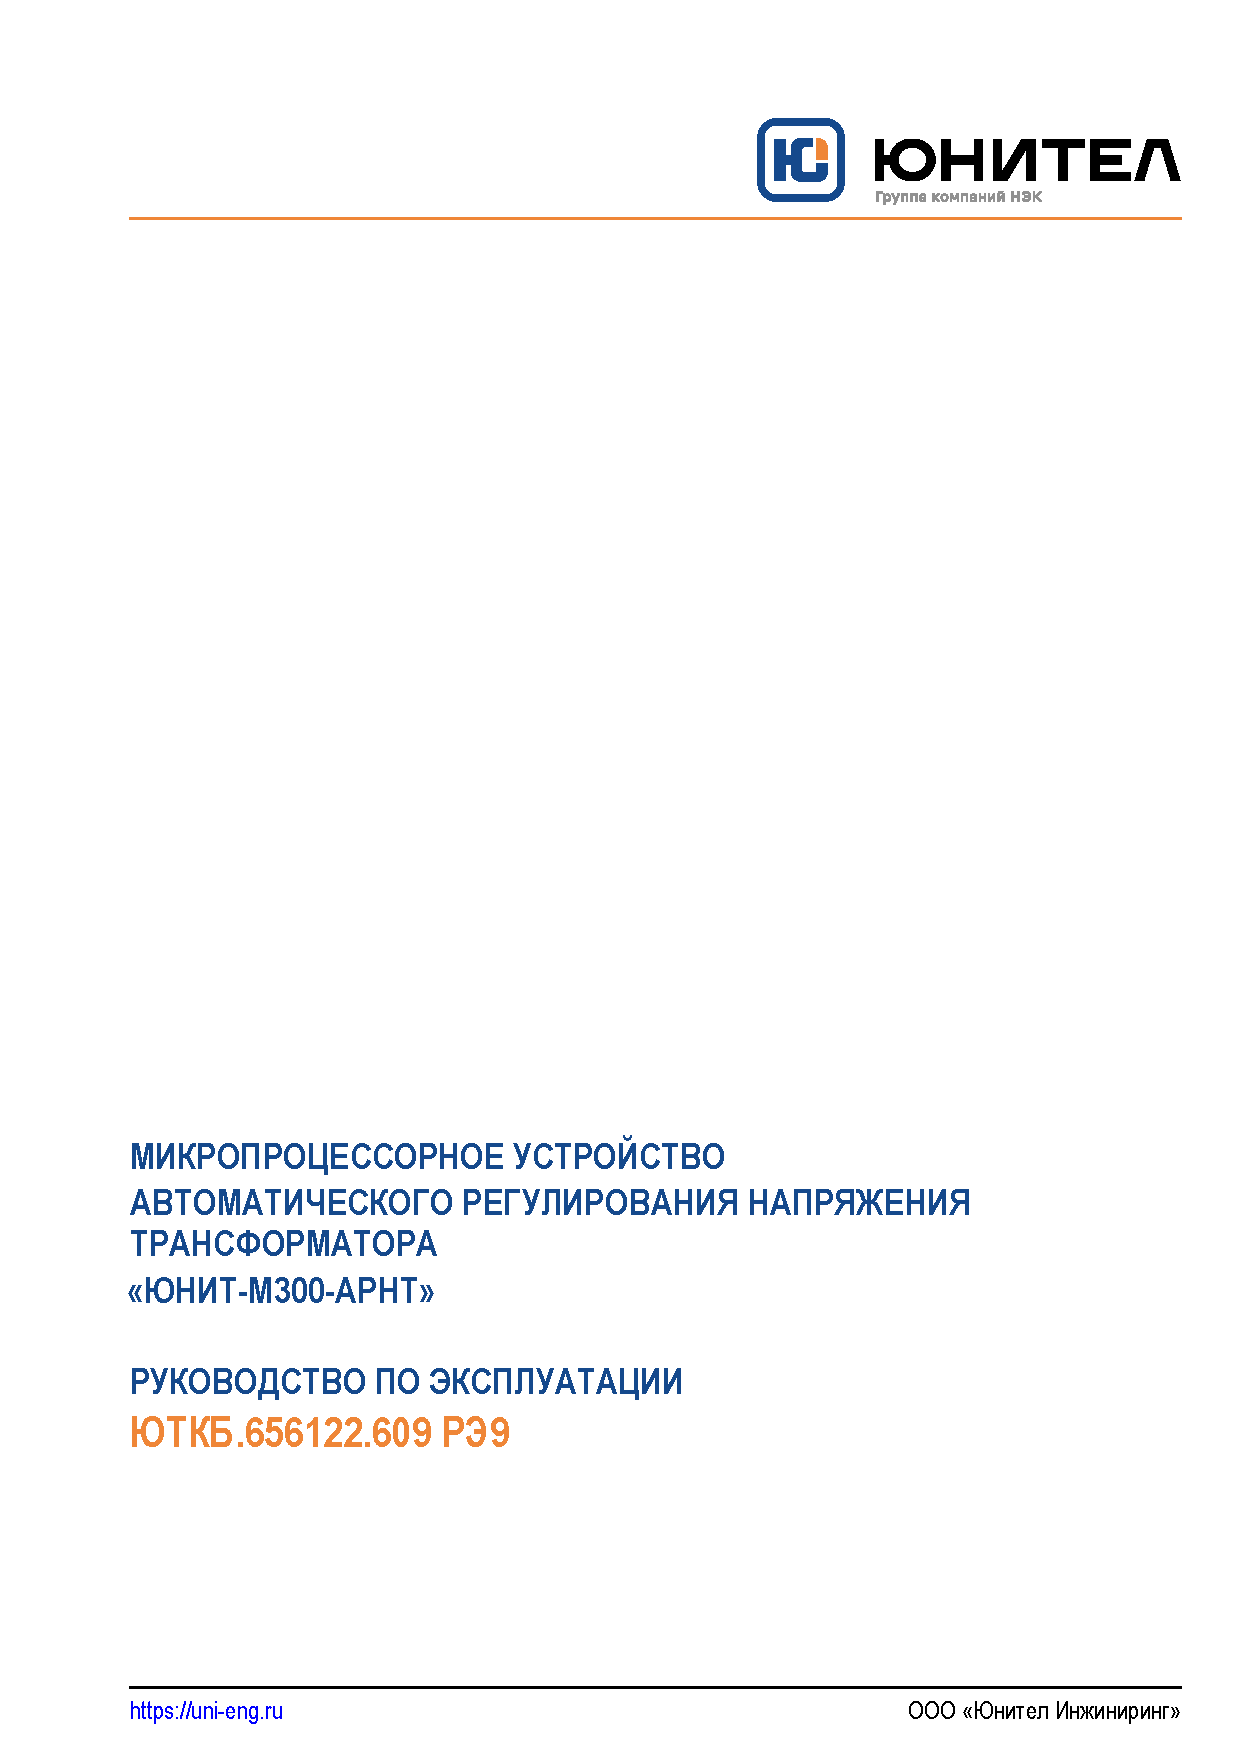
\includepdf[pages={1},width=0.5\textwidth, angle=90]{1.pdf} вставляем и поворачиваем pdf
%\begin{center}
%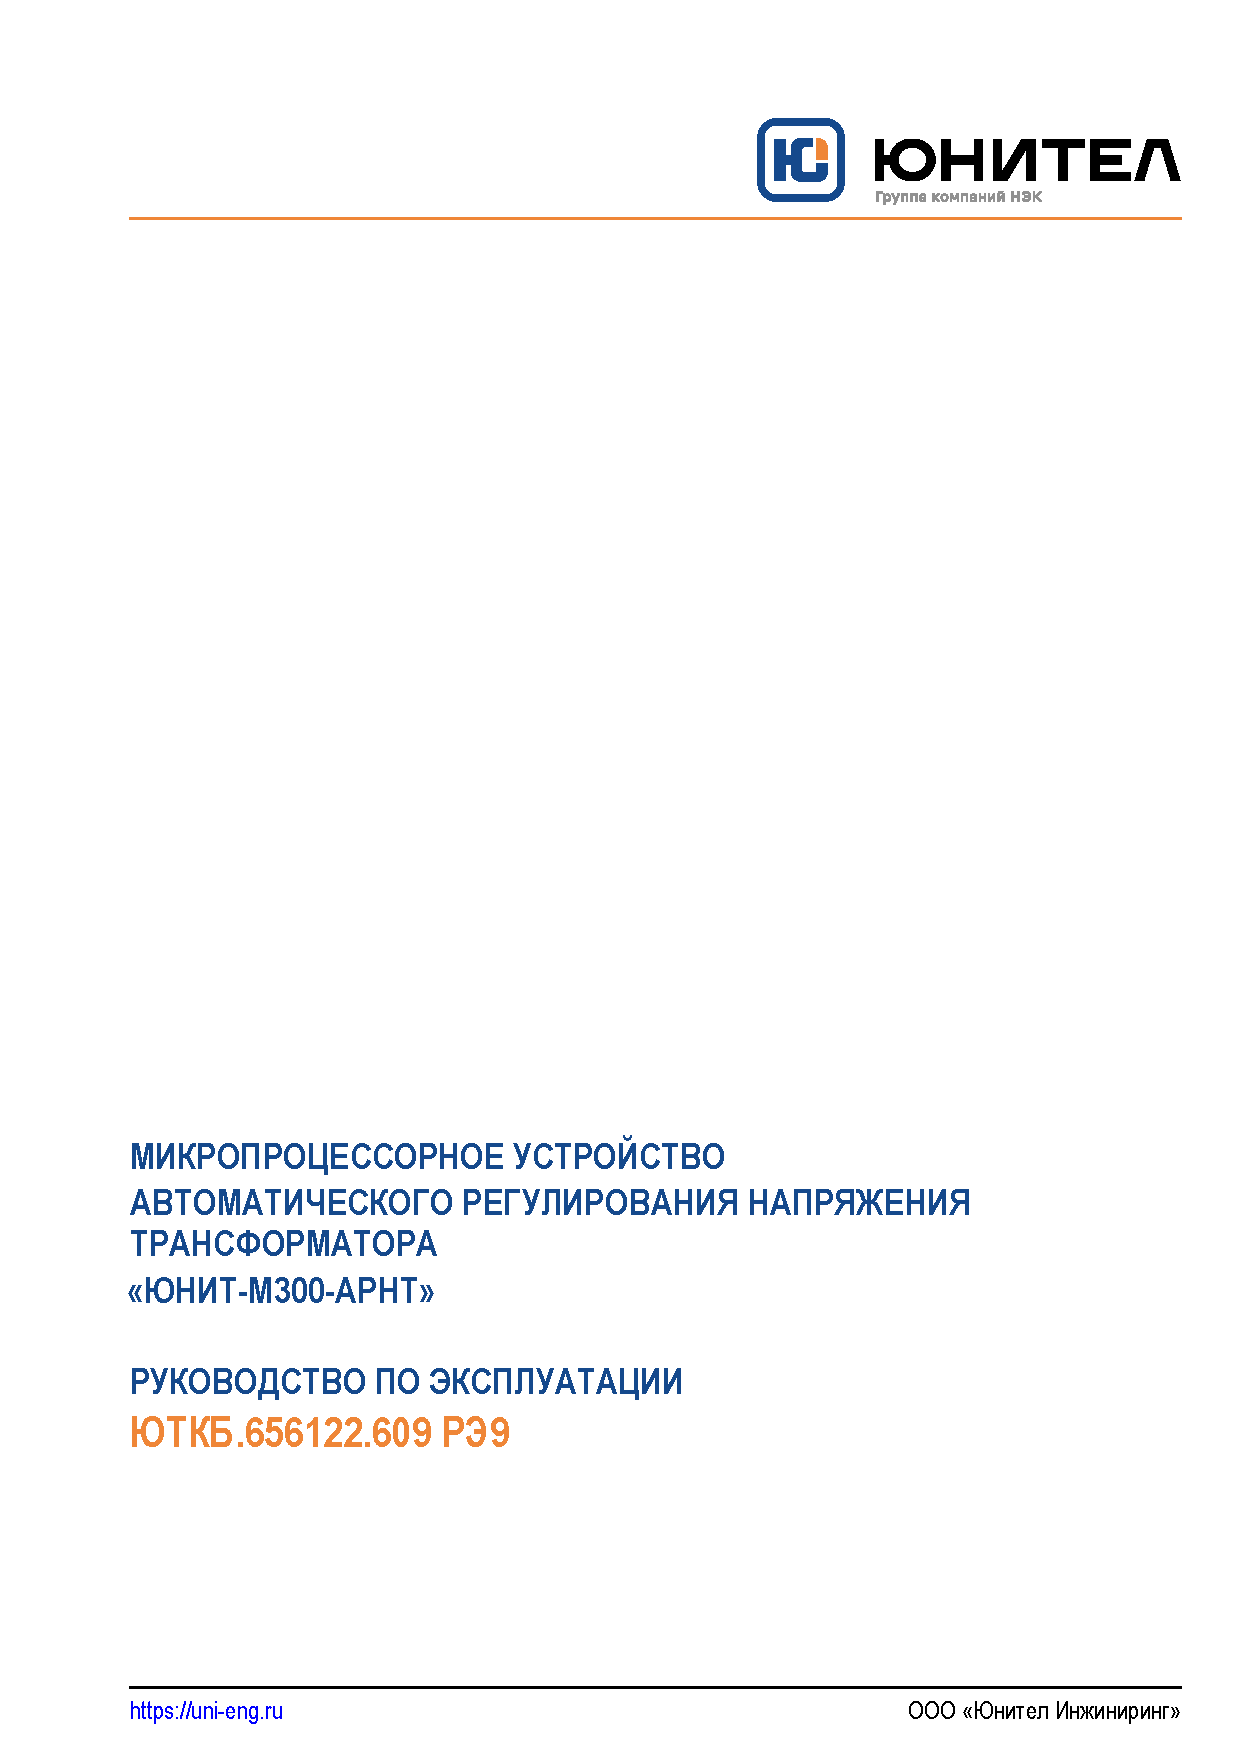
\includegraphics[width=1.4\textwidth]{1.pdf}
%\end{center}

\end{landscape}
\restoregeometry
